\documentclass[11pt,letterpaper]{article}
% arXiv-compatible preamble (pdflatex); Tectonic (XeTeX) compiles the same source.
\usepackage[utf8]{inputenc}
\usepackage[T1]{fontenc}
\usepackage{lmodern}
\usepackage[margin=1in]{geometry}
\usepackage{amsmath,amssymb}
\usepackage{graphicx}
\usepackage{booktabs,longtable,array,calc}
\usepackage{float}
\usepackage{pdflscape}
\usepackage{caption}
\captionsetup{labelformat=empty,font=small,skip=4pt}
\usepackage[numbers,sort&compress]{natbib}
\usepackage{xcolor}
\usepackage[hidelinks,breaklinks]{hyperref}
\usepackage{url}
\urlstyle{same}
\providecommand{\tightlist}{\setlength{\itemsep}{0pt}\setlength{\parskip}{0pt}}
\setlength{\parskip}{4pt plus 1pt}
\setlength{\emergencystretch}{2em}
\setlength{\parindent}{0pt}
\setlength{\LTpre}{6pt}\setlength{\LTpost}{6pt}
\setlength{\tabcolsep}{3pt}
\renewcommand{\arraystretch}{1.1}
\renewcommand{\topfraction}{0.95}\renewcommand{\bottomfraction}{0.9}\renewcommand{\textfraction}{0.05}\renewcommand{\floatpagefraction}{0.75}
\makeatletter\setlength{\@fptop}{0pt}\makeatother
\makeatletter\renewcommand{\@makefntext}[1]{\noindent\makebox[1.2em][l]{\@thefnmark}#1}\makeatother

\title{A Security Analysis of an Activation-Steering LLM Watermark: Key Recovery, Forgery, Scrubbing and Keyed Defences}
\author{Yichen Zhao\\ Independent Researcher\\ \texttt{alexyczhao@gmail.com}}
\date{Draft v0.1, assembled 2026-10-06}

\begin{document}
\maketitle

\begin{abstract}
Activation-steering watermarks add a secret vector to a hidden layer during generation and detect it from the model's internal activations when the text is re-read; their authors motivate the design by robustness to paraphrase. We present, to our knowledge, the first security analysis of such a watermark: the construction of LLM Self-Recognition \citep{ardoin2026selfrecognition}, re-implemented on Qwen2.5-1.5B at 256 tokens and measured under 6 pre-registered protocols against a passive attacker who holds the open weights and up to 1,024 watermarked outputs but cannot query the detector. First, under our measures the published strength did not reproduce on 1--3B base models: no strength made the scheme's trained probe reliably detectable without a perplexity cost. Second, that probe, re-trained by us, accepts steering that is not the key, so an attacker without the key produces fluent forgeries it accepts at the one strength where quality is acceptable (19.5\% against a bar of 14.3\%). Third, an exact key-resampling score test, a transfer of GaussMark's statistic to an additive activation vector, attributes 96.0--100.0\% of genuine texts at an exact 1\% false-positive rate (exact on average over keys; every key's rate checked) and rejects those forgeries. Fourth, the same statistic, averaged over 64 observed outputs, recovers the fixed key at the known layer (median cosine 0.940 and 0.951) and finds the layer for most keys when it searches, and its forgeries are attributed as often as genuine text (88.0 and 85.5\% against 86.5 and 90.0\% at the known layer; 86.0 and 87.5\% with the layer search from 256 texts); an activation-mean estimator recovers nothing from 1,024. Fifth, an off-the-shelf paraphrase scrubs the test's evidence at the quality-acceptable strengths (64.0 and 53.0\% success) and not above them. Sixth, keying the direction by the previous \(h\) tokens or rotating among 8 keys, transfers of context hashing and key rotation from token-level watermarking that the scheme's authors name as future work, blocks this attacker at \(n \leq\) 1,024: the context-keyed arms also improve perplexity but lose most of the paraphrase robustness, and rotation, whose quality is unchanged, falls to a clustering attacker from 64 texts at \(\rho = 0.50\) (and, post hoc, at 0.35). For the fixed key on this model, the strengths that are detectable and paraphrase-robust carry a quality cost (perplexity ratios 1.62 and 2.29), the quality-neutral strengths are scrubbed, and the published detector type is forgeable without the key at the quality-neutral strength (and, by plain acceptance, above it). The protocols, locks and code accompany the paper.
\end{abstract}

\hypertarget{introduction}{%
\section{Introduction}\label{introduction}}

Activation-steering watermarks mark text from inside the model: during generation a secret vector is added to one hidden layer at every token, and at detection the finished text is re-encoded with the same model and the signal is read from its activations rather than from token statistics. Their authors motivate the design by robustness to rewriting: for LLM Self-Recognition \citep{ardoin2026selfrecognition}, the scheme analysed here, ``Our method shows greater robustness to paraphrasing'' (p.~5), and detection is white-box by construction (``we assume white-box access to the internal activations of \(M\)'', p.~2).

Whether such a watermark is secure has not been measured. Its authors state the risk and leave it open: ``if an attacker can recover the secret steering vector and target layer, the watermark could be trivially reproduce to spoof the identity of the steered LLM'', and they propose as future work a vector that ``rotates or evolves during generation according to a pseudo-random schedule'' (p.~7). Stealing, forgery and scrubbing of token-level watermarks have an established literature \citep{jovanovic2024stealing, pang2024nofreelunch, gu2024learnability, zhang2026beyondseal}, and a September 2026 evaluation of it excludes model-internal schemes by scope \citep[p.~2]{li2026marksec}. To our knowledge, no prior work measures key recovery, forgery or scrubbing for an activation-steering watermark; search absence is not proof of novelty.

Regulators now name the properties measured here: the European Commission's Code of Practice on marking and labelling of AI-generated content (final, 10 June 2026) \citep{ec2026codeofpractice} expects an imperceptible watermark on free-form text longer than 200 tokens (Sub-measure 1.1.2, p.~9), measures \emph{reliability} by ``the error rate of the detection'' (Measure 3.2, p.~17) and asks that solutions ``maintain intended performance levels under varying conditions, covering both common alterations and adversarial attacks'', paraphrasing among them (Measure 3.3, pp.~17--18), and NIST AI 100-4 \citep{nist2024ai1004} defines a \emph{secure} watermark as one that resists attempts ``to remove or tamper with the watermark information, or to insert forged watermarks'' (p.~13). A false-positive rate (FPR) at a fixed level, detection after paraphrase and resistance to forged watermarks are the three measurements below (the quoted measures are in Appendix I); we use these texts for vocabulary and motivation only, and nothing here is a statement about any provider's compliance or deployment.

\textbf{What we do.} We re-implement Self-Recognition's construction on Qwen2.5-1.5B at 256 tokens (Section 2, Section 4) and measure it against a passive attacker who holds the open weights and up to \(n = \text{1,024}\) watermarked outputs, text only, and cannot query the detector (Section 2.2), under 6 pre-registered protocols locked by hash before any outcome existed (Section 4, App. A). Because the published strength does not transfer across models, strength is calibrated first as \(\rho\), the vector's norm relative to the activation norm, along the detectability--quality curve (Section 5.1). Five questions follow, one per results subsection: forgery of the published probe without the key (Section 5.2), the exact key test (Section 3, Section 5.3), key recovery from outputs (Section 5.4), scrubbing at matched quality (Section 5.5) and keyed directions with their price (Section 5.6).

\textbf{Contributions.} Every claim is bounded to one model (Qwen2.5-1.5B base), one layer, 8 keys, 256-token continuations, the strengths tested and this attacker family with \(n \leq \text{1,024}\); rates are medians over keys with cluster-bootstrap intervals and per-key tables (App. D).

\begin{enumerate}
\def\labelenumi{\arabic{enumi}.}
\tightlist
\item
  To our knowledge, the first security analysis of an activation-steering LLM watermark (key recovery, forgery, scrubbing, an exact test and a keyed defence), on one published scheme, re-implemented; SLAM and AWM are discussed, not tested.
\item
  The scheme's published detector type, a trained per-token probe re-implemented and re-trained by us, accepts steering that is not the key (median cosine at most 0.062 with it) and degenerate text; fluent, non-repetitive forgery without the key is practical at \(\rho = 0.35\) (fluent acceptance 19.5\% against a bar of 14.3\%) and inconclusive at 0.50 and 0.70. The authors note that paraphrased human text spoofs their detector (p.~5), and under our conditions their published setting did not reproduce on 1--3B base models (Section 5.1, with their numbers beside ours).
\item
  An exact key-resampling score test, a transfer of GaussMark's statistic \citep{block2025gaussmark} to an additive activation vector, attributes 96.0--100.0\% of genuine texts at an exact 1\% false-positive rate (exact on average over keys; every study key calibrated), beats the probe at \(\rho \leq 0.50\), attributes random-key text at a median rate of 0.0\% (single keys up to 4\%), and makes those forgeries not practical for the median key.
\item
  The first measured key-recovery attack on such a watermark (search level): the test's own statistic, averaged over 64 outputs, recovers the fixed key at the known layer (median cosine 0.940 and 0.951 at \(\rho = 0.35\) and 0.50; the layer search finds it for 6 and 6 of 8 keys), and its forgeries are attributed as often as genuine text (88.0 and 85.5\% against 86.5 and 90.0\% at the known layer; 86.0 and 87.5\% with the layer search from 256 texts), where the activation-mean estimator recovers nothing from 1,024 (cosine at most 0.16). That the detector's best statistic is the thief's best estimator is a measured fact with an inferential explanation (Section 3); the token-level budget comparison carries an access caveat (Section 5.4).
\item
  To our knowledge the first scrubbing evaluation of such a watermark under an exact, per-key-calibrated test at matched quality (the authors' own paraphrase figures are robustness measurements, not attack evaluations; Section 6), with an insider (true-key) bound: an off-the-shelf paraphrase succeeds 64.0 and 53.0\% of the time at \(\rho = 0.25\) and 0.35 and is not effective at 0.50 and 0.70; the comparison with the authors' robustness figures is indirect.
\item
  The measured trade-off along \(\rho\) for the fixed key on this model (an interpretation, labelled): the detectable and paraphrase-robust strengths cost perplexity (ratios 1.62 and 2.29), the quality-neutral strengths are scrubbed, and the probe is forgeable at the one strength where quality is acceptable; we are not the first to note a trade-off (Section 6).
\item
  Context keying (\(h = 1, 4\)) and rotation among 8 keys, transfers of context hashing \citep{kirchenbauer2023watermark, kirchenbauer2024reliability} and key rotation \citep{kirchenbauer2023watermark, pang2024nofreelunch, gu2024learnability, dathathri2024synthid} to activation steering, named as future work by Ardoin et al.~(p.~7): both hashed arms block this attacker at \(n \leq \text{1,024}\) (forgeries attributed at most 9.0\%) and improve perplexity, but lose most of the paraphrase robustness (material for \(h = 1\) at both strengths and \(h = 4\) at 0.50, inconclusive for \(h = 4\) at 0.35); rotation keeps robustness and falls to a clustering attacker from 64 texts at \(\rho = 0.50\) (95\% attributed), and at 0.35 only through a labelled post-hoc addendum beside the pre-registered ``blocked'' verdict (Section 5.6).
\end{enumerate}

Two practical points are restated for this family, as others have noted: a deployer with one key should check its own false-positive rate on paraphrased null text, since resampling p-values are exact only on average over keys (Section 5.5), and a quality bar for forgery or scrubbing must pair perplexity with a repetition term and be read against reference samples (Section 2.2). Per-key heterogeneity, the probe's acceptance of paraphrases at high strength and the reading that the probe detects steering rather than the key are a descriptive, a lead and an inference, labelled where they appear. We do not claim the first stealing attack on LLM watermarks, a new watermark, immunity to stealing, a fix of the trade-off, or results beyond the model, budgets and attackers tested (Section 7). The protocols, locks and code accompany the paper (Section 8).

\hypertarget{background-and-threat-model}{%
\section{Background and threat model}\label{background-and-threat-model}}

\hypertarget{the-scheme}{%
\subsection{The scheme}\label{the-scheme}}

An activation-steering watermark adds a secret vector to the model's hidden state during generation and detects it by re-encoding the finished text with the same model and reading the hidden state back. We analyse the construction of Self-Recognition \citep{ardoin2026selfrecognition}. Given a direction \(v \in \mathbb{R}^d\) and a coefficient \(\alpha > 0\), its authors ``add the scaled vector to the intermediate activation at layer \(l\) at each token generation step'' (p.~2), \(A_l(x_i) \leftarrow A_l(x_i) + \alpha v\). The direction is random and sparse, ``sampled from \(U([-1, 1]^d)\), with 99.7\% of dimensions set to zero'' (p.~11), so a key on a model of width \(d = 1536\) has \(k = 4\) non-zero coordinates; the published strength is \(\alpha = 5\), and ``Injection and detection are performed at the middle layer'' (p.~11). Detection is white-box (``we assume white-box access to the internal activations of \(M\)'', p.~2): the text is re-encoded and a multilayer perceptron (MLP) probe on the layer-\(l\) activations decides, ``The MLP has two hidden layers of width 32, trained for a single epoch to predict the steering index \(k\) of a given extracted activation'' (p.~3), with token decisions aggregated to a text decision; a training-free alternative is the cosine similarity between the activations and the key (p.~6).

We re-implement the scheme on Qwen/Qwen2.5-1.5B (Section 4) and the detector as the authors' public code defines it: an MLP on raw per-token activations at the steered layer, trained for one epoch on the owner's own watermarked and unwatermarked texts and scored as the mean token probability of the watermarked class (App. A). An owner must fix a false-positive rate, so the score is thresholded at the 99th percentile of the owner's own unwatermarked texts (nominal 1\%), and we report acceptance at that threshold rather than the accuracies the authors report. Two definitions are ours. \textbf{Strength:} \(\alpha\) does not transfer across models, because activation norms differ by model and layer, so we measure \(\rho = \lVert v \rVert / N\), with \(N\) the median token activation norm at the steered layer over unsteered text (\(N = 56.90\) here); the published \(\alpha = 5\) maps to very different \(\rho\) on the models we tried (Section 5.1). \textbf{Working range:} at the strengths studied, \(\rho \in \{0.25, 0.35, 0.50, 0.70\}\), the probe does not detect the lower strengths reliably and the higher strengths cost perplexity (Section 5.1), so the attacks run along that curve rather than at one setting.

\hypertarget{threat-model}{%
\subsection{Threat model}\label{threat-model}}

We follow Kerckhoffs's principle \citep{kerckhoffs1883cryptographie}, as the nearest keyed activation scheme does \citep{aremu2026awm}: the weights, the scheme (including \(k\) and the candidate layers), \(\rho\) and the detector's form are public; the direction \(v\), the layer \(l\) and the owner's private detector data (the trained probe and its threshold; for the exact test of Section 3, nothing beyond \(v\) and \(l\)) are secret.

The \textbf{attacker} is passive. It holds the open weights and observes \(n\) watermarked continuations at one strength, text only, without their prompts (\(n \in \{64, 256, 1024\}\) for forgery, \(n \in \{1, 4, 16, 64, 256, 1024\}\) for recovery). It can generate unlimited unwatermarked text on its own prompts and re-encode any text through the open model, so it sees activations and gradients at every layer. It cannot query the owner's detector and never sees \(v\), the probe, its threshold, the owner's reference texts or the evaluation prompts; the layer \(l\) is withheld too, except in two readings that say so, the fixed key's known-layer estimate (Section 5.4) and the keyed arms (Section 5.6); the attack code receives features and public parameters only, which every protocol's validation asserts (App. A). The \textbf{owner} knows \(v\) and \(l\), calibrates its detector on its own unwatermarked texts and sees only the text at detection time.

Three goals are measured, in the terms of the token-level security literature \citep[p.~3]{li2026marksec}: stealing ``aims to recover reusable watermark-related information''; ``Scrubbing aims to transform a watermarked text \(y_w\) into an attacked text \(y_a\) that is no longer detected as watermarked while preserving text quality''; ``Spoofing aims to generate a forged text \(y_s\) that is accepted as watermarked without being produced by the genuine watermarking process''.

\begin{itemize}
\tightlist
\item
  \textbf{Recovery:} \(\cos(\hat v, v)\) between the estimate and the key, whether the estimated layer equals \(l\), and the share of the support recovered.
\item
  \textbf{Forgery} (spoofing): new text, generated by the attacker on prompts it does not control, counts only if the owner's detector \textbf{accepts} it at the 1\% threshold \textbf{and} it is as fluent and as non-repetitive as the owner's genuine watermarked texts (perplexity and seq-rep-4 \citep{welleck2020unlikelihood} at most the genuine 95th percentiles; Section 4); the share meeting all three conditions is the \textbf{fluent acceptance} (FA). Forgery is \textbf{practical} at a strength if, at some \(n\), the median FA over keys reaches half the genuine FA and its lower confidence bound exceeds the upper bound of a \textbf{random-key control} (a fresh key of the same distribution and norm: what generic steering alone achieves). This is the quality-constrained success of the token-level evaluations \citep{li2026marksec}, with proxies in place of a judge.
\item
  \textbf{Scrubbing:} a watermarked text is transformed; the transformation \textbf{succeeds} if the detector no longer detects it \textbf{and} four quality conditions hold (fluency, repetition, length, meaning; Section 4), against the detector's miss rate on the untouched originals or random edits of the same size.
\end{itemize}

The budgets differ in kind from the token-level literature, whose attackers query a black-box API with ``\(n = 30{,}000\) responses of token length \(\leq 800\)'' \citep[p.~6]{jovanovic2024stealing}, ``2.2 million tokens in total'' \citep[p.~6]{pang2024nofreelunch} or ``2,000 victim watermarked texts'' \citep[p.~8]{zhang2026beyondseal} and ``has only blackbox access to full generations'' \citep[p.~3]{jovanovic2024stealing}; ours has at most 1,024 texts of 256 tokens but re-encodes them through the model that produced them. A perplexity bar alone admits degenerate text, since ``a highly repetitive, degenerate loop often yields low PPL'' \citep[p.~14]{ardoin2026selfrecognition}, and SLAM scores quality on four axes \citep{harelcanada2026slam}; our first fluency rule was perplexity only and most of its accepted forgeries at the strongest setting were loops (an exploratory reading, labelled; Section 5.2, App. E), so every later rule pairs perplexity with seq-rep-4 on both sides, the attacker's self-check and the evaluation, and fixed samples of passing texts are read (App. H). Both points have been made before; we restate them for this family.

\hypertarget{attack-routes}{%
\subsection{Attack routes}\label{attack-routes}}

Three routes are compared against the attacker's own unwatermarked reference texts (pool C, 2,000 texts; Section 4), coordinate by coordinate and layer by layer, as \(z\)-scores of the mean difference of a per-text feature (App. C).

\textbf{Route A} (key recovery from activations) takes the layer with the largest \(|z|\) of the token-mean activation, the \(k\) coordinates with the largest \(|z|\) there as the support and the mean differences as values, rescaled to \(\rho\) times the attacker's own median norm.

\textbf{Route B} (footprint imitation) estimates no key and copies the dense mean difference at the layer with the largest \(z\)-norm, rescaled.

\textbf{Route A\ensuremath{'}} (key recovery from the detector's statistic) applies Route A's rule to the standardised gradient of the continuation log-likelihood with respect to an additive vector at each layer, the exact test's own statistic (Section 3), averaged over the observed texts, per observable context against context-keyed directions and per cluster (or on the whole mixture) against rotation.

From Study 1 v0.3 the attacker screens five candidate layers with 16 trial generations each, keeping those no less fluent than the observed texts (and, from v0.4, no more repetitive), since it cannot query the detector.

The \textbf{scrubbing attackers} are two off-the-shelf paraphrasers (P-Qwen, P-Phi; Section 4) with an attacker-side quality self-check and up to three attempts, and key-guided word substitutions at 2, 5 and 10\% of the tokens steered by the true key (E-true, an insider bound), by the Route A estimate (E-est) or at random (E-rand).

Forgeries are 100 continuations per condition on fixed evaluation prompts (pool D), scored by the owner's detector beside the \textbf{oracle} (the true key at the true layer) and \textbf{random-key} controls on the same prompts. A rule asks at every strength whether the random key alone reaches half the oracle's rate (``generic steering suffices''), in which case forgery would need no key.

\hypertarget{an-exact-key-test-for-additive-activation-vectors}{%
\section{An exact key test for additive activation vectors}\label{an-exact-key-test-for-additive-activation-vectors}}

The probe of Section 2.1 detects a learned footprint, on our reading of Section 5.2. A detector of the \emph{key} needs no training, as a transfer of GaussMark's score test \citep{block2025gaussmark}. GaussMark watermarks by perturbing weights, ``Sample watermark key \(\xi \sim N(0, \sigma^2 I)\)'' and ``Watermark model by setting \(\theta(\xi) = \theta + \xi\)'' (Alg. 1, p.~6), ``in only a single feedforward layer'' (p.~5), and detects with \(\psi(y, \xi \mid x) = \langle \xi, \nabla_\theta \log p_\theta(y \mid x) \rangle / (\sigma \lVert \nabla_\theta \log p_\theta(y \mid x) \rVert)\), rejecting when \(\psi \geq \Phi^{-1}(1 - \alpha)\) (Alg. 2, p.~7), because ``the distribution of \(\psi(y, \xi \mid x)\) \ldots{} is always a standard normal under \(H_0\) because \(y\) is independent of \(\xi\)'' (p.~9). This is the score statistic for the perturbation \citep{rao1948score}: to first order, text generated under the perturbed model shifts the expected gradient along the perturbation. In an activation-steering watermark the perturbation is an additive vector \(b\) at the output of layer \(l\), so the statistic is the gradient of the text's log-likelihood with respect to \(b\) at \(b = 0\), projected on the key. Two things change the calibration: the keys are sparse with uniform values, not Gaussian, so the null law cannot be read from \(\Phi\); and the gradient's coordinates have very different scales, so a raw projection depends on a few outlier dimensions. We therefore standardise and resample keys.

\textbf{The statistic S4 and its exact p-value.} One forward and one backward pass over a text's first 256 continuation tokens (no prompt) gives \(g = \partial \log p(y) / \partial b \,|_{b = 0} \in \mathbb{R}^{1536}\) at layer 14. The owner centres and scales each coordinate against its own unwatermarked reference texts (pool F, 200 texts), \(x = (g - \mu_F) / \sigma_F\), and computes \(T(x, v) = \langle x, v \rangle / (\lVert x \rVert \lVert v \rVert)\). With \(M = 999\) null keys \(v_1, \dots, v_M\) drawn from the scheme's public key distribution (fixed seeds, disjoint from every other key), \(p = (1 + \#\{j : T(x, v_j) \geq T(x, v)\}) / (1 + M)\) \citep{phipson2010permutation}, and a text is attributed to \(v\) when \(p \leq 0.01\). The true-positive rate (TPR) is the share of genuine watermarked texts attributed to their key. If the text was produced independently of \(v\) (unwatermarked, human, or steered by another key), \(v\) and the null keys are exchangeable, so \(P(p \leq \alpha) \leq \alpha\) \textbf{exactly, on average over the draw of the key}. GaussMark's authors state the same limit of their guarantee: the bounds ``are valid for any fixed \(x \in \mathcal{X}\), but are marginalized over the key \(\xi\)'' (p.~11). A deployer holds one key, whose own false-positive rate need not equal \(\alpha\); we never claim exactness for every key. The protocols therefore add a \textbf{per-key calibration gate}: a key is calibrated if its false-positive rate on 1,000 of the owner's unwatermarked texts is at most 3\%, and the pooled rate must lie in {[}0.3, 2.5{]}\%. On the study keys the pooled rate was 0.81\%, 8 of 8 keys were calibrated (0.1--1.7\%), and the pooled rate on human continuations was 0.68\% (Table A3).

\textbf{Why standardise.} A pilot on four tuning keys compared, under the same resampling test, the raw cosine of the token-averaged activations (S1, the scheme's training-free statistic), its standardised form (S2), the raw gradient score (S3) and the standardised gradient score (S4): the gradient statistics detected 96--98\% (S3) and 94--98\% (S4) of single texts at an exact 1\% false-positive rate at the working strengths, the raw cosine 0\% (Table A2). It also exposed the per-key issue: because the raw activation mean is nearly the same vector for every text, a key's rank among the null keys is almost fixed, and over 1,000 random keys S1 fired on more than half of the null texts for 1.1\% of keys while its mean rate stayed 1.15\% (an exploratory diagnosis, App. B); standardisation kept every key at most 4.75\% (S4). S4 was chosen as the primary statistic by decision after that diagnosis; the pilot's pre-set selection rule is reported as written in App. B.

\textbf{Two variants used by the defence (Section 5.6).} For \textbf{rotation} among \(K\) keys the owner tests the union, \(U = \max_k \langle x, v_k \rangle\), with the null from 999 disjoint groups of \(K\) public null keys, so the level is exact by the same argument: a transfer of the multi-key design of Kirchenbauer et al. \citep{kirchenbauer2023watermark}, ``we run \(k\) tests, one for each of the possible keys'' (p.~7), with a resampled maximum in place of a Bonferroni correction. For a \textbf{context-keyed} direction \(v(c_t)\), derived by a keyed pseudorandom function from the secret and the previous \(h\) tokens, the owner takes the per-position gradients \(g_t\) (one backward pass), standardises them with pooled position statistics from pool F and sums the projections on each position's own key, \(S(x, m) = \sum_t \langle x_t, v_m(c_t) \rangle\), with the p-value from 999 resampled secrets; the contexts are read from the text itself (App. B).

\textbf{Why the same statistic is the thief's estimator} (an inference; the measurement is Section 5.4). To first order the expected gradient of a text steered by \(v\) is \(\mathbb{E}[g] \approx F v\), with \(F\) the Fisher information of \(b\) at 0, which is what gives \(\langle g, v \rangle\) its power; the same relation says that the \textbf{mean} of \(g\) over many observed outputs estimates \(F v\), and after the per-coordinate standardisation the attacker performs against its own reference texts, a sparse estimate of that mean points along \(v\). Route A\ensuremath{'} (Section 2.3) is this estimator; it needs the open weights and the observed texts, not the detector. App. B sketches the first-order argument and its assumptions; we present it as the reason we expected the recovery, not as a proof. On the tuning keys the estimator reached a median cosine of 0.80 from 4 texts and 0.95 from 16 at \(\rho = 0.35\), 0.93 from 64 at \(\rho = 0.50\) and 0.57 from 100 at \(\rho = 0.70\), where Route A's activation mean reached at most 0.087 (Table A5); the study keys follow in Section 5.4.

\hypertarget{experimental-setup}{%
\section{Experimental setup}\label{experimental-setup}}

\textbf{Model and keys.} The target is Qwen/Qwen2.5-1.5B (base, revision \texttt{8fae\allowbreak{}d761}, apache-2.0) \citep{qwen2024qwen25, qwen2024card15b} in bfloat16 on Apple silicon; \(d = 1536\), 28 decoder layers; steering and detection at the output of layer 14, the middle layer. Keys follow the scheme's construction, \(k = 4\) non-zero coordinates (\(\lfloor 0.003 \cdot d \rfloor\)) with values uniform in \([-1, 1]\), rescaled to norm \(\rho N\), \(N = 56.90\). The \textbf{study keys} are the seeds 1001--1008 (8 keys), first used in Study 1 v0.2 and reused unchanged by every later study; the \textbf{random-control keys} are 5001--5008; four \textbf{tuning keys} (9001--9004) served the calibrations and pilots and appear in no study result. Strengths are \(\rho \in \{0.25, 0.35, 0.50, 0.70\}\) (Study 5: 0.35 and 0.50). Generation uses the scheme's sampling (temperature 0.7, top-p 0.9, top-k 50, repetition penalty 1.1) and exactly 256 new tokens; every detector and attacker feature is computed from the continuation only.

\textbf{Prompts and pools.} Prompts are the first 40 words of documents from the C4 realnewslike validation shard \citep{raffel2020t5} (13,863 records, 0 parse failures, 8,580 documents of at least 240 words), with the next 200 words kept as the \textbf{human continuation}. A fifth of the units, by ID hash, is a \textbf{holdout} (1,684 units) sealed in the loader, which refuses to serve it without a final protocol lock; it was never used. The 6,896 development units are assigned once, by hash rank, to disjoint pools A--F, whose sizes and roles are in Table 1's note: the owner's unwatermarked null texts with their human continuations (A), the attacker's observed and reference prompts (B, C), the evaluation prompts for forgeries and controls (D) and the owner's probe-training texts (E, F). The owner's training texts are disjoint from its threshold, check and evaluation texts, and the attacker's prompts from all of them. WikiText-103 \citep{merity2017pointer} was frozen as a second domain and is not used by the results reported.

\textbf{Detectors.} The probe is trained per key and strength on the layer-14 token activations of pool E against pool F, scored as the mean token probability and thresholded at the 99th percentile of pool A1 (nominal 1\% false-positive rate, checked on A2). The exact test S4 (Section 3) uses \(M = 999\) null keys at \(p \leq 0.01\), with a stricter secondary reading at 9,999 null keys and \(p \leq 0.001\). Both see the continuation only.

\textbf{Paraphrasers, editors and quality proxies.} P-Qwen is Qwen2.5-1.5B-Instruct \citep{qwen2024card15binstruct} and P-Phi is Phi-3.5-mini-instruct \citep{abdin2024phi3}, each given the continuation with the fixed paraphrase instruction \texttt{PROMPTS{[}"P2"{]}} from \texttt{research/\allowbreak{}study2\_\allowbreak{}pilot/\allowbreak{}scrub\_\allowbreak{}core.\allowbreak{}py}, selected by \texttt{research/\allowbreak{}study2/\allowbreak{}common\_\allowbreak{}s2.\allowbreak{}py}, in its chat template (App. C), sampled at temperature 0.7 and top-p 0.9 with at most 400 new tokens; the attacker keeps the first of up to three attempts that passes its own quality check. The editor replaces whole words by likely alternatives at the positions a first-order estimate marks as contributing most to the detector's statistic, in rounds of 5\% of the tokens, saved at 2, 5 and 10\% (App. C). Quality is measured by proxies, not by human judgement: perplexity under the unsteered model given the prompt; seq-rep-4 \citep{welleck2020unlikelihood}; token length; and the cosine between all-mpnet-base-v2 sentence embeddings \citep{reimers2019sbert} of a scrubbed text and its original. A forgery is fluent if its perplexity and seq-rep-4 are at most the 95th percentiles of the owner's genuine watermarked texts at that key and strength. A scrub passes if its perplexity stays within \(\max(1.25 \times\) the original's, the 95th percentile of pool A's human continuations\()\) and its seq-rep-4 within \(\max(\)the original's, that 95th percentile\()\) (perplexity 25.4, seq-rep-4 0.048), its length is at least 80\% of the original's and its embedding cosine exceeds 0.825, the 95th percentile over pool A's same-prompt pairs of a model continuation and the human continuation; the attacker's self-checks use the same forms on its own pool C data (perplexity 22.2, seq-rep-4 0.048, cosine 0.810). Stricter readings (the model-text 95th percentile, perplexity 7.3; the human median, 12.9) are secondaries, and fixed samples of forged, scrubbed and genuine texts are read (App. H).

\textbf{Uncertainty.} The key is the unit of independence; texts are nested in keys. Every rate is the median over the 8 keys of the per-key rate, with a 95\% interval from a cluster bootstrap over keys and then texts (\(B\) = 2,000) \citep{davison1997bootstrap}; contrasts between two detectors or two methods on the same texts use paired resampling. Beside every median we report the number of keys meeting the bar, with per-key tables in App. D, because a median can pass while a few keys fail completely; counts of keys carry Clopper--Pearson intervals \citep{clopper1934binomial}.

\textbf{Pre-registration and compute.} Each study has a protocol fixing its question, information timing, metrics, materiality thresholds, rules and stop rules, and code validated on inputs only (synthetic data and the tuning keys) before any outcome exists; the protocol, the code and every reused input file are hashed into a lock file, and the runners verify every hash before and after each phase and refuse otherwise. A correction becomes a new version with the earlier verdicts standing (Study 1 v0.2 \ensuremath{\rightarrow} v0.3 \ensuremath{\rightarrow} v0.4); every rule's bounds were checked at the extremes before locking; readings added after a run are labelled exploratory or post hoc wherever they appear. \textbf{Table 1} lists the 6 locked studies with their rules, bars, design, lock dates and run times; App. A gives every pilot and specification (Table A1). Everything ran on one Apple-silicon laptop (M5, 16 GB unified memory) with PyTorch 2.14.0; the six runs took 91.1 h in total (22.4, 6.4, 6.5, 2.9, 26.6 and 26.3 h), with model weights, prompt corpora and paraphrasers pinned by revision and file hash.

{\scriptsize\setlength{\tabcolsep}{1.5pt}\begin{longtable}[]{@{}
  >{\raggedright\arraybackslash}p{(\columnwidth - 18\tabcolsep) * \real{0.0459}}
  >{\raggedright\arraybackslash}p{(\columnwidth - 18\tabcolsep) * \real{0.1378}}
  >{\raggedright\arraybackslash}p{(\columnwidth - 18\tabcolsep) * \real{0.1413}}
  >{\raggedright\arraybackslash}p{(\columnwidth - 18\tabcolsep) * \real{0.1413}}
  >{\raggedright\arraybackslash}p{(\columnwidth - 18\tabcolsep) * \real{0.0848}}
  >{\raggedright\arraybackslash}p{(\columnwidth - 18\tabcolsep) * \real{0.0742}}
  >{\raggedright\arraybackslash}p{(\columnwidth - 18\tabcolsep) * \real{0.1272}}
  >{\raggedright\arraybackslash}p{(\columnwidth - 18\tabcolsep) * \real{0.0919}}
  >{\raggedright\arraybackslash}p{(\columnwidth - 18\tabcolsep) * \real{0.0353}}
  >{\raggedright\arraybackslash}p{(\columnwidth - 18\tabcolsep) * \real{0.1201}}@{}}
\caption{\textbf{Table 1.} The six locked studies: question, pre-registered rules and bars, design, lock and run}\tabularnewline
\toprule\noalign{}
\begin{minipage}[b]{\linewidth}\raggedright
Study
\end{minipage} & \begin{minipage}[b]{\linewidth}\raggedright
Question
\end{minipage} & \begin{minipage}[b]{\linewidth}\raggedright
Pre-registered rules
\end{minipage} & \begin{minipage}[b]{\linewidth}\raggedright
Materiality bars
\end{minipage} & \begin{minipage}[b]{\linewidth}\raggedright
Keys; strengths \ensuremath{\rho}
\end{minipage} & \begin{minipage}[b]{\linewidth}\raggedright
Attacker budget n
\end{minipage} & \begin{minipage}[b]{\linewidth}\raggedright
Locked (UTC date); protocol SHA-256
\end{minipage} & \begin{minipage}[b]{\linewidth}\raggedright
Commit
\end{minipage} & \begin{minipage}[b]{\linewidth}\raggedright
Run (h)
\end{minipage} & \begin{minipage}[b]{\linewidth}\raggedright
Results
\end{minipage} \\
\midrule\noalign{}
\endfirsthead
\toprule\noalign{}
\begin{minipage}[b]{\linewidth}\raggedright
Study
\end{minipage} & \begin{minipage}[b]{\linewidth}\raggedright
Question
\end{minipage} & \begin{minipage}[b]{\linewidth}\raggedright
Pre-registered rules
\end{minipage} & \begin{minipage}[b]{\linewidth}\raggedright
Materiality bars
\end{minipage} & \begin{minipage}[b]{\linewidth}\raggedright
Keys; strengths \ensuremath{\rho}
\end{minipage} & \begin{minipage}[b]{\linewidth}\raggedright
Attacker budget n
\end{minipage} & \begin{minipage}[b]{\linewidth}\raggedright
Locked (UTC date); protocol SHA-256
\end{minipage} & \begin{minipage}[b]{\linewidth}\raggedright
Commit
\end{minipage} & \begin{minipage}[b]{\linewidth}\raggedright
Run (h)
\end{minipage} & \begin{minipage}[b]{\linewidth}\raggedright
Results
\end{minipage} \\
\midrule\noalign{}
\endhead
\bottomrule\noalign{}
\endlastfoot
Study 1 v0.2 & Key recovery and forgery against the trained probe, along \ensuremath{\rho} & G1 null calibration; G2 attack isolation; L1 working watermark; R1 recovery; R2 forgery practical; R3 generic steering suffices & R1: median cos \ensuremath{\geq} 0.9 and layer hit for \ensuremath{\geq} 7 of 8 keys; R2: acceptance \ensuremath{\geq} 50\% of the oracle's and the lower bound above the random-key control & 1001--1008; \ensuremath{\rho} \ensuremath{\in} \{0.25, 0.35, 0.50, 0.70\} & recovery \{1, 4, 16, 64, 256, 1,024\}; forgery \{64, 256, 1,024\} & 2026-09-26; \texttt{8794\allowbreak{}f4dd\allowbreak{}b25e} & \texttt{99d9\allowbreak{}7978} & 22.4 & \texttt{research/\allowbreak{}outputs/\allowbreak{}study1\_\allowbreak{}v0.\allowbreak{}2/\allowbreak{}results.\allowbreak{}json} \\
Study 1 v0.3 & Fluent forgery (perplexity condition) with the attacker's own layer search & integrity check; F1 fluent forgery practical; F3 fluent generic steering suffices & F1: fluent acceptance \ensuremath{\geq} 50\% of the oracle's and the lower bound above the random-key control & 1001--1008; \ensuremath{\rho} \ensuremath{\in} \{0.35, 0.50, 0.70\} & \{64, 256\} & 2026-09-27; \texttt{842b\allowbreak{}71fc\allowbreak{}4624} & \texttt{8b87\allowbreak{}18de} & 6.4 & \texttt{research/\allowbreak{}outputs/\allowbreak{}study1\_\allowbreak{}v0.\allowbreak{}3/\allowbreak{}results.\allowbreak{}json} \\
Study 1 v0.4 & Fluent, non-repetitive forgery (perplexity and seq-rep-4 conditions on both sides) & integrity check; F1; F3 & F1 as v0.3 with the repetition term & 1001--1008; \ensuremath{\rho} \ensuremath{\in} \{0.35, 0.50, 0.70\} & \{64, 256\} & 2026-09-28; \texttt{ab24\allowbreak{}0e34\allowbreak{}1a6c} & \texttt{6c62\allowbreak{}36be} & 6.5 & \texttt{research/\allowbreak{}outputs/\allowbreak{}study1\_\allowbreak{}v0.\allowbreak{}4/\allowbreak{}results.\allowbreak{}json} \\
Study 3 & The exact key test: power, per-key calibration, Study 1's forgeries re-scored & G1 pooled FPR; G2 per-key calibration; P1 working test; X1 forgery practical; X3 generic steering; E1 power against the probe; H1 human text & G1: pooled FPR in {[}0.3, 2.5{]}\%; G2: per-key FPR \ensuremath{\leq} 3\%; P1: TPR \ensuremath{\geq} 20\%; X1: exact-FA \ensuremath{\geq} 50\% of the oracle's & 1001--1008; \ensuremath{\rho} \ensuremath{\in} \{0.25, 0.35, 0.50, 0.70\} & Study 1's texts re-scored & 2026-09-30; \texttt{2602\allowbreak{}5c18\allowbreak{}2d56} & \texttt{323c\allowbreak{}7a70} & 2.9 & \texttt{research/\allowbreak{}outputs/\allowbreak{}study3\_\allowbreak{}v0.\allowbreak{}1/\allowbreak{}results.\allowbreak{}json} \\
Study 2 & Scrubbing under the exact test at matched quality: paraphrase and key-guided edits & G1, G2 per paraphraser; P1; S1 paraphrase effective; S2 edits effective; C1 the estimate helps & S1, S2: success \ensuremath{\geq} 50\% and the lower bound above the comparator (the originals' miss rate; random edits) & 1001--1008; \ensuremath{\rho} \ensuremath{\in} \{0.25, 0.35, 0.50, 0.70\} & Study 1's texts scrubbed & 2026-10-01; \texttt{eba1\allowbreak{}98a7\allowbreak{}ec4a} & \texttt{0700\allowbreak{}75dd} & 26.6 & \texttt{research/\allowbreak{}outputs/\allowbreak{}study2\_\allowbreak{}v0.\allowbreak{}1/\allowbreak{}results.\allowbreak{}json} \\
Study 5 & Context-keyed (h = 1, 4) and rotating (K = 8) directions against the gradient-averaging attacker & G1, G2; P0 the threat; P1 usability; D1 stealing; D2 robustness cost; D3 quality cost & D1: FA \ensuremath{\geq} 50\% of the arm's genuine FA; D2: 20 points of scrub success; D3: perplexity ratio 1.10 & 1001--1008; \ensuremath{\rho} \ensuremath{\in} \{0.35, 0.50\} & \{64, 256, 1,024\} & 2026-10-02; \texttt{3695\allowbreak{}f434\allowbreak{}a1b0} & \texttt{cf6c\allowbreak{}1b4b} & 26.3 & \texttt{research/\allowbreak{}outputs/\allowbreak{}study5\_\allowbreak{}v0.\allowbreak{}1/\allowbreak{}results.\allowbreak{}json} \\
\end{longtable}}

\emph{Every hash shown equals the study's \texttt{PRE\_\allowbreak{}RUN\_\allowbreak{}LOCK.\allowbreak{}json}; the protocol files, the locked code files and the results files were re-hashed when this table was built and equal the locked values. Pilots and specifications are in Table A1.}

\emph{Prompt pools (C4 development units assigned once by hash rank; \S{}4): A 1,000 (the owner's unwatermarked null texts and their human continuations; A1 for the probe's threshold, A2 for its false-positive check), B 1,024 (the attacker's observed texts), C 2,000 (the attacker's unwatermarked reference texts), D 100 (the evaluation prompts), E 200 and F 200 (the probe's training texts; the per-position statistics).}

\hypertarget{results}{%
\section{Results}\label{results}}

Each subsection reports one study's pre-registered rules as applied, in the study's own vocabulary (practical, effective, blocked, material, inconclusive), with exploratory and post-hoc readings marked; every number is generated from the locked outputs (App. A).

\hypertarget{calibration-no-detectable-and-fluent-strength-for-the-probe-on-13b-base-models}{%
\subsection{Calibration: no detectable-and-fluent strength for the probe on 1--3B base models}\label{calibration-no-detectable-and-fluent-strength-for-the-probe-on-13b-base-models}}

The published setting was re-run with the authors' probe on three base models and the tuning keys (Table 2; Figure 1). Its \(\alpha = 5\) is a different strength on every model: \(\rho = 0.10\) on Qwen2.5-1.5B, where no detector exceeded an area under the receiver operating characteristic curve (AUROC) of 0.57 and perplexity was unchanged; \(\rho = 1.29\) on Llama-3.2-1B, where the probe reached AUROC 1.00 while the median perplexity rose from 5.6 to 32.6 and the sampled texts read as damaged (App. H); and \(\rho \approx 0.67\) on Llama-3.2-3B. With strength measured as \(\rho\), the three models trace one curve: the probe passes AUROC 0.95 from \(\rho = 0.50\) on Qwen2.5-1.5B and \(0.70\) on Llama-3.2-1B, and never on Llama-3.2-3B (0.86 at \(\rho = 0.70\)), while the perplexity ratio stays within 1.25 only up to \(\rho = 0.35\) on all three (512-token texts change neither verdict for the two models that have them; Table 2). The pre-set rule, the smallest \(\rho\) with AUROC \(\geq 0.95\) and a ratio \(\leq 1.25\), returned no operating point in any of the 5 calibration runs.

\begin{figure}[htbp]
\centering
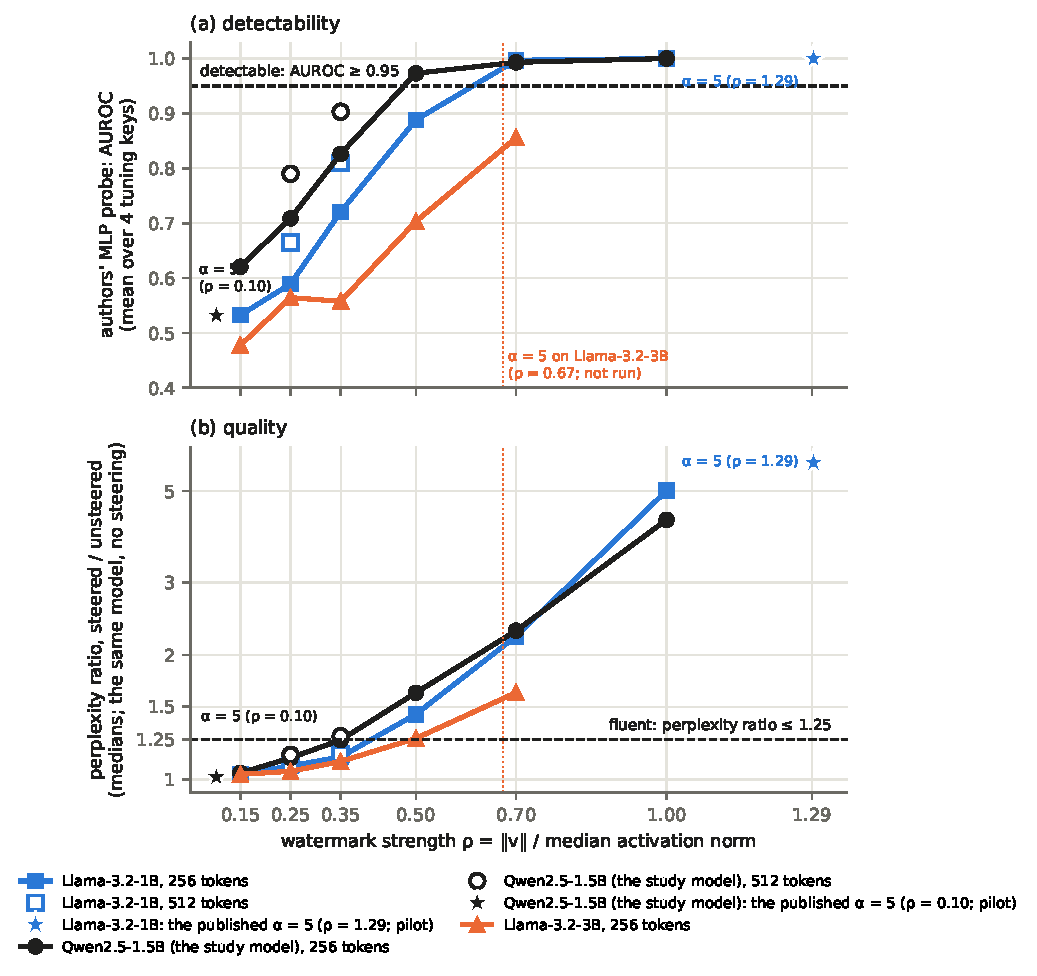
\includegraphics[width=0.8\textwidth,keepaspectratio]{figures/F1.pdf}
\caption{\textbf{Figure 1.} Calibration on three base models at 256 tokens: (a) the trained probe's AUROC and (b) the perplexity ratio to unsteered text against the strength \ensuremath{\rho}, with the 0.95 and 1.25 bars and the published \ensuremath{\alpha} = 5 marked as \ensuremath{\rho} for each model; 512-token points for two models. No model crosses both bars at the same \ensuremath{\rho}.}
\end{figure}

{\scriptsize\setlength{\tabcolsep}{1.5pt}\begin{longtable}[]{@{}
  >{\raggedright\arraybackslash}p{(\columnwidth - 14\tabcolsep) * \real{0.1200}}
  >{\raggedright\arraybackslash}p{(\columnwidth - 14\tabcolsep) * \real{0.0914}}
  >{\raggedright\arraybackslash}p{(\columnwidth - 14\tabcolsep) * \real{0.1314}}
  >{\raggedright\arraybackslash}p{(\columnwidth - 14\tabcolsep) * \real{0.1486}}
  >{\raggedright\arraybackslash}p{(\columnwidth - 14\tabcolsep) * \real{0.1200}}
  >{\raggedright\arraybackslash}p{(\columnwidth - 14\tabcolsep) * \real{0.1486}}
  >{\raggedright\arraybackslash}p{(\columnwidth - 14\tabcolsep) * \real{0.1486}}
  >{\raggedright\arraybackslash}p{(\columnwidth - 14\tabcolsep) * \real{0.0914}}@{}}
\caption{\textbf{Table 2.} Calibration of the published scheme on three base models with strength measured as \ensuremath{\rho} (tuning keys 9001--9004; 40 test texts per key; the reproduction pilot's \ensuremath{\alpha} = 5 rows as \ensuremath{\rho}): no strength is both probe-detectable and perplexity-neutral}\tabularnewline
\toprule\noalign{}
\begin{minipage}[b]{\linewidth}\raggedright
model (base)
\end{minipage} & \begin{minipage}[b]{\linewidth}\raggedright
tokens
\end{minipage} & \begin{minipage}[b]{\linewidth}\raggedright
\ensuremath{\rho} = \ensuremath{\|}v\ensuremath{\|} / N
\end{minipage} & \begin{minipage}[b]{\linewidth}\raggedright
\ensuremath{\alpha} equivalent
\end{minipage} & \begin{minipage}[b]{\linewidth}\raggedright
authors' MLP probe AUROC (mean over 4 tuning keys)
\end{minipage} & \begin{minipage}[b]{\linewidth}\raggedright
perplexity ratio (steered / unsteered, medians)
\end{minipage} & \begin{minipage}[b]{\linewidth}\raggedright
detectable (AUROC \ensuremath{\geq} 0.95)
\end{minipage} & \begin{minipage}[b]{\linewidth}\raggedright
fluent (ratio \ensuremath{\leq} 1.25)
\end{minipage} \\
\midrule\noalign{}
\endfirsthead
\toprule\noalign{}
\begin{minipage}[b]{\linewidth}\raggedright
model (base)
\end{minipage} & \begin{minipage}[b]{\linewidth}\raggedright
tokens
\end{minipage} & \begin{minipage}[b]{\linewidth}\raggedright
\ensuremath{\rho} = \ensuremath{\|}v\ensuremath{\|} / N
\end{minipage} & \begin{minipage}[b]{\linewidth}\raggedright
\ensuremath{\alpha} equivalent
\end{minipage} & \begin{minipage}[b]{\linewidth}\raggedright
authors' MLP probe AUROC (mean over 4 tuning keys)
\end{minipage} & \begin{minipage}[b]{\linewidth}\raggedright
perplexity ratio (steered / unsteered, medians)
\end{minipage} & \begin{minipage}[b]{\linewidth}\raggedright
detectable (AUROC \ensuremath{\geq} 0.95)
\end{minipage} & \begin{minipage}[b]{\linewidth}\raggedright
fluent (ratio \ensuremath{\leq} 1.25)
\end{minipage} \\
\midrule\noalign{}
\endhead
\bottomrule\noalign{}
\endlastfoot
Llama-3.2-1B & 256 & 0.15 & 0.6 & 0.53 & 1.03 & no & yes \\
Llama-3.2-1B & 256 & 0.25 & 1.0 & 0.59 & 1.08 & no & yes \\
Llama-3.2-1B & 256 & 0.35 & 1.4 & 0.72 & 1.13 & no & yes \\
Llama-3.2-1B & 256 & 0.50 & 1.9 & 0.89 & 1.44 & no & no \\
Llama-3.2-1B & 256 & 0.70 & 2.7 & 1.00 & 2.22 & yes & no \\
Llama-3.2-1B & 256 & 1.00 & 3.9 & 1.00 & 5.00 & yes & no \\
Llama-3.2-1B & 512 & 0.25 & 1.0 & 0.66 & 1.09 & no & yes \\
Llama-3.2-1B & 512 & 0.35 & 1.4 & 0.81 & 1.15 & no & yes \\
Llama-3.2-1B & 256 & published \ensuremath{\alpha} = 5 \ensuremath{\rightarrow} \ensuremath{\rho} = 1.29 & 5.0 & 1.00 (pilot; best detector 1.00) & 5.85 (median perplexity 32.6 vs 5.6) & yes & no \\
Qwen2.5-1.5B & 256 & 0.15 & 7.4 & 0.62 & 1.04 & no & yes \\
Qwen2.5-1.5B & 256 & 0.25 & 12.3 & 0.71 & 1.13 & no & yes \\
Qwen2.5-1.5B & 256 & 0.35 & 17.2 & 0.83 & 1.25 & no & yes \\
Qwen2.5-1.5B & 256 & 0.50 & 24.5 & 0.97 & 1.62 & yes & no \\
Qwen2.5-1.5B & 256 & 0.70 & 34.3 & 0.99 & 2.29 & yes & no \\
Qwen2.5-1.5B & 256 & 1.00 & 49.0 & 1.00 & 4.25 & yes & no \\
Qwen2.5-1.5B & 512 & 0.25 & 12.3 & 0.79 & 1.15 & no & yes \\
Qwen2.5-1.5B & 512 & 0.35 & 17.2 & 0.90 & 1.27 & no & no \\
Qwen2.5-1.5B & 256 & published \ensuremath{\alpha} = 5 \ensuremath{\rightarrow} \ensuremath{\rho} = 0.10 & 5.0 & 0.53 (pilot; best detector 0.57) & 1.01 (median perplexity 5.5 vs 5.5) & no & yes \\
Llama-3.2-3B & 256 & 0.15 & 1.1 & 0.48 & 1.03 & no & yes \\
Llama-3.2-3B & 256 & 0.25 & 1.9 & 0.56 & 1.05 & no & yes \\
Llama-3.2-3B & 256 & 0.35 & 2.6 & 0.56 & 1.11 & no & yes \\
Llama-3.2-3B & 256 & 0.50 & 3.7 & 0.70 & 1.26 & no & no \\
Llama-3.2-3B & 256 & 0.70 & 5.2 & 0.86 & 1.62 & no & no \\
Llama-3.2-3B & 256 & published \ensuremath{\alpha} = 5 \ensuremath{\rightarrow} \ensuremath{\rho} \ensuremath{\approx} 0.67 (not run; nearest grid point 0.70) & 5.0 & --- & --- & --- & --- \\
\end{longtable}}

\emph{N is the median token activation norm at the steered layer over unsteered text (Llama-3.2-1B: layer 8 of 16, N = 5.67; Qwen2.5-1.5B: layer 14 of 28, N = 56.90; Llama-3.2-3B: layer 14 of 28, N = 12.67). The operating-point rule (the smallest \ensuremath{\rho} with AUROC \ensuremath{\geq} 0.95 and ratio \ensuremath{\leq} 1.25) returned none on every model at either length. Perplexity is the continuation's under the same model without steering, given the prompt; the pilot's perplexity column was added after that pilot's rule was fixed (exploratory).}

This is a result under our conditions, not a test of the authors' claim. They report ``no quality degradation'' (p.~1) on instruction-tuned models at 512 tokens, by a DeBERTa quality classifier and MMLU, with perplexity moving from 7.62 to 8.06 on Llama-3.1-8B and from 9.76 to 8.27 on Llama-3.2-1B (Table 7, p.~15) \citep{ardoin2026selfrecognition}; we measured base models, continuation-only perplexity under the same model, our prompts, our probe training and four tuning keys. The negative result is also the probe's, not the watermark's: the exact test of Section 3 later attributed 97.5\% of genuine texts at \(\rho = 0.25\) (Section 5.3), where the perplexity ratio is 1.13. The attacks therefore run along the curve, \(\rho \in \{0.25, 0.35, 0.50, 0.70\}\), rather than at one setting.

\hypertarget{forging-the-trained-probe-without-the-key}{%
\subsection{Forging the trained probe without the key}\label{forging-the-trained-probe-without-the-key}}

Study 1 asks whether a passive attacker with the open weights and \(n \leq \text{1,024}\) watermarked texts, and no detector access, can make the owner's probe accept new text, in three locked versions whose rules Table 1 lists (v0.4, with the repetition term on both sides, is the primary result). The probe's threshold held on the owner's null texts (pooled false-positive rate 1.4\%, G1) but flagged 3.6\% of the human continuations of the same prompts, and the watermark worked by the probe's own standard (genuine acceptance \(\geq 20\)\%, L1) only at \(\rho \geq 0.35\) (8.0\% at \(\rho = 0.25\), which is descriptive in Study 1).

\textbf{Route A recovers nothing.} The activation-mean estimator (Section 2.3) never approached the key: the median cosine over the 8 keys stayed at or below 0.16 at every strength and budget up to \(n = \text{1,024}\), with the steered layer found for at most 3 of 8 keys at any budget (R1 fails at every level; Table A15; the full grid in Table A14). At \(\rho = 0.35\) its v0.4 forgeries are \textbf{not practical} (upper bounds 11.5 and 10.0\% against a bar of 14.3\%); at 0.50 and 0.70 the verdict is \textbf{inconclusive}, because the per-key rates are bimodal: at \(\rho = 0.70\) the median FA is 73.0\% but its lower bound 8.5\% (App. D).

\textbf{Route B forges without the key.} Footprint imitation at the attacker's chosen layer was accepted by the probe at every working strength from \(n = 64\) texts, at 42.5--100.0\% against genuine rates of 32.0--100.0\% (R2 practical at \(n = 64\) at \(\rho = 0.35\), 0.50 and 0.70), although its vector has a median cosine of at most 0.062 with the key (Table 3). Many of those texts were degenerate: steering at the first layers gave broken text the probe still accepted, and under v0.3's perplexity-only condition most of Route B's accepted texts at \(\rho = 0.70\) were loops (exploratory readings; Table A15; App. E). With both conditions on both sides, the pre-registered v0.4 verdicts are: \textbf{Route B is practical at \(\rho = 0.35\)} (FA 19.5 {[}7.0, 35.0{]}\% at \(n = 256\) against a bar of 14.3\%, its lower bound above the random key's upper bound of 3.5\%), and \textbf{inconclusive at 0.50 and 0.70}, where the probe accepts at least 99.0\% of its texts but only 26--54\% pass the fluency bars, so quality rather than detection limits the forgery (Figure 2). Generic steering alone never suffices (F3 no at every level). At \(\rho = 0.35\) the watermark itself is weak by this detector (genuine texts accepted and fluent 28.5\% of the time) and the bar is strict, those texts being close to unsteered text; at \(\rho = 0.70\) the same relative bar is lenient, the genuine texts being themselves degraded, and one forgery that passed both bars read as word salad (exploratory; App. E).

\begin{figure}[htbp]
\centering
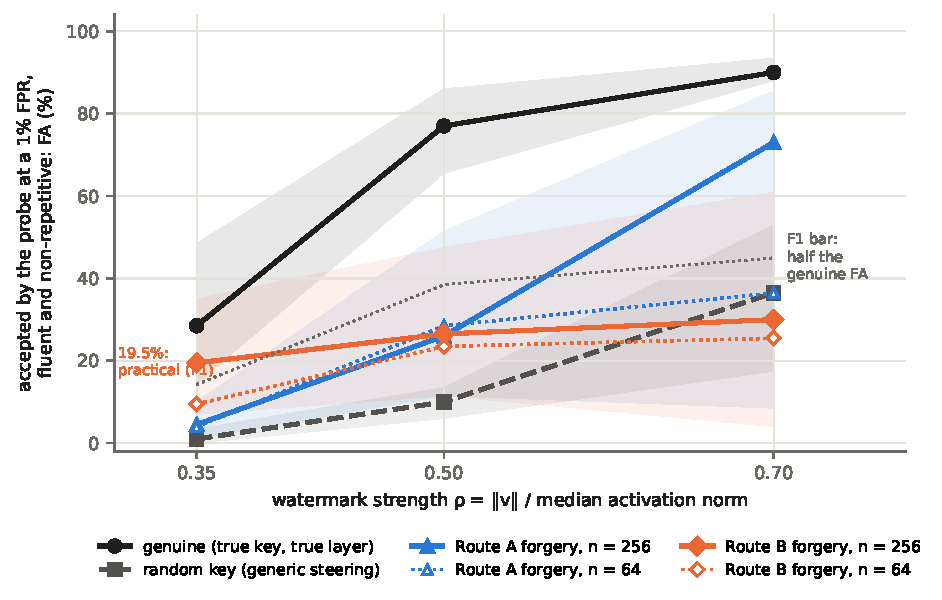
\includegraphics[width=0.8\textwidth,keepaspectratio]{figures/F2.pdf}
\caption{\textbf{Figure 2.} Fluent, non-repetitive acceptance by the owner's probe at its 1\% threshold against \ensuremath{\rho} for the genuine texts, the random-key control and the Route A and Route B forgeries at n = 64 and 256 (medians over 8 keys with 95\% cluster-bootstrap bands; the dashed bar is half the genuine rate, rule F1).}
\end{figure}

{\scriptsize\setlength{\tabcolsep}{1.5pt}\begin{longtable}[]{@{}
  >{\raggedright\arraybackslash}p{(\columnwidth - 14\tabcolsep) * \real{0.0529}}
  >{\raggedright\arraybackslash}p{(\columnwidth - 14\tabcolsep) * \real{0.1640}}
  >{\raggedright\arraybackslash}p{(\columnwidth - 14\tabcolsep) * \real{0.1640}}
  >{\raggedright\arraybackslash}p{(\columnwidth - 14\tabcolsep) * \real{0.1376}}
  >{\raggedright\arraybackslash}p{(\columnwidth - 14\tabcolsep) * \real{0.1217}}
  >{\raggedright\arraybackslash}p{(\columnwidth - 14\tabcolsep) * \real{0.0847}}
  >{\raggedright\arraybackslash}p{(\columnwidth - 14\tabcolsep) * \real{0.1640}}
  >{\raggedright\arraybackslash}p{(\columnwidth - 14\tabcolsep) * \real{0.1111}}@{}}
\caption{\textbf{Table 3.} Forging the owner's trained probe without the key (Study 1 v0.2 and v0.4; medians over 8 keys)}\tabularnewline
\toprule\noalign{}
\begin{minipage}[b]{\linewidth}\raggedright
\ensuremath{\rho}
\end{minipage} & \begin{minipage}[b]{\linewidth}\raggedright
texts
\end{minipage} & \begin{minipage}[b]{\linewidth}\raggedright
v0.2 R2 verdict (plain acceptance)
\end{minipage} & \begin{minipage}[b]{\linewidth}\raggedright
v0.2 plain acceptance at n = 64 / 256 / 1,024 (\%)
\end{minipage} & \begin{minipage}[b]{\linewidth}\raggedright
v0.4 FA at n = 64 / 256 (\%) {[}95\% CI{]}
\end{minipage} & \begin{minipage}[b]{\linewidth}\raggedright
F1 bar: half the oracle FA (\%)
\end{minipage} & \begin{minipage}[b]{\linewidth}\raggedright
v0.4 F1 verdict
\end{minipage} & \begin{minipage}[b]{\linewidth}\raggedright
Route vector's cosine with the key (v0.4, n = 256)
\end{minipage} \\
\midrule\noalign{}
\endfirsthead
\toprule\noalign{}
\begin{minipage}[b]{\linewidth}\raggedright
\ensuremath{\rho}
\end{minipage} & \begin{minipage}[b]{\linewidth}\raggedright
texts
\end{minipage} & \begin{minipage}[b]{\linewidth}\raggedright
v0.2 R2 verdict (plain acceptance)
\end{minipage} & \begin{minipage}[b]{\linewidth}\raggedright
v0.2 plain acceptance at n = 64 / 256 / 1,024 (\%)
\end{minipage} & \begin{minipage}[b]{\linewidth}\raggedright
v0.4 FA at n = 64 / 256 (\%) {[}95\% CI{]}
\end{minipage} & \begin{minipage}[b]{\linewidth}\raggedright
F1 bar: half the oracle FA (\%)
\end{minipage} & \begin{minipage}[b]{\linewidth}\raggedright
v0.4 F1 verdict
\end{minipage} & \begin{minipage}[b]{\linewidth}\raggedright
Route vector's cosine with the key (v0.4, n = 256)
\end{minipage} \\
\midrule\noalign{}
\endhead
\bottomrule\noalign{}
\endlastfoot
0.25 & oracle (true key, true layer); descriptive, L1 fails & --- & 8.0 / --- / --- & --- & --- & watermark not working (L1) & --- \\
0.35 & oracle (true key, true layer) & --- & 32.0 / --- / --- & 28.5 {[}14.5, 48.5{]} & --- & ceiling & --- \\
0.35 & random key (generic steering) & --- & 1.5 / --- / --- & 1.0 {[}0.0, 3.5{]} & --- & F3 generic steering suffices: no & --- \\
0.35 & Route A: key recovery (activation mean) & inconclusive & 11.0 / 3.5 / 4.5 & 4.0 {[}1.0, 11.5{]} / 4.5 {[}1.0, 10.0{]} & 14.3 & not practical & 0.079 \\
0.35 & Route B: footprint imitation & practical (n=64) & 42.5 / 56.0 / 45.5 & 9.5 {[}1.5, 24.0{]} / 19.5 {[}7.0, 35.0{]} & 14.3 & practical (n=256) & 0.047 \\
0.5 & oracle (true key, true layer) & --- & 86.0 / --- / --- & 77.0 {[}65.5, 86.0{]} & --- & ceiling & --- \\
0.5 & random key (generic steering) & --- & 13.0 / --- / --- & 10.0 {[}6.0, 13.5{]} & --- & F3 generic steering suffices: no & --- \\
0.5 & Route A: key recovery (activation mean) & not practical & 23.0 / 20.0 / 20.5 & 28.5 {[}11.0, 52.5{]} / 26.0 {[}11.5, 51.5{]} & 38.5 & inconclusive & 0.052 \\
0.5 & Route B: footprint imitation & practical (n=64) & 99.0 / 99.5 / 100.0 & 23.5 {[}11.0, 46.0{]} / 26.5 {[}11.5, 47.5{]} & 38.5 & inconclusive & 0.042 \\
0.7 & oracle (true key, true layer) & --- & 100.0 / --- / --- & 90.0 {[}88.0, 93.5{]} & --- & ceiling & --- \\
0.7 & random key (generic steering) & --- & 55.5 / --- / --- & 36.5 {[}17.5, 53.0{]} & --- & F3 generic steering suffices: no & --- \\
0.7 & Route A: key recovery (activation mean) & not practical & 80.5 / 90.5 / 89.0 & 36.5 {[}7.5, 76.5{]} / 73.0 {[}8.5, 85.5{]} & 45.0 & inconclusive & 0.000 \\
0.7 & Route B: footprint imitation & practical (n=64) & 100.0 / 100.0 / 100.0 & 25.5 {[}1.0, 70.5{]} / 30.0 {[}4.0, 61.0{]} & 45.0 & inconclusive & 0.062 \\
\end{longtable}}

\emph{Plain acceptance: the probe accepts the text at its 1\% threshold (v0.2's rule). FA (v0.4's rule): accepted and no less fluent and no more repetitive than the key's own genuine watermarked texts (perplexity and seq-rep-4 at most their 95th percentiles). F1 practical: at some n the median FA reaches half the oracle's and its lower bound exceeds the random key's upper bound; not practical: both n's upper bounds fall below the bar; otherwise inconclusive. v0.2's R2 uses plain acceptance with the same practical clause. The random-key row's verdict is F3.}

\textbf{Reading.} We read these results as consistent with the probe detecting steering rather than the key (an inference): it accepts texts steered at other layers and in other directions, accepts degenerate text, and flags human text above its nominal rate. The scheme's authors note the related effect that ``paraphrasing human text acts as a spoofing mechanism for our detector'' (p.~5) \citep{ardoin2026selfrecognition}, and the finding concerns the detector type as we re-implemented and re-trained it on Qwen2.5-1.5B at 256 tokens, not their deployed models. The claim that survives the pre-registered rules is narrow: on this model, at the one strength where quality is acceptable (\(\rho = 0.35\)), a passive attacker with 256 outputs and no key produces fluent, non-repetitive text that the probe accepts at more than half the genuine rate.

\hypertarget{the-exact-test-detects-the-key-and-rejects-those-forgeries}{%
\subsection{The exact test detects the key and rejects those forgeries}\label{the-exact-test-detects-the-key-and-rejects-those-forgeries}}

Study 3 re-scores Study 1's texts with the exact key test S4 (Section 3) on the same 8 keys and strengths, with the probe's numbers from Study 1 beside it on the same texts (Table 4; Figure 3). Calibration first: the pooled false-positive rate on 8 keys \ensuremath{\times} 1,000 of the owner's unwatermarked texts was 0.81\% (G1), every key was calibrated at 0.1--1.7\% (G2), and the rate on human continuations was 0.68\% (H1; highest key 1.6\%), where the probe had flagged 3.6\%. The test is exact on average over keys (Section 3); G2 is what makes it usable with one key, and on these keys it passed.

\begin{figure}[htbp]
\centering
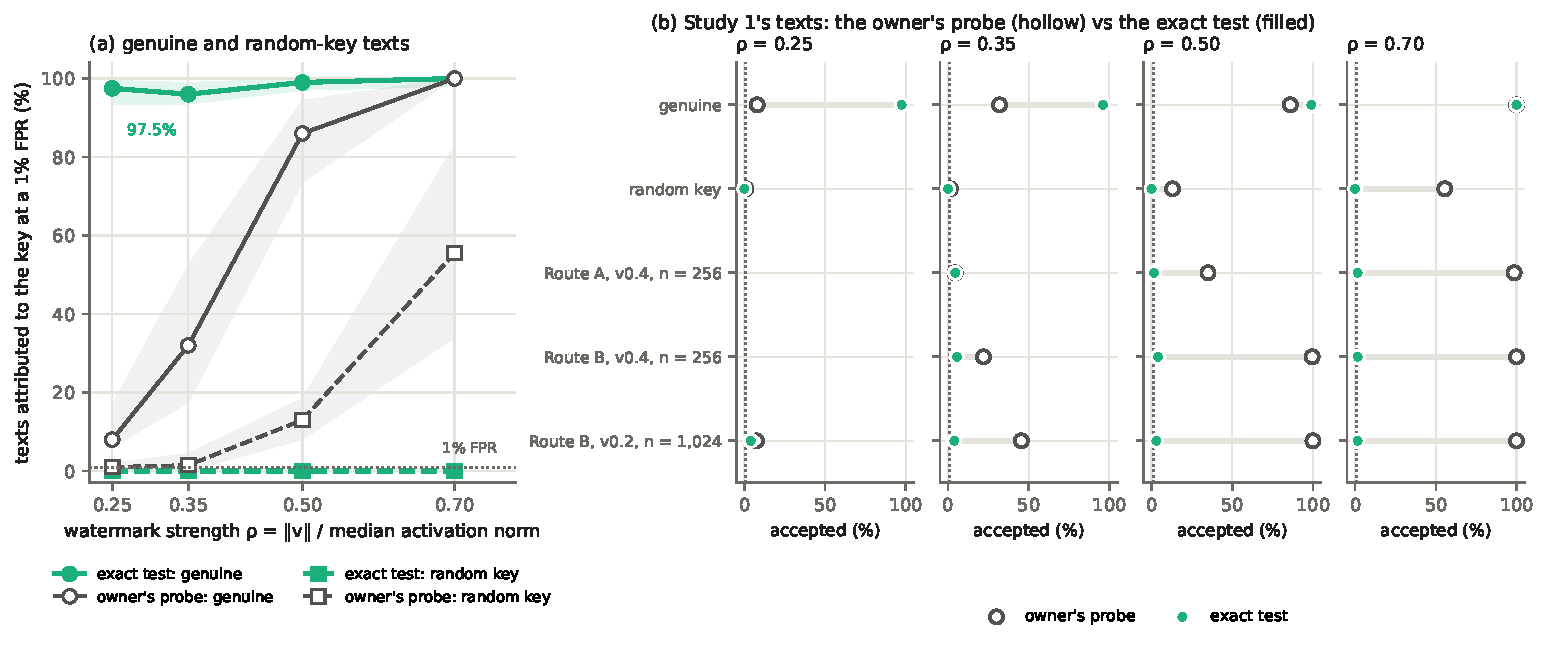
\includegraphics[width=0.8\textwidth,keepaspectratio]{figures/F3.pdf}
\caption{\textbf{Figure 3.} (a) Genuine and random-key texts attributed at an exact 1\% false-positive rate by the exact test and by the probe, against \ensuremath{\rho}. (b) Study 1's texts accepted by the probe (hollow) and attributed by the exact test (filled), per forgery set and strength.}
\end{figure}

{\scriptsize\setlength{\tabcolsep}{1.5pt}\begin{longtable}[]{@{}
  >{\raggedright\arraybackslash}p{(\columnwidth - 20\tabcolsep) * \real{0.0422}}
  >{\raggedright\arraybackslash}p{(\columnwidth - 20\tabcolsep) * \real{0.1224}}
  >{\raggedright\arraybackslash}p{(\columnwidth - 20\tabcolsep) * \real{0.0549}}
  >{\raggedright\arraybackslash}p{(\columnwidth - 20\tabcolsep) * \real{0.1097}}
  >{\raggedright\arraybackslash}p{(\columnwidth - 20\tabcolsep) * \real{0.1224}}
  >{\raggedright\arraybackslash}p{(\columnwidth - 20\tabcolsep) * \real{0.0759}}
  >{\raggedright\arraybackslash}p{(\columnwidth - 20\tabcolsep) * \real{0.1013}}
  >{\raggedright\arraybackslash}p{(\columnwidth - 20\tabcolsep) * \real{0.0970}}
  >{\raggedright\arraybackslash}p{(\columnwidth - 20\tabcolsep) * \real{0.0759}}
  >{\raggedright\arraybackslash}p{(\columnwidth - 20\tabcolsep) * \real{0.1097}}
  >{\raggedright\arraybackslash}p{(\columnwidth - 20\tabcolsep) * \real{0.0886}}@{}}
\caption{\textbf{Table 4.} The exact key test (S4) on the study keys: detection, random-key attribution and Study 1's forgeries re-scored (medians over 8 keys; 256-token texts; p \ensuremath{\leq} 0.01 with 999 null keys)}\tabularnewline
\toprule\noalign{}
\begin{minipage}[b]{\linewidth}\raggedright
\ensuremath{\rho}
\end{minipage} & \begin{minipage}[b]{\linewidth}\raggedright
genuine texts attributed, exact test (\%) {[}95\% CI{]}
\end{minipage} & \begin{minipage}[b]{\linewidth}\raggedright
the probe on the same texts (\%)
\end{minipage} & \begin{minipage}[b]{\linewidth}\raggedright
E1: exact \ensuremath{-} probe, points {[}95\% CI{]}: verdict
\end{minipage} & \begin{minipage}[b]{\linewidth}\raggedright
random-key texts attributed: exact / probe (\%)
\end{minipage} & \begin{minipage}[b]{\linewidth}\raggedright
genuine at p \ensuremath{\leq} 0.001 (\%)
\end{minipage} & \begin{minipage}[b]{\linewidth}\raggedright
v0.4 Route A, n = 256: exact FA (\%) {[}95\% CI{]} (probe FA)
\end{minipage} & \begin{minipage}[b]{\linewidth}\raggedright
v0.4 Route B, n = 256: exact FA (\%) {[}95\% CI{]} (probe FA)
\end{minipage} & \begin{minipage}[b]{\linewidth}\raggedright
X1 bar: half the genuine exact FA (\%)
\end{minipage} & \begin{minipage}[b]{\linewidth}\raggedright
X1 verdicts
\end{minipage} & \begin{minipage}[b]{\linewidth}\raggedright
X3 generic steering suffices
\end{minipage} \\
\midrule\noalign{}
\endfirsthead
\toprule\noalign{}
\begin{minipage}[b]{\linewidth}\raggedright
\ensuremath{\rho}
\end{minipage} & \begin{minipage}[b]{\linewidth}\raggedright
genuine texts attributed, exact test (\%) {[}95\% CI{]}
\end{minipage} & \begin{minipage}[b]{\linewidth}\raggedright
the probe on the same texts (\%)
\end{minipage} & \begin{minipage}[b]{\linewidth}\raggedright
E1: exact \ensuremath{-} probe, points {[}95\% CI{]}: verdict
\end{minipage} & \begin{minipage}[b]{\linewidth}\raggedright
random-key texts attributed: exact / probe (\%)
\end{minipage} & \begin{minipage}[b]{\linewidth}\raggedright
genuine at p \ensuremath{\leq} 0.001 (\%)
\end{minipage} & \begin{minipage}[b]{\linewidth}\raggedright
v0.4 Route A, n = 256: exact FA (\%) {[}95\% CI{]} (probe FA)
\end{minipage} & \begin{minipage}[b]{\linewidth}\raggedright
v0.4 Route B, n = 256: exact FA (\%) {[}95\% CI{]} (probe FA)
\end{minipage} & \begin{minipage}[b]{\linewidth}\raggedright
X1 bar: half the genuine exact FA (\%)
\end{minipage} & \begin{minipage}[b]{\linewidth}\raggedright
X1 verdicts
\end{minipage} & \begin{minipage}[b]{\linewidth}\raggedright
X3 generic steering suffices
\end{minipage} \\
\midrule\noalign{}
\endhead
\bottomrule\noalign{}
\endlastfoot
0.25 & 97.5 {[}93.5, 99.5{]} & 8.0 & +86.0 {[}+80.5, +90.0{]}: exact test more powerful & 0.0 / 1.0 & 85.0 & --- (no v0.4 forgeries at 0.25) & --- & 44.0 & --- & no \\
0.35 & 96.0 {[}93.5, 99.0{]} & 32.0 & +62.0 {[}+46.0, +78.0{]}: exact test more powerful & 0.0 / 1.5 & 93.0 & 4.5 {[}0.0, 14.0{]} (probe 4.5) & 4.5 {[}1.5, 8.0{]} (probe 19.5) & 43.2 & A: not practical; B: not practical & no \\
0.5 & 99.0 {[}97.0, 100.0{]} & 86.0 & +13.5 {[}+3.0, +25.5{]}: exact test more powerful & 0.0 / 13.0 & 98.5 & 1.5 {[}0.0, 32.5{]} (probe 26.0) & 3.5 {[}0.0, 9.5{]} (probe 26.5) & 45.0 & A: not practical; B: not practical & no \\
0.7 & 100.0 {[}98.0, 100.0{]} & 100.0 & +0.0 {[}-2.0, +0.0{]}: no clear difference & 0.0 / 55.5 & 98.0 & 1.0 {[}0.0, 22.0{]} (probe 73.0) & 1.0 {[}0.0, 4.0{]} (probe 30.0) & 45.0 & A: not practical; B: not practical & no \\
\end{longtable}}

\emph{Calibration: pooled false-positive rate 0.81\% on 8 keys \ensuremath{\times} 1,000 unwatermarked model texts (G1; range 0.3--2.5); every key calibrated at 0.1--1.7\% (G2 bar 3\%); 0.68\% on 1,000 human continuations (H1; highest key 1.6\%); at p \ensuremath{\leq} 0.001 with 9,999 null keys 0.11\% on model text and 0.05\% on human text. Exact FA: attributed by the exact test and fluent by v0.4's definition. X1 and X3 have the form of v0.4's F1 and F3 with the exact test in place of the probe. The probe's numbers are Study 1's, on the same texts.}

\textbf{Detection.} The exact test attributed 97.5, 96.0, 99.0 and 100.0\% of genuine 256-token texts at \(\rho = 0.25\), 0.35, 0.50 and 0.70 (medians over 8 keys; P1 passes at every level), against the probe's 8.0, 32.0, 86.0 and 100.0\% on the same texts; the paired differences are +86.0 {[}+80.5, +90.0{]}, +62.0 {[}+46.0, +78.0{]} and +13.5 {[}+3.0, +25.5{]} points at the three lower strengths (E1: the exact test more powerful) and +0.0 {[}-2.0, +0.0{]} at \(\rho = 0.70\) (no clear difference). Random-key texts, the generic-steering control, were attributed to the key 0.0\% of the time at every strength (X3: no everywhere), where the probe accepted up to 55.5\% of them at \(\rho = 0.70\).

\textbf{Forgeries.} Scored by the exact test with v0.4's fluency conditions, Study 1's forgeries are \textbf{not practical for the median key at \(\rho = 0.35\), 0.50 and 0.70, for both routes} (X1): their exact fluent acceptance is 0.0--4.5\% against bars of 43.2--45.0\%, half the genuine exact FA. The one practical probe forgery, Route B at \(\rho = 0.35\) and \(n = 256\) with a probe FA of 19.5\%, reaches 4.5\% under the exact test; Route A at \(\rho = 0.70\), at a probe FA of 73.0\%, reaches 1.0\%. Figure 3(b) shows the pattern over Study 1's text sets: the probe's acceptance of forgeries rises with \(\rho\) towards 100\%, the exact test's stays near the 1\% line.

\textbf{Per-key leakage (descriptive).} The median hides where forgeries do pass. Over the 384 key \ensuremath{\times} strength \ensuremath{\times} forgery-set cells, 35 have exact acceptance of 50\% or more, and acceptance rises with the attacker's recovered cosine (Spearman 0.68 for Route A and 0.56 for Route B over all cells; App. D). Route A's forgeries pass mainly for the keys it partly recovered at high strength; some Route B forgeries pass at a cosine near zero, which we read as the copied footprint reproducing enough of that key's effect on the output distribution for the gradient test to see (an inference). That steering directions differ in detectability and quality cost is noted by the scheme's authors (p.~7) \citep{ardoin2026selfrecognition}; it is why per-key tables accompany every median (App. D).

Two consequences carry forward. Against these passive forgers with \(n \leq \text{1,024}\) texts, the exact test keeps the watermark's value as provenance evidence for the median key, with more power at low strength, a false-positive rate checked per key and no acceptance of generic steering for the median key: a deployer should test the key, not the steering. And the protection is only as good as the key's secrecy, since where an attack recovered much of the key its forgeries passed. Whether the key stays secret is Section 5.4.

\hypertarget{the-detectors-statistic-steals-the-fixed-key-from-64-texts}{%
\subsection{The detector's statistic steals the fixed key from 64 texts}\label{the-detectors-statistic-steals-the-fixed-key-from-64-texts}}

Study 5's gate P0 ran the attack that Section 3 predicts: Route A\ensuremath{'} averages the exact test's own standardised gradient over the attacker's \(n\) observed texts, re-encoded through the open weights, and reads the key off the mean (Section 2.3; App. C). On the study keys it is \textbf{practical at \(n = 64\) at \(\rho = 0.35\) and 0.50} (Table 6; Figure 4). From 64 texts the median cosine with the key is 0.940 at \(\rho = 0.35\) and 0.951 at 0.50 when the layer is given, and 0.932 and 0.920 when the attacker searches all 28 layers, which finds layer 14 for 6 of 8 keys at \(\rho = 0.35\) and 6 of 8 at 0.50. Its fluent forgeries, made with the known-layer estimate, are then attributed as often as the owner's genuine texts: FA 88.0 {[}76.5, 93.0{]}\% against a genuine 86.5 {[}83.5, 90.5{]}\% at \(\rho = 0.35\), and 85.5 {[}82.5, 90.0{]}\% against 90.0 {[}87.0, 92.5{]}\% at 0.50, with the random-key control at 0.0 {[}0.0, 0.5{]}\%; with the layer-search estimate, from 256 texts, they are attributed 86.0 {[}81.5, 90.5{]}\% at \(\rho = 0.35\) and 87.5 {[}80.5, 93.0{]}\% at 0.50 (App. C.3). More texts change little (85.0\% and 87.5\% at \(n = \text{1,024}\); every key between 78 and 93\% at 0.50). Study 1's activation-mean estimator recovered nothing from the same 1,024 texts (median cosine \(\leq 0.16\); Section 5.2); the test's statistic recovers the key from 64.

\begin{figure}[htbp]
\centering
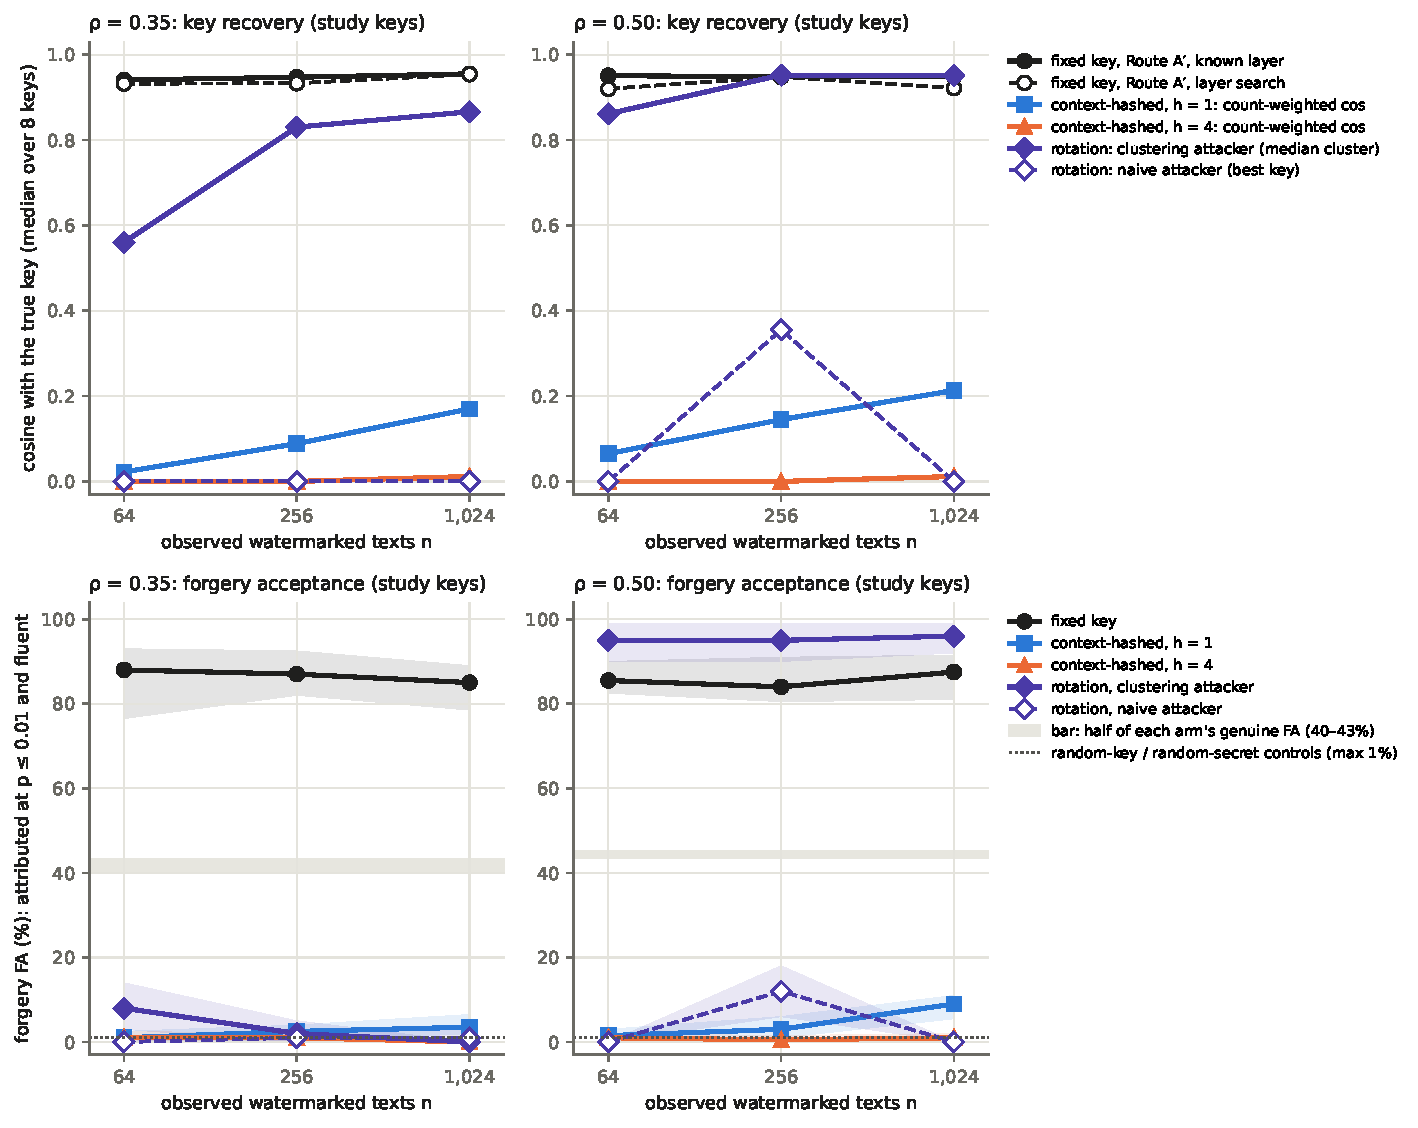
\includegraphics[width=0.8\textwidth,keepaspectratio]{figures/F4.pdf}
\caption{\textbf{Figure 4.} Key recovery (cosine with the true key) and forgery acceptance against the attacker's budget n at \ensuremath{\rho} = 0.35 and 0.50: the fixed key (Route A\ensuremath{'} at the known layer and with the layer search), the context-hashed arms and rotation (the naive and clustering attackers), with the D1 bars and the random-key controls.}
\end{figure}

{\scriptsize\setlength{\tabcolsep}{1.5pt}\begin{longtable}[]{@{}
  >{\raggedright\arraybackslash}p{(\columnwidth - 14\tabcolsep) * \real{0.1337}}
  >{\raggedright\arraybackslash}p{(\columnwidth - 14\tabcolsep) * \real{0.0495}}
  >{\raggedright\arraybackslash}p{(\columnwidth - 14\tabcolsep) * \real{0.1287}}
  >{\raggedright\arraybackslash}p{(\columnwidth - 14\tabcolsep) * \real{0.1980}}
  >{\raggedright\arraybackslash}p{(\columnwidth - 14\tabcolsep) * \real{0.1535}}
  >{\raggedright\arraybackslash}p{(\columnwidth - 14\tabcolsep) * \real{0.1040}}
  >{\raggedright\arraybackslash}p{(\columnwidth - 14\tabcolsep) * \real{0.0891}}
  >{\raggedright\arraybackslash}p{(\columnwidth - 14\tabcolsep) * \real{0.1436}}@{}}
\caption{\textbf{Table 6.} The fixed key and the keyed arms under the gradient-averaging attacker: detection and stealing against the budget (Study 5; medians over 8 keys; rotation's forgery sets have no per-key structure and are means)}\tabularnewline
\toprule\noalign{}
\begin{minipage}[b]{\linewidth}\raggedright
arm and attacker
\end{minipage} & \begin{minipage}[b]{\linewidth}\raggedright
\ensuremath{\rho}
\end{minipage} & \begin{minipage}[b]{\linewidth}\raggedright
genuine detection, P1 (\%)
\end{minipage} & \begin{minipage}[b]{\linewidth}\raggedright
key recovery at n = 64 / 256 / 1,024 (cosine with the key; count-weighted for the hashed arms)
\end{minipage} & \begin{minipage}[b]{\linewidth}\raggedright
forgery FA at n = 64 / 256 / 1,024 (\%) {[}95\% CI{]}
\end{minipage} & \begin{minipage}[b]{\linewidth}\raggedright
bar: half the genuine FA (\%)
\end{minipage} & \begin{minipage}[b]{\linewidth}\raggedright
control FA (\%) {[}95\% CI{]}
\end{minipage} & \begin{minipage}[b]{\linewidth}\raggedright
verdict
\end{minipage} \\
\midrule\noalign{}
\endfirsthead
\toprule\noalign{}
\begin{minipage}[b]{\linewidth}\raggedright
arm and attacker
\end{minipage} & \begin{minipage}[b]{\linewidth}\raggedright
\ensuremath{\rho}
\end{minipage} & \begin{minipage}[b]{\linewidth}\raggedright
genuine detection, P1 (\%)
\end{minipage} & \begin{minipage}[b]{\linewidth}\raggedright
key recovery at n = 64 / 256 / 1,024 (cosine with the key; count-weighted for the hashed arms)
\end{minipage} & \begin{minipage}[b]{\linewidth}\raggedright
forgery FA at n = 64 / 256 / 1,024 (\%) {[}95\% CI{]}
\end{minipage} & \begin{minipage}[b]{\linewidth}\raggedright
bar: half the genuine FA (\%)
\end{minipage} & \begin{minipage}[b]{\linewidth}\raggedright
control FA (\%) {[}95\% CI{]}
\end{minipage} & \begin{minipage}[b]{\linewidth}\raggedright
verdict
\end{minipage} \\
\midrule\noalign{}
\endhead
\bottomrule\noalign{}
\endlastfoot
fixed key (h = 0), Route A\ensuremath{'} & 0.35 & 96.0 & 0.94 / 0.95 / 0.95 & 88.0 {[}76.5, 93.0{]} / 87.0 {[}82.0, 92.5{]} / 85.0 {[}78.5, 89.0{]} & 43.2 (genuine FA 86.5) & 0.0 {[}0.0, 0.5{]} & P0: practical (n=64) \\
context-hashed, h = 1 & 0.35 & 92.5 & 0.02 / 0.09 / 0.17 & 1.0 {[}0.0, 2.5{]} / 2.5 {[}0.0, 4.0{]} / 3.5 {[}2.0, 6.5{]} & 42.0 (genuine FA 84.0) & 1.0 {[}0.0, 1.5{]} & D1: stealing blocked at n \textless= 1024 \\
context-hashed, h = 4 & 0.35 & 90.0 & 0.00 / 0.00 / 0.01 & 1.0 {[}0.0, 2.5{]} / 1.0 {[}0.0, 2.0{]} / 0.0 {[}0.0, 0.0{]} & 40.0 (genuine FA 80.0) & 0.5 {[}0.0, 1.5{]} & D1: stealing blocked at n \textless= 1024 \\
rotation (K = 8), naive attacker & 0.35 & 93.0 (union test; told the key: 96.0) & 0.00 / 0.00 / 0.00 (best cos with any key) & 0.0 {[}0.0, 0.0{]} / 1.0 {[}0.0, 3.0{]} / 1.0 {[}0.0, 3.0{]} & 43.2 (the fixed key's genuine FA) & 0.0 {[}0.0, 0.5{]} & D1: stealing blocked at n \textless= 1024 \\
rotation (K = 8), clustering attacker & 0.35 & as above & 4 of 8 keys (forging cluster cos 0.31) / 6 of 8 keys (forging cluster cos 0.00) / 6 of 8 keys (forging cluster cos 0.00) & 8.0 {[}3.0, 14.0{]} / 2.0 {[}0.0, 5.0{]} / 0.0 {[}0.0, 0.0{]} & 43.2 & 0.0 {[}0.0, 0.5{]} & D1: stealing blocked at n \textless= 1024 \\
fixed key (h = 0), Route A\ensuremath{'} & 0.5 & 99.0 & 0.95 / 0.95 / 0.95 & 85.5 {[}82.5, 90.0{]} / 84.0 {[}80.5, 91.0{]} / 87.5 {[}81.0, 91.5{]} & 45.0 (genuine FA 90.0) & 0.0 {[}0.0, 0.5{]} & P0: practical (n=64) \\
context-hashed, h = 1 & 0.5 & 96.5 & 0.07 / 0.14 / 0.21 & 1.5 {[}0.0, 3.0{]} / 3.0 {[}1.0, 6.0{]} / 9.0 {[}5.5, 11.0{]} & 44.0 (genuine FA 88.0) & 1.0 {[}0.0, 1.0{]} & D1: stealing blocked at n \textless= 1024 \\
context-hashed, h = 4 & 0.5 & 95.5 & 0.00 / 0.00 / 0.01 & 1.0 {[}0.0, 2.0{]} / 0.5 {[}0.0, 1.5{]} / 1.0 {[}0.0, 2.0{]} & 43.8 (genuine FA 87.5) & 0.5 {[}0.0, 1.5{]} & D1: stealing blocked at n \textless= 1024 \\
rotation (K = 8), naive attacker & 0.5 & 98.5 (union test; told the key: 99.0) & 0.00 / 0.36 / 0.00 (best cos with any key) & 0.0 {[}0.0, 0.0{]} / 12.0 {[}6.0, 18.0{]} / 0.0 {[}0.0, 0.0{]} & 45.0 (the fixed key's genuine FA) & 0.0 {[}0.0, 0.5{]} & D1: stealing blocked at n \textless= 1024 \\
rotation (K = 8), clustering attacker & 0.5 & as above & 7 of 8 keys (forging cluster cos 0.95) / 8 of 8 keys (forging cluster cos 0.96) / 8 of 8 keys (forging cluster cos 0.96) & 95.0 {[}90.0, 99.0{]} / 95.0 {[}90.0, 99.0{]} / 96.0 {[}92.0, 99.0{]} & 45.0 & 0.0 {[}0.0, 0.5{]} & D1: practical (n=64) \\
\textbf{post hoc, labelled (App. G):} rotation, clustering attacker, forging with every cluster & 0.35 & as above & n = 256: 7 clusters with cos \ensuremath{\geq} 0.5; the study's rule picked cos 0.00 & n = 256: best cluster 96; largest cluster 88; the study's rule 1 & 43.2 & --- & 7 of 7 recovered clusters reach the bar (not pre-registered; the D1 verdict stands) \\
\textbf{post hoc, labelled (App. G):} rotation, clustering attacker, forging with every cluster & 0.35 & as above & n = 1,024: 6 clusters with cos \ensuremath{\geq} 0.5; the study's rule picked cos 0.00 & n = 1,024: best cluster 90; largest cluster 89; the study's rule 1 & 43.2 & --- & 5 of 6 recovered clusters reach the bar (not pre-registered; the D1 verdict stands) \\
\end{longtable}}

\emph{FA: attributed at p \ensuremath{\leq} 0.01 (the keyed test for the hashed arms; the union test for rotation) and fluent by the arm's own genuine texts' bars. P0 and D1: practical at the first n where the FA reaches the bar with its lower bound above the control's upper bound; otherwise stealing blocked at n \ensuremath{\leq} 1,024. The control is a random key (fixed arm, rotation) or a random secret (hashed arms). The last two rows are the labelled post-hoc addendum (not pre-registered); the pre-registered rotation verdict at \ensuremath{\rho} = 0.35 stands as written.}

This is the measured fact behind the paper's central inference (Section 3): the gradient the owner projects on the key to detect it is, averaged over outputs, an estimator of the key, so the detector's statistic is also the best estimator among those we tested (Section 2.3). Two bounds go with it. The budget comparison with token-level stealing carries an access caveat: our attacker needs 64 texts of 256 tokens, 16,384 tokens in all, where the token-level attacks use 30,000 responses, 2.2 million tokens or 2,000 texts (Section 2.2) \citep{jovanovic2024stealing, pang2024nofreelunch, zhang2026beyondseal}, but those attackers query a black-box API, and ours re-encodes the outputs through the model that produced them, which only the open weights allow. And the strength matters: on the tuning keys the pilot that motivated Study 5 reached a median cosine of 0.80 from 4 texts and 0.95 from 16 at \(\rho = 0.35\), but only 0.57 from 100 texts at \(\rho = 0.70\) (a pilot, labelled; Table A5), where the study keys were not attacked; at that strength the attack is weaker and untested.

\hypertarget{scrubbing-under-the-exact-test}{%
\subsection{Scrubbing under the exact test}\label{scrubbing-under-the-exact-test}}

Study 2 scrubs the fixed key's genuine texts and scores the result with the exact test at matched quality (Section 4; Table 5; Figure 5): 100 genuine texts per key and strength, paraphrased by P-Qwen and P-Phi with the attacker's self-check and up to three attempts, or edited at 5\% of the words by the true key (an insider bound), by the attacker's Route A estimate from Study 1, or at random. The test stayed calibrated on paraphrased null text (pooled false-positive rates 0.33\% and 0.44\%; every key at 0.0--0.6\% and 0.0--1.4\%) and attributed the unscrubbed originals at 96.0--100.0\%.

\begin{figure}[htbp]
\centering
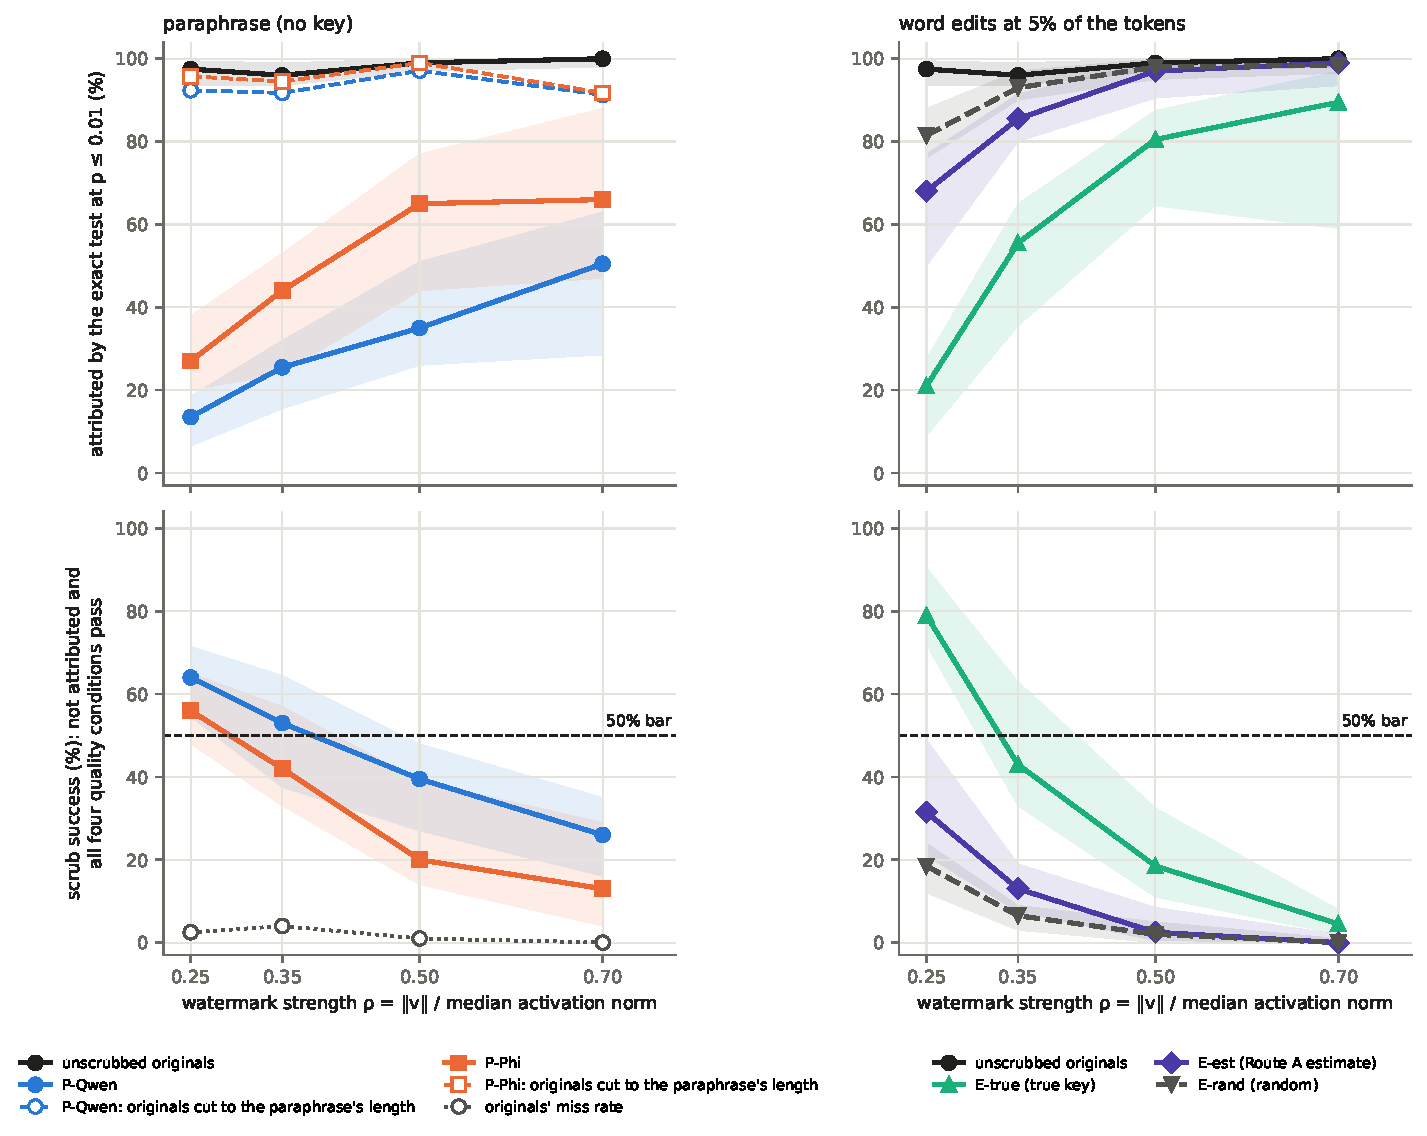
\includegraphics[width=0.8\textwidth,keepaspectratio]{figures/F5.pdf}
\caption{\textbf{Figure 5.} Detection after scrubbing (top) and scrub success (bottom) against \ensuremath{\rho} for the two paraphrasers, with the length-matched controls and the originals' miss rate, and for word edits at 5\% of the tokens with the true key, the attacker's estimate and random positions; the dashed line is the 50\% bar.}
\end{figure}

{\footnotesize\begin{longtable}[]{@{}
  >{\raggedright\arraybackslash}p{(\columnwidth - 12\tabcolsep) * \real{0.0704}}
  >{\raggedright\arraybackslash}p{(\columnwidth - 12\tabcolsep) * \real{0.1831}}
  >{\raggedright\arraybackslash}p{(\columnwidth - 12\tabcolsep) * \real{0.1479}}
  >{\raggedright\arraybackslash}p{(\columnwidth - 12\tabcolsep) * \real{0.1831}}
  >{\raggedright\arraybackslash}p{(\columnwidth - 12\tabcolsep) * \real{0.1268}}
  >{\raggedright\arraybackslash}p{(\columnwidth - 12\tabcolsep) * \real{0.0704}}
  >{\raggedright\arraybackslash}p{(\columnwidth - 12\tabcolsep) * \real{0.2183}}@{}}
\caption{\textbf{Table 5.} Scrubbing the fixed key's evidence under the exact test at matched quality (Study 2; medians over 8 keys; 100 genuine texts per key and strength)}\tabularnewline
\toprule\noalign{}
\begin{minipage}[b]{\linewidth}\raggedright
\ensuremath{\rho}
\end{minipage} & \begin{minipage}[b]{\linewidth}\raggedright
method
\end{minipage} & \begin{minipage}[b]{\linewidth}\raggedright
detected after (\%)
\end{minipage} & \begin{minipage}[b]{\linewidth}\raggedright
all four quality conditions pass (\%)
\end{minipage} & \begin{minipage}[b]{\linewidth}\raggedright
scrub success (\%) {[}95\% CI{]}
\end{minipage} & \begin{minipage}[b]{\linewidth}\raggedright
keys \ensuremath{\geq} 50\%
\end{minipage} & \begin{minipage}[b]{\linewidth}\raggedright
pre-registered verdict (comparator)
\end{minipage} \\
\midrule\noalign{}
\endfirsthead
\toprule\noalign{}
\begin{minipage}[b]{\linewidth}\raggedright
\ensuremath{\rho}
\end{minipage} & \begin{minipage}[b]{\linewidth}\raggedright
method
\end{minipage} & \begin{minipage}[b]{\linewidth}\raggedright
detected after (\%)
\end{minipage} & \begin{minipage}[b]{\linewidth}\raggedright
all four quality conditions pass (\%)
\end{minipage} & \begin{minipage}[b]{\linewidth}\raggedright
scrub success (\%) {[}95\% CI{]}
\end{minipage} & \begin{minipage}[b]{\linewidth}\raggedright
keys \ensuremath{\geq} 50\%
\end{minipage} & \begin{minipage}[b]{\linewidth}\raggedright
pre-registered verdict (comparator)
\end{minipage} \\
\midrule\noalign{}
\endhead
\bottomrule\noalign{}
\endlastfoot
0.25 & unscrubbed originals & 97.5 & --- & --- & --- & P1 pass \\
0.25 & P-Qwen paraphrase & 13.5 & 75.0 & 64.0 {[}54.5, 71.5{]} & 7 of 8 & S1 effective (originals' miss 2.5 {[}0.5, 6.5{]}) \\
0.25 & P-Phi paraphrase & 27.0 & 83.0 & 56.0 {[}48.0, 65.0{]} & 7 of 8 & S1 effective (originals' miss 3.0 {[}0.0, 6.0{]}) \\
0.25 & E-true: 5\% edits, true key & 21.0 & 99.0 & 79.0 {[}72.0, 90.5{]} & 8 of 8 & S2 effective \\
0.25 & E-est: 5\% edits, Route A estimate & 68.0 & 99.0 & 31.5 {[}21.0, 49.0{]} & 2 of 8 & S2 not effective \\
0.25 & E-rand: 5\% edits, random & 81.5 & 99.5 & 18.5 {[}12.0, 24.0{]} & 0 of 8 & C1 E-est \ensuremath{-} E-rand: +14.5 {[}+5.0, +28.0{]}: the estimate helps \\
0.35 & unscrubbed originals & 96.0 & --- & --- & --- & P1 pass \\
0.35 & P-Qwen paraphrase & 25.5 & 74.0 & 53.0 {[}37.5, 64.5{]} & 5 of 8 & S1 effective (originals' miss 4.0 {[}1.0, 6.5{]}) \\
0.35 & P-Phi paraphrase & 44.0 & 79.0 & 42.0 {[}33.0, 57.0{]} & 2 of 8 & S1 inconclusive (originals' miss 3.0 {[}0.0, 7.0{]}) \\
0.35 & E-true: 5\% edits, true key & 55.5 & 98.0 & 43.0 {[}33.0, 63.0{]} & 3 of 8 & S2 inconclusive \\
0.35 & E-est: 5\% edits, Route A estimate & 85.5 & 98.5 & 13.0 {[}7.5, 19.0{]} & 0 of 8 & S2 not effective \\
0.35 & E-rand: 5\% edits, random & 93.0 & 99.0 & 6.5 {[}3.0, 9.0{]} & 0 of 8 & C1 E-est \ensuremath{-} E-rand: +6.5 {[}+2.0, +11.0{]}: the estimate helps \\
0.5 & unscrubbed originals & 99.0 & --- & --- & --- & P1 pass \\
0.5 & P-Qwen paraphrase & 35.0 & 64.0 & 39.5 {[}27.0, 48.0{]} & 1 of 8 & S1 not effective (originals' miss 1.0 {[}0.0, 3.0{]}) \\
0.5 & P-Phi paraphrase & 65.0 & 76.0 & 20.0 {[}14.0, 39.0{]} & 1 of 8 & S1 not effective (originals' miss 0.0 {[}0.0, 2.0{]}) \\
0.5 & E-true: 5\% edits, true key & 80.5 & 95.5 & 18.5 {[}11.0, 32.5{]} & 1 of 8 & S2 not effective \\
0.5 & E-est: 5\% edits, Route A estimate & 97.0 & 93.5 & 2.5 {[}0.5, 8.5{]} & 0 of 8 & S2 not effective \\
0.5 & E-rand: 5\% edits, random & 98.0 & 96.0 & 2.0 {[}0.0, 5.0{]} & 0 of 8 & C1 E-est \ensuremath{-} E-rand: +0.0 {[}-0.5, +7.0{]}: no clear difference \\
0.7 & unscrubbed originals & 100.0 & --- & --- & --- & P1 pass \\
0.7 & P-Qwen paraphrase & 50.5 & 49.5 & 26.0 {[}16.0, 35.0{]} & 1 of 8 & S1 not effective (originals' miss 0.0 {[}0.0, 2.0{]}) \\
0.7 & P-Phi paraphrase & 66.0 & 52.0 & 13.0 {[}4.0, 29.0{]} & 1 of 8 & S1 not effective (originals' miss 0.0 {[}0.0, 2.0{]}) \\
0.7 & E-true: 5\% edits, true key & 89.5 & 41.5 & 4.5 {[}2.0, 8.0{]} & 0 of 8 & S2 not effective \\
0.7 & E-est: 5\% edits, Route A estimate & 99.0 & 38.5 & 0.0 {[}0.0, 2.0{]} & 0 of 8 & S2 not effective \\
0.7 & E-rand: 5\% edits, random & 98.5 & 39.0 & 0.0 {[}0.0, 1.0{]} & 0 of 8 & C1 E-est \ensuremath{-} E-rand: +0.0 {[}-0.5, +0.0{]}: no clear difference \\
\end{longtable}}

\emph{Success: not attributed by the exact test at p \ensuremath{\leq} 0.01 and fluency, repetition, length and meaning within the owner's bars (\S{}4). S1 and S2: effective if the median success is at least 50\% and its lower bound exceeds the comparator's upper bound (the originals' miss rate for paraphrase; E-rand for the edits); not effective if the upper bound is below 50\%; otherwise inconclusive. C1 is the paired difference E-est \ensuremath{-} E-rand over keys. Calibration after paraphrase: pooled false-positive rate 0.33\% (P-Qwen) and 0.44\% (P-Phi) on 8 keys \ensuremath{\times} 1,000 paraphrased unwatermarked texts; every key calibrated (0.0--0.6\% and 0.0--1.4\%).}

\textbf{Paraphrase scrubs at the quality-acceptable strengths and not above them.} At \(\rho = 0.25\) both paraphrasers are \textbf{effective}: success 64.0 {[}54.5, 71.5{]}\% for P-Qwen and 56.0 {[}48.0, 65.0{]}\% for P-Phi against the originals' miss rates of 2.5 {[}0.5, 6.5{]}\% and 3.0 {[}0.0, 6.0{]}\%, with 7 and 7 of 8 keys at or above 50\%. At \(\rho = 0.35\) P-Qwen is \textbf{effective} (53.0 {[}37.5, 64.5{]}\%; 5 of 8 keys) and P-Phi \textbf{inconclusive} (42.0 {[}33.0, 57.0{]}\%). At \(\rho = 0.50\) and 0.70 \textbf{neither is effective} (P-Qwen 39.5 and 26.0\%; P-Phi 20.0 and 13.0\%; one key in each cell reaches 50\%). The evidence is removed, not shortened: the originals cut to the paraphrase's length are still attributed 91.2--99.0\% of the time. At high strength quality is the other half of success: the share of P-Qwen's paraphrases passing all four conditions falls to 49.5\% at \(\rho = 0.70\).

\textbf{The true key helps only where the watermark is weak.} Edits of 5\% of the words guided by the true key are \textbf{effective only at \(\rho = 0.25\)} (success 79.0 {[}72.0, 90.5{]}\%; all 8 keys), \textbf{inconclusive at 0.35} (43.0 {[}33.0, 63.0{]}\%) and not effective above (at 10\% of the words the key removes the evidence at a visible fluency cost; App. F). Edits guided by the attacker's Route A estimate are \textbf{never effective} (success 31.5\% at \(\rho = 0.25\), falling to 0.0\%), although they beat random edits at \(\rho = 0.25\) and 0.35 (C1: +14.5 {[}+5.0, +28.0{]} and +6.5 {[}+2.0, +11.0{]} points; the estimate helps) and not above.

Two secondary readings. The per-key false-positive rate disperses after paraphrase: over 1,000 fresh keys of the public distribution the mean stays at 1.02\% and 0.94\% (exact on average), but 7.8\% and 6.5\% of keys exceed 3\% (maxima 22.6\% and 19.5\%), so a deployer should check their own key on paraphrased null text, the practical form of Section 3's ``on average over keys'' caveat. And the owner's trained probe accepts most of the same paraphrases at \(\rho \geq 0.50\) where the exact test does not, which we record as a lead, not a result (App. F). The comparison with the authors' robustness figures is indirect: their detector, models, paraphraser and metric differ, and their Table 3 reports attribution accuracy between two steered variants rather than detection against human text at a fixed false-positive rate \citep{ardoin2026selfrecognition}.

\hypertarget{keyed-directions-context-hashing-and-rotation-as-transfers}{%
\subsection{Keyed directions: context hashing and rotation, as transfers}\label{keyed-directions-context-hashing-and-rotation-as-transfers}}

Study 5 transfers two token-level defences to activation steering: keying the direction by the previous \(h\) tokens, the context hashing of Kirchenbauer et al. \citep{kirchenbauer2023watermark, kirchenbauer2024reliability}, and rotating among \(K\) keys with a union test, the multiple-key design of the same authors \citep{kirchenbauer2023watermark} as studied by Pang et al.~and Gu et al. \citep{pang2024nofreelunch, gu2024learnability} and deployed by SynthID-Text \citep{dathathri2024synthid}; both were named as future work by the scheme's authors (p.~7) \citep{ardoin2026selfrecognition}. The arms are \(h = 1\), \(h = 4\) and rotation among \(K = 8\) keys, beside the fixed key, at \(\rho = 0.35\) and 0.50 with the same 8 keys, against the attacker of Section 5.4 adapted to each arm (per observable context for the hashed arms; on the whole mixture, the naive attacker, or per cluster, the clustering attacker, for rotation; App. C) at \(n \in \{64, 256, \text{1,024}\}\), with Study 2's paraphrase pipeline for the robustness cost. The gates passed (pooled false-positive rates 0.83, 0.95 and 1.00\%; every key calibrated) and the keyed tests attributed 90.0--96.5\% of their genuine texts, the union test 93.0 and 98.5\% (P1; Table 6).

\textbf{Stealing (D1).} Both hashed arms \textbf{block this attacker at \(n \leq \text{1,024}\)}: the per-context attacker's forgeries are attributed at most 9.0\% (medians; upper bounds at most 11.0\%) against bars of 40--44\%, half the arms' genuine FA (Table 6; Figure 4); its per-context estimates stay poor (count-weighted cosine 0.213 for \(h = 1\) at \(n = \text{1,024}\), \(\rho = 0.50\); App. C). The verdict is bounded by the budget, not by the scheme: \(h = 1\)'s acceptance rises with \(n\) at \(\rho = 0.50\) (1.5 \ensuremath{\rightarrow} 3.0 \ensuremath{\rightarrow} 9.0\%), and the token-level literature steals context-hashed schemes with tens of thousands of responses (Section 2.2). Rotation blocks the naive attacker at both strengths but \textbf{falls to the clustering attacker at \(\rho = 0.50\), practical at \(n = 64\)}: it separates the mixture into the keys (7 of 8 recovered at cosine \(\geq 0.5\) from 64 texts, 8 of 8 from 256) and the union test attributes 95--96\% of its forgeries. At \(\rho = 0.35\) the pre-registered verdict is \textbf{stealing blocked at \(n \leq \text{1,024}\)}, and it stands as written; its reason is the attacker's pre-set rule for choosing the forging cluster, which at \(n = 256\) and 1,024 picked an outlier cluster with cosine 0.000 to every key while the other clusters recovered 6 of 8. A post-hoc addendum, labelled and not pre-registered (App. G; the last rows of Table 6; the hollow marker in Figure 6), forged with every cluster in turn: the best cluster's forgeries are attributed 96\% at \(n = 256\) and 90\% at \(n = \text{1,024}\), and 5 of the 6 recovered clusters reach the bar. Read with the pre-registered result, rotation among 8 keys multiplies this attacker's cost by about \(K\) against averaging and by nothing against clustering, at both strengths.

\begin{figure}[htbp]
\centering
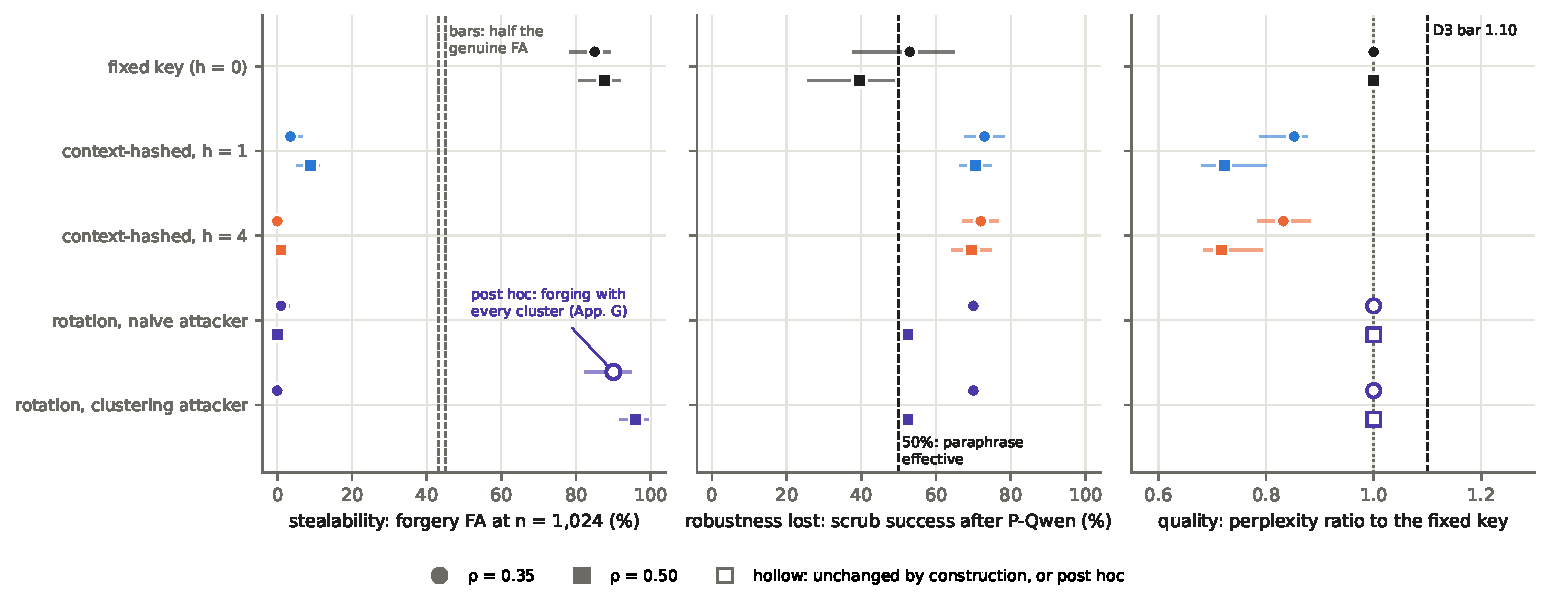
\includegraphics[width=0.8\textwidth,keepaspectratio]{figures/F6.pdf}
\caption{\textbf{Figure 6.} The frontier per arm at \ensuremath{\rho} = 0.35 and 0.50: forgery acceptance at n = 1,024 (stealability), scrub success after P-Qwen (robustness lost) and the perplexity ratio to the fixed key (quality), with the materiality bars. Rotation's clustering point at \ensuremath{\rho} = 0.35 is shown twice: the pre-registered rule's value and the addendum's every-cluster value (hollow, post hoc).}
\end{figure}

\textbf{Robustness (D2).} The hashed arms lose most of the paraphrase robustness the fixed key has (Table A16; Figure 6). After P-Qwen with the attacker's self-check, scrub success is 73.0 and 70.5\% against \(h = 1\) and 72.0 and 69.5\% against \(h = 4\), where the fixed key on the same prompts and keys was scrubbed 53.0 and 39.5\% of the time (Section 5.5). The paired differences are \textbf{material} for \(h = 1\) at both strengths (+22.0 {[}+6.0, +36.5{]} and +32.0 {[}+21.0, +44.0{]} points) and for \(h = 4\) at \(\rho = 0.50\) (+32.5 {[}+19.0, +45.5{]}), and \textbf{inconclusive} for \(h = 4\) at \(\rho = 0.35\) (+18.0 {[}+7.5, +33.5{]}: the median falls under the 20-point bar although the interval excludes zero). Attribution after paraphrase falls to 1.0--4.0\% for the keyed arms against the fixed key's 25.5 and 35.0\%: a paraphrase changes most contexts, so the content shift that survives it no longer lines up with any per-context key the owner can test (an inference; the same mechanism denies the attacker a stable direction to average). Rotation keeps the fixed key's robustness: the union test's loss on Study 2's paraphrases is +15.0 {[}+9.5, +18.5{]} and +13.0 {[}+8.5, +17.5{]} points, \textbf{immaterial} by the 20-point bar.

\textbf{Quality (D3).} Context keying costs nothing by our proxy and improves it, with perplexity ratios to the fixed key's texts on the same prompts of 0.72--0.85 (medians; no key above the 1.10 bar; \textbf{immaterial} everywhere), which is an improvement by that measure and not a quality claim (Section 4); rotation's quality is unchanged by construction.

\textbf{The point of difference with the token-level evidence.} That evidence on multiple keys is mixed (Section 6); our rotation result sits with Jovanovi\'c et al.'s \citep{jovanovic2024stealing} under this access model rather than with Pang et al.'s \citep{pang2024nofreelunch}, whose removal attack is untested here, so the no-free-lunch trade-off transfers only in this form: the context-width trade-off between stealing and paraphrase robustness reappears, rotation buys a constant factor against averaging and nothing against clustering, and immunity is claimed for no arm.

\hypertarget{the-trade-off-read-across-the-studies}{%
\subsection{The trade-off, read across the studies}\label{the-trade-off-read-across-the-studies}}

Read together, the studies describe one curve for the fixed key on this model (an interpretation, labelled; Figure 6). The strengths at which the exact test detects the key and paraphrase fails to scrub it, \(\rho \geq 0.50\), cost perplexity (ratios 1.62 and 2.29 against unsteered text; Section 5.1); the strengths with acceptable perplexity, \(\rho \leq 0.35\), are scrubbed by an off-the-shelf paraphrase (Section 5.5). The published probe fails the detectability criterion at the low strengths and is forgeable without the key at 0.35 (Section 5.2); the exact test rescues detection at every strength (Section 5.3), but its own statistic steals the fixed key from 64 texts (Section 5.4). Context keying moves the stealing corner at the price of the robustness corner; rotation keeps robustness and quality and falls to clustering (Section 5.6). That watermark designs trade robustness, quality and security against one another is the token-level literature's main theme \citep{pang2024nofreelunch, shen2025seek, jovanovic2024stealing} and is noted by the scheme's authors (p.~2) \citep{ardoin2026selfrecognition}; the contribution here is the measured curve along \(\rho\) for this family, on one model and against one attacker family.

\hypertarget{related-work}{%
\section{Related work}\label{related-work}}

\textbf{Stealing, forgery and scrubbing of token-level watermarks.} Jovanovi\'c et al. \citep{jovanovic2024stealing} define stealing as ``the act of reverse-engineering a watermark by querying the API of the watermarked LLM'' (p.~1), with a black-box attacker (p.~3) and ``\(n = 30{,}000\) responses of token length \(\leq 800\)'' (p.~6), spoof and scrub KGW-style schemes from the same estimate, and find that ``the supposed tradeoff between spoofing and scrubbing robustness \ldots{} in fact does not hold'' (p.~9). Pang et al. \citep{pang2024nofreelunch} state the trade-offs as guidelines, ``Robust watermarks are inherently vulnerable to spoofing attacks and are not suitable as proof of content authenticity alone'' (p.~5) and more keys defend against stealing at a cost in removal robustness (p.~7), stealing from ``2.2 million tokens in total'' (p.~6). Gu et al. \citep{gu2024learnability} learn a watermark by distillation and conclude that ``watermarking should not be used to attribute provenance or blame to a specific LM'' (p.~2). Zhang et al. \citep{zhang2026beyondseal} steal with ``2,000 victim watermarked texts'' (p.~8); MarkSec \citep{li2026marksec} fixes the attack definitions we adopt (p.~3) and excludes model-parameter schemes by scope (p.~2); SEEK \citep{shen2025seek} calls the scrubbing--forgery trade-off ``widely acknowledged'' (p.~1) and moves its boundary at the token level; paraphrase as an attack on detectors is Krishna et al. \citep{krishna2023paraphrasing}. What remains: every attack in the evaluations cited is token-level and black-box, none touches an activation scheme, and our attacker's white-box re-encoding changes the budget in kind (Section 2.2); the provenance conclusion of Gu et al.~and Pang et al.~is drawn here for this family (Section 5.3), citing them.

\textbf{Context hashing, key rotation and their trade-offs.} Both transferred mechanisms originate with Kirchenbauer et al. \citep{kirchenbauer2023watermark}: green lists from ``a pseudorandom number generator seeded with previous tokens'' (p.~4), a leak at \(h = 1\) that brute force can exploit (p.~6), the robustness cost of large \(h\), ``attack amplification'' (p.~6), and the multiple-key design, ``have \(k > 1\) different hidden keys, and to randomly choose one for each generation. At detection time, we run \(k\) tests, one for each of the possible keys'' (p.~7), defended by the absence of bias when averaging over many generations (p.~7). Our rotation arm is this design transferred; our clustering attacker is the counter to that averaging argument. Kirchenbauer et al. \citep{kirchenbauer2024reliability} find that ``a small context width \(h\) provides the best robustness to machine paraphrasing'' (p.~21) while secrecy wants a large \(h\) or ``sufficiently many keys'' (p.~17), the trade-off our \(h = 1\) and \(h = 4\) arms reproduce at the activation level. SynthID-Text deploys both mechanisms \citep{dathathri2024synthid, huggingface2026synthidconfig} and names stealing, forgery and scrubbing as ``an area of ongoing research'' (p.~6). On multiple keys the token-level evidence is mixed: three keys cut Pang et al.'s stealing success from 91\% to 13\% (p.~6), while Jovanovi\'c et al.~kept forgery success of 0.68--0.81 with \(k = 2\)--4 keys switched per response (Table 14, p.~20), ``not a viable defense against our attacker'' (p.~20); Gu et al.~note the multiple-testing cost (pp.~19--20), and Zhang et al.~name random key selection as a defence with a detection cost (p.~18).

\textbf{Model-internal watermarks and keyed directions.} Self-Recognition \citep{ardoin2026selfrecognition} is the scheme analysed (Section 2.1); its security rests, by its authors' statement, on the secrecy of the vector and layer and is left to future work (p.~7), and they report that ``paraphrasing human text acts as a spoofing mechanism for our detector'' (p.~5) and that ``Some vectors induce more severe degradations in generation quality, while others are more easily detectable'' (p.~7), which our per-key tables bear out. SLAM \citep{harelcanada2026slam} steers public sparse-autoencoder features chosen per document by a keyed hash (p.~5), reads a document identifier at detection, reports that ``DIPPER reduces TPR to 12\%/10\% on 2B/9B'' (p.~7) and targets ``provenance attribution rather than tamper-proof cryptographic authentication'' (p.~2); the words stealing, spoofing, forgery and threat model do not occur in it. AWM \citep{aremu2026awm} fine-tunes a keyed Gaussian direction per layer to monitor harmful outputs and finds that ``attacks optimized against one surrogate key do not reliably transfer against other (independent) keys'' (p.~2) for an adaptive evader who ``cannot query the detector'' (p.~3): the nearest keyed-direction design, under a different threat. GaussMark \citep{block2025gaussmark} perturbs weights, needs them for detection, ``a significantly stronger access model'' (p.~19), and leaves its per-token-key variant untested (p.~48). What remains: no member of the family has a measured key-recovery or forgery result under an attacker who holds the weights, and the paraphrase and evasion figures that SLAM's and AWM's authors report are robustness measurements of their own schemes, not scrubbing evaluations at matched quality under a per-key-calibrated test; SLAM and AWM are untested here.

\textbf{Score tests and randomisation tests.} Our detector is GaussMark's score statistic \citep{block2025gaussmark, rao1948score} for an additive activation vector, with Monte Carlo p-values \citep{phipson2010permutation} from resampled sparse keys in place of the Gaussian null (Section 3). GaussMark's guarantees ``are valid for any fixed \(x \in \mathcal{X}\), but are marginalized over the key \(\xi\)'' (p.~11); the per-key calibration gate we add is a practice, not a theorem, and the dispersion of per-key false-positive rates after paraphrase (Section 5.5) is its reason. Concurrently and outside watermarking, Chen et al. \citep{chen2026subliminal} recover a known residual-stream steering vector from a steered model's outputs by distillation and report the first-order relation of Section 3 in their setting, the initial gradient ``point{[}s{]} toward \(F\Delta_T\) rather than \(\Delta_T\)'' (p.~1), which iterative optimisation then inverts; our Route A\ensuremath{'} (Section 5.4) is that first gradient, standardised and averaged over the observed outputs, with no inversion.

\textbf{Quality bars.} Self-Recognition's appendix observes that ``a highly repetitive, degenerate loop often yields low PPL'' (p.~14); SLAM scores quality on four axes (p.~8); MarkSec relies on a judge model with ``no independent human annotation'' (p.~8). Our conditions pair perplexity with a repetition term on both the attacker's and the evaluator's side, add length and meaning conditions for scrubbing, and read fixed samples (Section 2.2, Section 4, App. E); they remain proxies, and no human judgement was collected.

\hypertarget{limitations-and-future-work}{%
\section{Limitations and future work}\label{limitations-and-future-work}}

\textbf{What was measured, and on what.} Every claim is bounded to one scheme as re-implemented by us (Self-Recognition's construction, not its released weights or deployed detector), one base model (Qwen/Qwen2.5-1.5B, layer 14 of 28), 8 study keys drawn from the scheme's own sparse key distribution, 256-token continuations of news-like prompts, and the strengths \(\rho \in \{0.25, 0.35, 0.50, 0.70\}\) (Study 5: 0.35 and 0.50). Rates are medians over keys with cluster-bootstrap intervals, except rotation's forgery rates, which are means over one corpus (Section 5.6), and the per-key tables of Appendix D show that keys differ: one key is detected far less often than the others at the highest strength, a few keys leak through the exact test where most do not, and the keyed arms' robustness cost varies by tens of points across keys. Where a pre-registered rule did not reach a verdict we say so: fluent forgery of the probe at \(\rho = 0.50\) and \(0.70\), P-Phi paraphrase and true-key edits at \(0.35\), and the robustness cost of \(h = 4\) at \(0.35\) are inconclusive, not negative.

\textbf{The attackers and their budgets.} We tested three passive attacker families (Routes A, A\('\) and B; the per-context and clustering attackers of Section 5.6), each holding the open weights and at most \(n =\) 1,024 watermarked texts and none querying the detector. ``Stealing blocked at \(n \leq\) 1,024'' therefore means blocked for these attackers at this budget, not immunity: the \(h = 1\) arm's forgery acceptance rises with \(n\) (1.5 \ensuremath{\rightarrow} 3.0 \ensuremath{\rightarrow} 9.0\% at \(\rho = 0.50\)), and the token-level literature steals context-hashed schemes with far larger budgets under a different access model (Section 5.4). We did not test an attacker who knows the exact test and optimises against it, one who combines paraphrase with key-guided edits, one who queries the detector, the repeated-query removal attack that Pang et al. \citep{pang2024nofreelunch} run against multiple keys, or human editing. At \(\rho = 0.70\) the key-recovery attack was weaker on tuning keys and was not run on the study keys.

\textbf{Quality is a proxy.} Fluency and faithfulness are measured by perplexity under the unsteered model, a repetition term, length and embedding similarity, with samples read under pre-set rules (Appendix H); no human judgement was collected, and the scheme's own quality classifier and MMLU evaluation were not computed. Because the relative bar is lenient at the strongest watermark, where the genuine text is itself degraded (Appendix E), fluent acceptance at \(\rho = 0.70\) should not be read as high-quality forgery.

\textbf{The reproduction and the exactness statement.} The published strength did not reproduce \emph{under our conditions}: base rather than instruction-tuned models, continuation-only perplexity under the same model, our prompts and our probe training. The authors' numbers are beside ours in Section 5.1, and we draw no conclusion about their claims beyond those conditions. The exact test's level is exact on average over keys; the per-key gate held for these 8 keys on unparaphrased text, but after paraphrase 7.8--6.5\% of freshly drawn keys exceeded a 3\% false-positive rate (Section 5.5, Appendix D), which is why a deployer should check the one key it holds.

\textbf{Novelty is at the search level.} ``To our knowledge'' means that no attack on Self-Recognition, SLAM or AWM appeared in the citing papers, listings and repositories we searched through October 2026; search absence is not proof of novelty. SLAM-style and AWM-style designs were discussed, not tested.

\textbf{Future work.} Five studies were specified but not run and would complete the picture: a SLAM-style keyed feature-steering target under the same protocols (the planned Study 4); the \(h = 1\) acceptance curve beyond \(n =\) 1,024 texts, where the token-level budgets lie; the per-position form of the keyed test with \(h = 0\) on the study keys (measured so far on tuning keys only; Appendix G); Pang et al.'s removal attack against rotation; and the 8B scale at which the scheme's authors report their results. An adaptive attacker against the exact test, and a human or model-judged coherence rating in place of the perplexity proxies, are the two measurements whose absence most limits the conclusions above.

\hypertarget{reproducibility-ethics-and-disclosure}{%
\section{Reproducibility, ethics and disclosure}\label{reproducibility-ethics-and-disclosure}}

\textbf{Pre-registration and locks.} The 6 studies were run from protocols fixed and hashed before any outcome existed (locked between 2026-09-26 and 2026-10-02), together with every code file the run imports and every reused input; the runners re-hash these files and refuse to run on a mismatch. A correction became a new version with the earlier results kept (Study 1 v0.2, v0.3 and v0.4 are all reported), the pilots that fixed the designs were run on tuning keys that no study used, and the one post-hoc analysis is labelled wherever it appears (Section 5.6, Appendix G). Table 1 gives each study's lock date, hash prefix, commit and run time; Appendix A gives the full table and one paragraph per protocol.

\textbf{Code and data availability.} The protocols, lock files, validation reports, run manifests, result files and every script that generated a number, table or figure in this paper are released in a public repository (https://github.com/SHENSHENZYC/activation-watermark-security; code under the MIT licence, text and figures under CC BY 4.0), without model weights or the generated corpora. Prompts come from the C4 realnewslike validation shard \citep{raffel2020t5} (ODC-BY 1.0, under the Common Crawl terms): 8,580 usable units, of which 6,896 were available for development and 1,684 were held out behind a loader that refuses to open them, and were never used. A WikiText-103 set \citep{merity2017pointer} was frozen as a second domain and is used by none of the six studies. No article text is redistributed; the repository holds identifiers and hashes only. Models were pinned to a revision and hashed (Appendix A): Qwen2.5-1.5B (apache-2.0) \citep{qwen2024qwen25, qwen2024card15b}, the paraphrasers Qwen2.5-1.5B-Instruct (Apache-2.0) \citep{qwen2024card15binstruct} and Phi-3.5-mini-instruct (MIT) \citep{abdin2024phi3}, Llama-3.2-1B and 3B (Llama 3.2 Community Licence) \citep{grattafiori2024llama3} for calibration only, and all-mpnet-base-v2 (Apache-2.0) \citep{reimers2019sbert} for embedding similarity.

\textbf{Compute.} Everything ran on one Apple-silicon laptop (M5, 16 GB unified memory; PyTorch 2.14.0 on MPS). The six locked runs took 91.1 hours in total (22.4, 6.4, 6.5, 2.9, 26.6 and 26.3 h), plus the reproduction pilot, three calibrations and three design pilots; no cloud compute was used.

\textbf{Ethics.} The scheme analysed is a published research method, re-implemented from its paper and public code on open-weight models; no deployed system was attacked, no detector was queried, and no private data was used. The attacks measured are the removal and forgery attempts that evaluation guidance names (Appendix I), and the forgeries exist only as research artefacts: the generated corpora are not released, and the only generated texts in the repository are the samples quoted in Appendix H and in the study reports. Nothing here assesses any provider's deployment or compliance.

\textbf{Use of AI tools.} The text and code were drafted with an AI system under the author's direction, as stated in the acknowledgements after Section 9.

\hypertarget{conclusion}{%
\section{Conclusion}\label{conclusion}}

A deployer of an activation-steering watermark of this family learns four things from these studies, each bounded to one model, one layer, 8 keys, 256-token texts and a passive attacker with the open weights and at most 1,024 outputs. The published detector type, a trained probe, is forgeable without the key at the only strength where quality is acceptable, and, on our reading, it detects steering rather than the key (Section 5.2); testing the key directly with an exact, per-key-calibrated score test rescues detection at every strength and blocks those forgeries. That same statistic is the best estimator among those we tested, so the fixed key is recovered from 64 outputs at the known layer, or from 256 with a layer search, and forged, and an off-the-shelf paraphrase removes the evidence at the strengths with acceptable perplexity. Keying the direction by context, a transfer from token-level watermarking, stops that attacker at the budget tested at the price of most of the paraphrase robustness; rotating among keys keeps robustness and quality but buys only a constant factor against a clustering attacker (pre-registered at \(\rho = 0.50\), post hoc at 0.35). If such watermarks are to serve as the robust, reliable and secure provenance mechanisms that regulators now describe, they will need keyed verification tools whose false-positive rate is checked per key, and whose security is measured against the attacker who holds the weights.

\hypertarget{acknowledgements-and-use-of-ai-tools}{%
\subsection*{Acknowledgements and use of AI tools}\label{acknowledgements-and-use-of-ai-tools}}
\addcontentsline{toc}{subsection}{Acknowledgements and use of AI tools}

This work received no external funding. The text and code of this paper were drafted by Claude (Anthropic) under the author's direction and under the pre-registered protocols described in Section 4 and Appendix A; the author designed the studies, took every decision recorded in the project's decision log, revised every section, verified every number against the locked outputs and takes full responsibility for the content. Codex (OpenAI) assisted with the final review and revision; the author reviewed and approved the changes. No AI system is an author. The language models that are part of the method (the watermarked model and the two paraphrasers) are described in Section 4.

\bibliographystyle{plainnat}
\bibliography{references}

\appendix

\hypertarget{protocols-and-locks}{%
\section{Protocols and locks}\label{protocols-and-locks}}

Every study was run from a protocol fixed and hashed before any outcome existed (Table A1). This appendix gives one paragraph per protocol: the question, the rules, the materiality bars, the stop rules and what was not claimed, in the order the studies were run. The protocols themselves, the lock files, the validation reports and the run manifests are in the repository (\texttt{research/\allowbreak{}STUDY*\_\allowbreak{}PROTOCOL\_\allowbreak{}v*.\allowbreak{}md}, \texttt{research/\allowbreak{}outputs/\allowbreak{}\textless{}study\textgreater{}/\allowbreak{}PRE\_\allowbreak{}RUN\_\allowbreak{}LOCK.\allowbreak{}json}, \texttt{INPUT\_\allowbreak{}VALIDATION.\allowbreak{}json}, \texttt{RUN\_\allowbreak{}MANIFEST*.\allowbreak{}json}).

\textbf{The lock mechanism.} A protocol's status line is set to LOCKED, and the SHA-256 of the protocol, of every code file the run imports and of every reused input file (earlier studies' locked data and outputs, the prompt-set manifest, the model manifests) is written to \texttt{PRE\_\allowbreak{}RUN\_\allowbreak{}LOCK.\allowbreak{}json} with the git commit, the approval and an explicit statement that no outcome exists. The runner re-hashes everything before each phase and after the run and refuses to start if any hash differs; the input validation includes tamper tests of that refusal. Input validation runs on inputs only: synthetic data (planted signals detected, none otherwise; p-values uniform under a simulated null), the tuning keys, the owner's reference texts, timing against a pre-set budget, and a pipeline smoke test that asserts every result field the protocol lists is produced. The holdout prompt set is sealed in the loader, which raises without a \emph{final} lock; no lock in this paper is final, and the holdout remains sealed for follow-up work.

\textbf{Study 1 v0.1 (locked 2026-09-25; stopped at its gate).} Key recovery and spoofing against the fixed scheme with a training-free cosine detector at the published \(\alpha\). Gate G1 (a working watermark under that detector) failed on Qwen2.5-1.5B (detection 0\% on the 4 tuning keys at \(\alpha = 5\) and 0\% at \(\alpha = 10\)), and the study stopped as its protocol required. The reproduction pilot and three calibrations (fixed specifications on the tuning keys only) then established that the authors' detector is a trained probe, that raw \(\alpha\) does not transfer across models, and that no relative strength \(\rho\) on three 1--3B base models is both probe-detectable and perplexity-neutral at 256 or 512 tokens (Section 5.1). The follow-up pre-committed in that record is v0.2: attack along the trade-off curve.

\textbf{Study 1 v0.2 (locked 2026-09-26; 22.4 h; 7 code files hashed).} Question: with the open model and \(n\) watermarked texts, can an attacker identify \(l\) and estimate \(v\) (Q1a), and generate text the owner's probe accepts at a 1\% false-positive rate, and does that require the key (Q1b)? Keys 1001--1008 at \(\rho \in \{0.25, 0.35, 0.50, 0.70\}\) on layer 14. Gates: G1, the pooled false-positive rate on pool A2 within {[}0.3, 2.5{]}\%; G2, attack isolation asserted in code. Per-level gate L1: median oracle acceptance at least 20\%. Rules: R1, recovery succeeds at the smallest \(n\) with median \(\cos(\hat v, v) \geq 0.9\) and the layer found for at least 7 of 8 keys, fails at this budget if no \(n \leq \text{1,024}\) qualifies, partial if the median cosine at 1,024 is in {[}0.5, 0.9); R2, forgery is practical per route if at some \(n \leq 256\) the median acceptance is at least 50\% of the oracle's and its lower 95\% bound exceeds the random-key control's upper bound, not practical if the median at \(n = \text{1,024}\) is below \(\max(2 \times\) the random-key median, 2\%\()\), otherwise inconclusive; R3, generic steering suffices if the random-key median reaches 50\% of the oracle's. Materiality: forged texts accepted at half the genuine rate at a 1\% false-positive rate make the watermark unreliable as provenance evidence. Stop rules: G1 fails, or every level fails L1. Not claimed: the first stealing attack on LLM watermarks; security or insecurity of the family in general or at 8B scale; other models or schemes. Validation: 14/14 checks passed. The owner's detector is the public code's MLP as its configuration file sets it (commit \texttt{7c26938}): 4 hidden layers of widths 2048, 64, 64, 32 with ReLU, trained for one epoch on the owner's own texts; the paper's text describes ``two hidden layers of width 32'' (p.~3), so the implemented probe is the wider of the two.

\textbf{Study 1 v0.3 (locked 2026-09-27; 6.4 h; 243 v0.2 files reused read-only).} v0.2's rule R2 had no quality condition and an exploratory reading of its forgeries found many accepted texts to be gibberish. v0.3 asks Q1c: can a passive attacker who screens its own candidates for fluency forge texts that are both accepted and no less fluent than the owner's genuine texts? The attacker gains a five-candidate layer search with 16 trial generations per candidate on its own prompts, scored by continuation-only perplexity (it does not see the prompts behind the observed texts), keeping candidates within 1.2 times the observed texts' median. Metric FA: accepted and with perplexity at most the key-level oracle's 95th percentile. Rules F1 (practical, not practical, inconclusive, in R2's form with FA) and F3 (generic steering) at \(\rho \in \{0.35, 0.50, 0.70\}\), \(n \in \{64, 256\}\). An integrity check first re-scores v0.2's oracle texts with the reloaded probes (within \(10^{-4}\)); if it fails, the study stops. v0.2's verdicts stand. Validation: 14/14 checks passed.

\textbf{Study 1 v0.4 (locked 2026-09-28; 6.5 h).} v0.3's perplexity-only fluency rule admitted repetitive loops (an exploratory reading, labelled in its report). v0.4 asks v0.3's question with a repetition term on both sides, fixed before any v0.4 outcome: the attacker's self-check also requires at most 2 of 16 trials with seq-rep-4 above the observed texts' 95th percentile, and the evaluation's fluency requires seq-rep-4 at most the key-level oracle's 95th percentile. Rules F1 and F3 unchanged in form; secondaries re-score v0.2's and v0.3's forgeries under the new rule and record what the attacker's check chose. Validation includes the check that, with the repetition term switched off, v0.4's code reproduces v0.3's locked FA medians exactly. v0.4 is the paper's primary forgery result; v0.3 stays as the perplexity-only result and v0.2 as the plain-acceptance result. Validation: 17/17 checks passed.

\textbf{Study 3 (locked 2026-09-30; 2.9 h; 562 Study 1 files reused read-only).} The exact key test (Section 3) on Study 1's keys and texts, with no new generation: Q3a, does it detect genuine text at a 1\% false-positive rate and how does it compare with the probe on the same texts; Q3b, is its false-positive rate near 1\% for each fixed key, on model text and on human text; Q3c, does it accept Study 1's forgeries, which were made without the key and without knowledge of this test. Gates: G1, pooled false-positive rate on 8 keys \ensuremath{\times} 1,000 unwatermarked texts within {[}0.3, 2.5{]}\%; G2, a key is calibrated if its rate is at most 3.0\%, uncalibrated keys are excluded from the verdicts and reported, and fewer than 6 calibrated keys stops the study. Per-level gate P1: median oracle detection at least 20\%. Rules: X1 (forgery practical against the exact test, v0.4's F1 with the exact test in place of the probe), X3 (generic steering), E1 (power against the probe: the median paired difference in detection on the same 100 oracle texts per key, with a paired bootstrap interval). Secondaries: H1, the human-text rate; S3 (the unstandardised gradient) beside S4; \(p \leq 0.001\) with 9,999 null keys; probe-and-exact combinations; a key-leakage lens relating forgeries' acceptance to the attacker's recovered cosine. Not claimed: security against an attacker who adapts to the exact test; per-key exactness in general; novelty of the statistic. Validation: 10/10 checks passed.

\textbf{Study 2 (locked 2026-10-01; 26.6 h).} Scrubbing under the exact test at matched quality, on Study 1's genuine texts: Q2a, can an off-the-shelf paraphraser (P-Qwen; P-Phi on the first 50 texts of each key and strength) remove S4's evidence while keeping fluency, length and meaning; Q2b, how often do word edits of 5\% of the tokens remove it when steered by the true key (an insider bound), by the attacker's Study 1 estimate, or at random. Gates: G1 and G2 as Study 3 but on the \emph{paraphrased} null texts, per paraphraser; P1 as Study 3. Rules: S1, paraphrase is effective if the median success is at least 50\% and its lower bound exceeds the upper bound of the originals' miss rate, not effective if the upper bound is below 50\%, otherwise inconclusive; S2, the same for each key-guided edit arm against random edits of the same size; C1, whether the attacker's estimate helps (the paired difference E-est \ensuremath{-} E-rand). Materiality: success of 50\% means the watermark gives no provenance evidence for half of the typical key's texts at matched quality. Bounds checked at the extremes: the 50\% bar is absolute; if random edits alone reached it, the edit arms could not be effective and ``random edits suffice'' would be reported. Secondaries: the edit curve at 2 and 10\%; length-matched controls (each original truncated to its paraphrase's length and re-scored, to separate ``less text'' from ``evidence removed''); the probe on the same scrubs; per-key calibration after paraphrase for the study keys and for 1,000 fresh keys; stricter quality readings; samples read. Not claimed: robustness to stronger paraphrasers (DIPPER-XXL), to combined or adaptive attacks, or to human editing; human-judged quality. Validation: 9/9 checks passed.

\textbf{Study 5 (locked 2026-10-02; 26.3 h).} An adequacy check of a transferred defence, not a new watermark: context-hashed directions (\(h = 1\), \(h = 4\)) and rotation among the 8 study keys beside the fixed key at \(\rho \in \{0.35, 0.50\}\), against the gradient-averaging attacker (Route A\ensuremath{'}). Q5a, does keying stop that attacker from forging at \(n \leq \text{1,024}\) where the fixed key is forgeable from tens of texts; Q5b, what does it cost in paraphrase robustness, measured as the change in the same paraphraser's scrub success on the same prompts and keys relative to the fixed key; Q5c, what does it cost in quality and in detection power. The attacker is given the layer for the keyed arms (conservative for the defence). Gates: G1 and G2 per arm and for the union test; P0, the threat is real at a strength if the fixed key is practical to forge at some \(n\) (where P0 fails, the defence verdicts are descriptive); P1, an arm is usable if its median genuine detection is at least 50\%. Rules: D1, stealing is practical at \(n\) if the forgeries' median FA reaches 50\% of the arm's own genuine FA with the lower bound above the random-secret control, blocked at \(n \leq \text{1,024}\) if every \(n\)'s upper bound is below that bar, otherwise inconclusive; D2, a material robustness cost if the paired median change in scrub success is at least 20 points with the lower bound above 0, immaterial if the upper bound is below 20 points; D3, a material quality cost if the lower bound of the median perplexity ratio (keyed/fixed, paired by prompt and key) exceeds 1.10, immaterial if the upper bound is at most 1.10. A pre-set fallback order applied if the validation's time projection exceeded 30 h (none was needed). Not claimed: immunity to stealing (the token-level literature steals context-hashed schemes with far more texts); robustness to other paraphrasers or adaptive attacks; a fix of the trade-off; budgets above 1,024 texts; Pang et al.'s repeated-query removal attack against multiple keys. A post-hoc addendum (its own fixed specification, labelled, not pre-registered) later forged with every cluster of the rotation attacker at \(\rho = 0.35\); the pre-registered verdict stands as written and the addendum is reported beside it (Section 5.6, App. G). Validation: 8/8 checks passed.

\textbf{Pilots and fixed specifications.} Every design input that needed a measurement was run from a specification fixed before its run, on the tuning keys only, with its own guard (the runner records the specification's hash and the commit and refuses if the status line is not FIXED): the reproduction pilot and calibrations v0.1--v0.3 (Section 5.1), the Study 3 power pilot (App. B), the Study 2 scrubbing pilots v0.1 and v0.2 (the second replaced a bfloat16 editor that had failed a gradient check by a float32 one), the Study 5 threat check (App. C) and defence pilot, and the rotation addendum. Table A1 lists all 18 items: 7 locked protocols, 10 fixed specifications and the prompt-set freeze.

{\scriptsize\setlength{\tabcolsep}{1.5pt}\begin{longtable}[]{@{}
  >{\raggedright\arraybackslash}p{(\columnwidth - 18\tabcolsep) * \real{0.1320}}
  >{\raggedright\arraybackslash}p{(\columnwidth - 18\tabcolsep) * \real{0.1040}}
  >{\raggedright\arraybackslash}p{(\columnwidth - 18\tabcolsep) * \real{0.0520}}
  >{\raggedright\arraybackslash}p{(\columnwidth - 18\tabcolsep) * \real{0.1440}}
  >{\raggedright\arraybackslash}p{(\columnwidth - 18\tabcolsep) * \real{0.0640}}
  >{\raggedright\arraybackslash}p{(\columnwidth - 18\tabcolsep) * \real{0.0640}}
  >{\raggedright\arraybackslash}p{(\columnwidth - 18\tabcolsep) * \real{0.1040}}
  >{\raggedright\arraybackslash}p{(\columnwidth - 18\tabcolsep) * \real{0.1360}}
  >{\raggedright\arraybackslash}p{(\columnwidth - 18\tabcolsep) * \real{0.0400}}
  >{\raggedright\arraybackslash}p{(\columnwidth - 18\tabcolsep) * \real{0.1600}}@{}}
\caption{\textbf{Table A1.} Every pre-registered protocol, fixed specification and freeze of the project, in order}\tabularnewline
\toprule\noalign{}
\begin{minipage}[b]{\linewidth}\raggedright
Item
\end{minipage} & \begin{minipage}[b]{\linewidth}\raggedright
Kind
\end{minipage} & \begin{minipage}[b]{\linewidth}\raggedright
Date (UTC)
\end{minipage} & \begin{minipage}[b]{\linewidth}\raggedright
Protocol or spec SHA-256
\end{minipage} & \begin{minipage}[b]{\linewidth}\raggedright
Code files hashed
\end{minipage} & \begin{minipage}[b]{\linewidth}\raggedright
Reused files hashed
\end{minipage} & \begin{minipage}[b]{\linewidth}\raggedright
Commit
\end{minipage} & \begin{minipage}[b]{\linewidth}\raggedright
Validation
\end{minipage} & \begin{minipage}[b]{\linewidth}\raggedright
Run (h)
\end{minipage} & \begin{minipage}[b]{\linewidth}\raggedright
Outcome
\end{minipage} \\
\midrule\noalign{}
\endfirsthead
\toprule\noalign{}
\begin{minipage}[b]{\linewidth}\raggedright
Item
\end{minipage} & \begin{minipage}[b]{\linewidth}\raggedright
Kind
\end{minipage} & \begin{minipage}[b]{\linewidth}\raggedright
Date (UTC)
\end{minipage} & \begin{minipage}[b]{\linewidth}\raggedright
Protocol or spec SHA-256
\end{minipage} & \begin{minipage}[b]{\linewidth}\raggedright
Code files hashed
\end{minipage} & \begin{minipage}[b]{\linewidth}\raggedright
Reused files hashed
\end{minipage} & \begin{minipage}[b]{\linewidth}\raggedright
Commit
\end{minipage} & \begin{minipage}[b]{\linewidth}\raggedright
Validation
\end{minipage} & \begin{minipage}[b]{\linewidth}\raggedright
Run (h)
\end{minipage} & \begin{minipage}[b]{\linewidth}\raggedright
Outcome
\end{minipage} \\
\midrule\noalign{}
\endhead
\bottomrule\noalign{}
\endlastfoot
Prompt sets v0.3 (C4 realnewslike dev and holdout; WikiText-103) & freeze (proceed rule PASS) & 2026-09-25 & --- & --- & 4 & --- & proceed rules 5: PASS & --- & \texttt{research/\allowbreak{}stage4/\allowbreak{}outputs/\allowbreak{}prompt\_\allowbreak{}sets\_\allowbreak{}v0.\allowbreak{}3.\allowbreak{}json} \\
Reproduction pilot v0.1 (the authors' probe at \ensuremath{\alpha} = 5, 10, 20; Qwen2.5-1.5B and Llama-3.2-1B) & spec fixed before the run & 2026-09-25 & \texttt{be90\allowbreak{}78b0\allowbreak{}9d01} & 1 & --- & --- & the authors' probe did not reproduce on Qwen at \ensuremath{\alpha} \ensuremath{\leq} 20; on Llama-3.2-1B only with damaged text & --- & \texttt{research/\allowbreak{}outputs/\allowbreak{}repro\_\allowbreak{}v0.\allowbreak{}1/\allowbreak{}} \\
Calibration v0.1 (\ensuremath{\rho} grid, 256 tokens; two models) & spec fixed before the run & 2026-09-25 & \texttt{b926\allowbreak{}c140\allowbreak{}6143} & 1 & --- & --- & detectable-and-fluent operating point: none, none & --- & \texttt{research/\allowbreak{}outputs/\allowbreak{}calibration\_\allowbreak{}v0.\allowbreak{}1/\allowbreak{}} \\
Calibration v0.2 (512 tokens; two models) & spec fixed before the run & 2026-09-25 & \texttt{4c19\allowbreak{}ba32\allowbreak{}4593} & 1 & --- & --- & detectable-and-fluent operating point: none, none & --- & \texttt{research/\allowbreak{}outputs/\allowbreak{}calibration\_\allowbreak{}v0.\allowbreak{}2/\allowbreak{}} \\
Calibration v0.3 (Llama-3.2-3B) & spec fixed before the run & 2026-09-25 & \texttt{c8ee\allowbreak{}2f5b\allowbreak{}8bec} & 1 & --- & --- & detectable-and-fluent operating point: none & --- & \texttt{research/\allowbreak{}outputs/\allowbreak{}calibration\_\allowbreak{}v0.\allowbreak{}3/\allowbreak{}} \\
Study 1 v0.1 (key recovery and spoofing; training-free cosine detector; stopped at gate G1) & protocol LOCKED before outcomes & 2026-09-25 & \texttt{f24f\allowbreak{}ac9f\allowbreak{}cb6f} & 5 & --- & \texttt{a3d4\allowbreak{}7662} & Qwen 21/21, Llama 21/21 checks passed & --- & G1 failed (D-cos TPR 0\% at \ensuremath{\alpha} = 5, 10); \texttt{research/\allowbreak{}outputs/\allowbreak{}study1\_\allowbreak{}v0.\allowbreak{}1/\allowbreak{}} \\
Study 1 v0.2 (recovery and forgery against the probe along \ensuremath{\rho}) & protocol LOCKED before outcomes & 2026-09-26 & \texttt{8794\allowbreak{}f4dd\allowbreak{}b25e} & 7 & --- & \texttt{99d9\allowbreak{}7978} & 14/14 checks passed & 22.4 & \texttt{research/\allowbreak{}outputs/\allowbreak{}study1\_\allowbreak{}v0.\allowbreak{}2/\allowbreak{}results.\allowbreak{}json} \\
Study 1 v0.3 (fluent forgery; perplexity condition) & protocol LOCKED before outcomes & 2026-09-27 & \texttt{842b\allowbreak{}71fc\allowbreak{}4624} & 9 & 243 & \texttt{8b87\allowbreak{}18de} & 14/14 checks passed & 6.4 & \texttt{research/\allowbreak{}outputs/\allowbreak{}study1\_\allowbreak{}v0.\allowbreak{}3/\allowbreak{}results.\allowbreak{}json} \\
Study 1 v0.4 (fluent, non-repetitive forgery) & protocol LOCKED before outcomes & 2026-09-28 & \texttt{ab24\allowbreak{}0e34\allowbreak{}1a6c} & 11 & 363 & \texttt{6c62\allowbreak{}36be} & 17/17 checks passed & 6.5 & \texttt{research/\allowbreak{}outputs/\allowbreak{}study1\_\allowbreak{}v0.\allowbreak{}4/\allowbreak{}results.\allowbreak{}json} \\
Study 3 (the exact key test) & protocol LOCKED before outcomes & 2026-09-30 & \texttt{2602\allowbreak{}5c18\allowbreak{}2d56} & 14 & 562 & \texttt{323c\allowbreak{}7a70} & 10/10 checks passed & 2.9 & \texttt{research/\allowbreak{}outputs/\allowbreak{}study3\_\allowbreak{}v0.\allowbreak{}1/\allowbreak{}results.\allowbreak{}json} \\
Study 2 (scrubbing under the exact test) & protocol LOCKED before outcomes & 2026-10-01 & \texttt{eba1\allowbreak{}98a7\allowbreak{}ec4a} & 13 & 164 & \texttt{0700\allowbreak{}75dd} & 9/9 checks passed & 26.6 & \texttt{research/\allowbreak{}outputs/\allowbreak{}study2\_\allowbreak{}v0.\allowbreak{}1/\allowbreak{}results.\allowbreak{}json} \\
Study 5 (context-keyed and rotating directions) & protocol LOCKED before outcomes & 2026-10-02 & \texttt{3695\allowbreak{}f434\allowbreak{}a1b0} & 18 & 106 & \texttt{cf6c\allowbreak{}1b4b} & 8/8 checks passed & 26.3 & \texttt{research/\allowbreak{}outputs/\allowbreak{}study5\_\allowbreak{}v0.\allowbreak{}1/\allowbreak{}results.\allowbreak{}json} \\
Study 3 power pilot v0.1 (statistics S1--S4; the selection rule) & spec FIXED before the run (tuning keys) & 2026-09-30 & \texttt{ca53\allowbreak{}5eda\allowbreak{}9c92} & 2 & --- & \texttt{b559\allowbreak{}48c5} & 6/6 checks passed & --- & S1 fails the implementation check; no primary by the rule; S4 chosen by decision; \texttt{research/\allowbreak{}outputs/\allowbreak{}study3\_\allowbreak{}pilot\_\allowbreak{}v0.\allowbreak{}1/\allowbreak{}} \\
Study 2 scrubbing pilot v0.1 (paraphrase, edits, bars, timing) & spec FIXED before the run (tuning keys) & 2026-10-01 & \texttt{b18a\allowbreak{}5b4e\allowbreak{}e0f7} & 3 & --- & \texttt{8ba1\allowbreak{}7daf} & 2/4 checks passed (one failed; see the spec's successor) & 5.7 & checks I1 and I5 failed (bf16 editor; time); fixed in v0.2; \texttt{research/\allowbreak{}outputs/\allowbreak{}study2\_\allowbreak{}pilot\_\allowbreak{}v0.\allowbreak{}1/\allowbreak{}} \\
Study 2 scrubbing pilot v0.2 (float32 editor; revised timing) & spec FIXED before the run (tuning keys) & 2026-10-01 & \texttt{4109\allowbreak{}69a7\allowbreak{}99fe} & 4 & --- & \texttt{f350\allowbreak{}d69f} & 4/4 checks passed & --- & all checks pass; \texttt{research/\allowbreak{}outputs/\allowbreak{}study2\_\allowbreak{}pilot\_\allowbreak{}v0.\allowbreak{}2/\allowbreak{}} \\
Study 5 threat check v0.1 (Route A\ensuremath{'} on the tuning keys) & spec FIXED before the run (tuning keys) & 2026-10-02 & \texttt{2aa6\allowbreak{}6943\allowbreak{}ff95} & 2 & --- & \texttt{f9b4\allowbreak{}567c} & 5/5 checks passed & --- & verdict: threat real; \texttt{research/\allowbreak{}outputs/\allowbreak{}study5\_\allowbreak{}threat\_\allowbreak{}v0.\allowbreak{}1/\allowbreak{}results.\allowbreak{}json} \\
Study 5 defence pilot v0.1 (the keyed scheme's machinery; tuning keys) & spec FIXED before the run (tuning keys) & 2026-10-02 & \texttt{94b9\allowbreak{}5010\allowbreak{}5a92} & 3 & --- & \texttt{40cc\allowbreak{}13dc} & 9/9 checks passed & 1.5 & rates for the Study 5 protocol; \texttt{research/\allowbreak{}outputs/\allowbreak{}study5\_\allowbreak{}pilot\_\allowbreak{}v0.\allowbreak{}1/\allowbreak{}} \\
Study 5 rotation addendum (every-cluster forging at \ensuremath{\rho} = 0.35) & post hoc, labelled; spec FIXED before its run; not pre-registered & 2026-10-04 & \texttt{15df\allowbreak{}cedb\allowbreak{}86c6} & 1 & --- & --- & n/a (exploratory) & --- & \texttt{research/\allowbreak{}outputs/\allowbreak{}study5\_\allowbreak{}v0.\allowbreak{}1/\allowbreak{}ADDENDUM\_\allowbreak{}ROTATION.\allowbreak{}json} \\
\end{longtable}}

\emph{A protocol or specification is hashed with its status line set to LOCKED or FIXED; the runners refuse to start if any hash differs, and the hashes shown were re-computed from the files in the repository when this table was built. `Reused files' are the earlier studies' locked data and outputs that a later lock hashes so that no reused input can change. Dates for the guarded specifications are the run dates recorded in the decision log where the output file records a commit but no timestamp.}

\hypertarget{the-exact-test-in-detail}{%
\section{The exact test in detail}\label{the-exact-test-in-detail}}

\hypertarget{features-and-passes}{%
\subsection{Features and passes}\label{features-and-passes}}

For a text, the detector takes its first 256 continuation tokens, without the prompt, and runs one forward and one backward pass at batch size 1 with an additive vector \(b\) registered at the output of decoder layer 14 (a forward hook adding \(b\) to the hidden state; the model's parameters do not require gradients). The loss is the summed log-likelihood of the continuation tokens; \(g = \partial \log p(y) / \partial b\) at \(b = 0\) is a vector in \(\mathbb{R}^{1536}\). For the per-position variant, \(b\) has one row per position and the backward pass returns \(g_t\) for every content position at once. The pilot's validation checked the gradient against finite differences along eight random directions on an unwatermarked text (correlation 1.000) and that the hook leaves the model's logits unchanged after removal; p-values on synthetic null data were uniform (Kolmogorov--Smirnov \(p\) = 0.08) and lay on the \(1/1{,}000\) grid. One forward-and-backward pass takes about 0.21 s per text on the laptop.

\hypertarget{the-four-candidate-statistics-and-the-power-pilot}{%
\subsection{The four candidate statistics and the power pilot}\label{the-four-candidate-statistics-and-the-power-pilot}}

The pilot fixed four candidates, each turning a text into a vector \(x\) with \(T(x, v) = \langle x, v \rangle / (\lVert x \rVert \lVert v \rVert)\): \textbf{S1}, the mean over tokens of the unit-normalised activation at layer 14 (the quantity behind the scheme's training-free cosine statistic); \textbf{S2}, S1 centred and scaled per coordinate against the owner's 200 reference texts; \textbf{S3}, the gradient \(g\); \textbf{S4}, \(g\) centred and scaled per coordinate. The exact p-value, the \(M = 999\) public null keys and the 1\% level are those of Section 3. The pilot ran on 4 tuning keys with 100 watermarked texts per key and strength (from the calibration runs) and 400 unwatermarked texts.

\textbf{The pre-set rule and its outcome.} The rule scored each candidate by the mean over the three working strengths of its median detection rate, chose the top score, with ties within 2 points broken in the fixed order S3, S4, S2, S1, and required an \textbf{implementation check}: each candidate's pooled false-positive rate on the 400 unwatermarked texts against all four keys (1,600 tests) within {[}0.3, 2.5{]}\%, or no candidate is chosen. S1's rate was 0.00\% (fail), S2's 1.12\%, S3's 1.06\% and S4's 0.88\% (pass); the scores were 0.0, 6.0, 97.7 and 95.7, so S3 and S4 tied at the top (97.7). \textbf{By the rule, no primary was chosen}, because the check's wording let one candidate's failure block the choice among the others. We state this plainly: the check was written to catch code bugs, and it did something else.

\textbf{The exploratory diagnosis (written and run after the pilot's outcomes were read).} S1's failure is not a feature bug: on the calibration's own test split S1 reproduces the calibration's cosine AUROC exactly. It is a property of the statistic under key resampling. The per-coordinate scale of the raw activation mean varies 21.1-fold across coordinates (against 2.0-fold for the gradient), so the activation mean is nearly the same vector for every text and a given key's rank among the null keys is almost fixed: a key either never fires or always fires. Over 1,000 fresh random keys, each tested on the 400 unwatermarked texts, S1's mean false-positive rate was 1.15\% (exact on average, as the theory says) while 93.1\% of keys never fired and 1.1\% fired on more than half of the texts. The other candidates' per-key rates: S2 mean 1.02\%, maximum 5.25\%; S3 mean 0.93\%, maximum 20.25\%, 2.3\% of keys above 5\%; S4 mean 0.96\%, maximum 4.75\%, 0.0\% above 5\%. Centring and scaling each coordinate is what keeps every key near the nominal level.

\textbf{The choice.} S4 was chosen as the primary statistic by decision, after the diagnosis and before Study 3 was designed, for its per-key calibration; S3 is Study 3's secondary. Table A2 gives the pilot in full: S3 and S4 detected 96--98\% and 94--98\% of single texts at the working strengths and 93\% and 88\% at \(\rho = 0.25\); S1 detected 0\% and S2 4--7\%; texts steered by another tuning key were detected at 0.1--0.7\% by S4 (1,200 tests per cell; about 1\% is expected by construction), so the gradient tests detect the key, not steering in general. Pooling 4 or 16 texts of one key per test detected every batch at every strength for S3 and S4, with false-positive rates of 1.5\% and 1.0\% on unwatermarked batches (S4). These are design inputs on tuning keys, not study results.

\begin{landscape}{\scriptsize\setlength{\tabcolsep}{1.5pt}\begin{longtable}[]{@{}
  >{\raggedright\arraybackslash}p{(\columnwidth - 32\tabcolsep) * \real{0.0642}}
  >{\raggedright\arraybackslash}p{(\columnwidth - 32\tabcolsep) * \real{0.0642}}
  >{\raggedright\arraybackslash}p{(\columnwidth - 32\tabcolsep) * \real{0.0642}}
  >{\raggedright\arraybackslash}p{(\columnwidth - 32\tabcolsep) * \real{0.0459}}
  >{\raggedright\arraybackslash}p{(\columnwidth - 32\tabcolsep) * \real{0.0459}}
  >{\raggedright\arraybackslash}p{(\columnwidth - 32\tabcolsep) * \real{0.0459}}
  >{\raggedright\arraybackslash}p{(\columnwidth - 32\tabcolsep) * \real{0.0459}}
  >{\raggedright\arraybackslash}p{(\columnwidth - 32\tabcolsep) * \real{0.0596}}
  >{\raggedright\arraybackslash}p{(\columnwidth - 32\tabcolsep) * \real{0.0596}}
  >{\raggedright\arraybackslash}p{(\columnwidth - 32\tabcolsep) * \real{0.0596}}
  >{\raggedright\arraybackslash}p{(\columnwidth - 32\tabcolsep) * \real{0.0596}}
  >{\raggedright\arraybackslash}p{(\columnwidth - 32\tabcolsep) * \real{0.0642}}
  >{\raggedright\arraybackslash}p{(\columnwidth - 32\tabcolsep) * \real{0.0642}}
  >{\raggedright\arraybackslash}p{(\columnwidth - 32\tabcolsep) * \real{0.0642}}
  >{\raggedright\arraybackslash}p{(\columnwidth - 32\tabcolsep) * \real{0.0642}}
  >{\raggedright\arraybackslash}p{(\columnwidth - 32\tabcolsep) * \real{0.0642}}
  >{\raggedright\arraybackslash}p{(\columnwidth - 32\tabcolsep) * \real{0.0642}}@{}}
\caption{\textbf{Table A2.} The power pilot (tuning keys 9001--9004, 100 texts per key and strength): four candidate statistics under the exact key-resampling test at p \ensuremath{\leq} 0.01}\tabularnewline
\toprule\noalign{}
\begin{minipage}[b]{\linewidth}\raggedright
Candidate
\end{minipage} & \begin{minipage}[b]{\linewidth}\raggedright
FPR check (1,600 tests; pass if 0.3--2.5\%)
\end{minipage} & \begin{minipage}[b]{\linewidth}\raggedright
Score (mean median TPR, \ensuremath{\rho} 0.35--0.70)
\end{minipage} & \begin{minipage}[b]{\linewidth}\raggedright
TPR \% \ensuremath{\rho} = 0.25
\end{minipage} & \begin{minipage}[b]{\linewidth}\raggedright
TPR \% \ensuremath{\rho} = 0.35
\end{minipage} & \begin{minipage}[b]{\linewidth}\raggedright
TPR \% \ensuremath{\rho} = 0.5
\end{minipage} & \begin{minipage}[b]{\linewidth}\raggedright
TPR \% \ensuremath{\rho} = 0.7
\end{minipage} & \begin{minipage}[b]{\linewidth}\raggedright
AUROC \ensuremath{\rho} = 0.25
\end{minipage} & \begin{minipage}[b]{\linewidth}\raggedright
AUROC \ensuremath{\rho} = 0.35
\end{minipage} & \begin{minipage}[b]{\linewidth}\raggedright
AUROC \ensuremath{\rho} = 0.5
\end{minipage} & \begin{minipage}[b]{\linewidth}\raggedright
AUROC \ensuremath{\rho} = 0.7
\end{minipage} & \begin{minipage}[b]{\linewidth}\raggedright
cross-key \% \ensuremath{\rho} = 0.25
\end{minipage} & \begin{minipage}[b]{\linewidth}\raggedright
cross-key \% \ensuremath{\rho} = 0.35
\end{minipage} & \begin{minipage}[b]{\linewidth}\raggedright
cross-key \% \ensuremath{\rho} = 0.5
\end{minipage} & \begin{minipage}[b]{\linewidth}\raggedright
cross-key \% \ensuremath{\rho} = 0.7
\end{minipage} & \begin{minipage}[b]{\linewidth}\raggedright
per-key FPR over 1,000 keys: mean / 95th pct / max (\%)
\end{minipage} & \begin{minipage}[b]{\linewidth}\raggedright
keys never firing / above 5\% / above 50\% (\%)
\end{minipage} \\
\midrule\noalign{}
\endfirsthead
\toprule\noalign{}
\begin{minipage}[b]{\linewidth}\raggedright
Candidate
\end{minipage} & \begin{minipage}[b]{\linewidth}\raggedright
FPR check (1,600 tests; pass if 0.3--2.5\%)
\end{minipage} & \begin{minipage}[b]{\linewidth}\raggedright
Score (mean median TPR, \ensuremath{\rho} 0.35--0.70)
\end{minipage} & \begin{minipage}[b]{\linewidth}\raggedright
TPR \% \ensuremath{\rho} = 0.25
\end{minipage} & \begin{minipage}[b]{\linewidth}\raggedright
TPR \% \ensuremath{\rho} = 0.35
\end{minipage} & \begin{minipage}[b]{\linewidth}\raggedright
TPR \% \ensuremath{\rho} = 0.5
\end{minipage} & \begin{minipage}[b]{\linewidth}\raggedright
TPR \% \ensuremath{\rho} = 0.7
\end{minipage} & \begin{minipage}[b]{\linewidth}\raggedright
AUROC \ensuremath{\rho} = 0.25
\end{minipage} & \begin{minipage}[b]{\linewidth}\raggedright
AUROC \ensuremath{\rho} = 0.35
\end{minipage} & \begin{minipage}[b]{\linewidth}\raggedright
AUROC \ensuremath{\rho} = 0.5
\end{minipage} & \begin{minipage}[b]{\linewidth}\raggedright
AUROC \ensuremath{\rho} = 0.7
\end{minipage} & \begin{minipage}[b]{\linewidth}\raggedright
cross-key \% \ensuremath{\rho} = 0.25
\end{minipage} & \begin{minipage}[b]{\linewidth}\raggedright
cross-key \% \ensuremath{\rho} = 0.35
\end{minipage} & \begin{minipage}[b]{\linewidth}\raggedright
cross-key \% \ensuremath{\rho} = 0.5
\end{minipage} & \begin{minipage}[b]{\linewidth}\raggedright
cross-key \% \ensuremath{\rho} = 0.7
\end{minipage} & \begin{minipage}[b]{\linewidth}\raggedright
per-key FPR over 1,000 keys: mean / 95th pct / max (\%)
\end{minipage} & \begin{minipage}[b]{\linewidth}\raggedright
keys never firing / above 5\% / above 50\% (\%)
\end{minipage} \\
\midrule\noalign{}
\endhead
\bottomrule\noalign{}
\endlastfoot
S1 raw cosine (token-averaged activations) & 0.00\% (FAIL) & 0.0 & 0 & 0 & 0 & 0 & 0.648 & 0.688 & 0.782 & 0.808 & 0.0 & 0.0 & 0.0 & 0.0 & 1.15 / 0.50 / 100.00 & 93.1 / 2.3 / 1.1 \\
S2 standardised cosine & 1.12\% (pass) & 6.0 & 2 & 4 & 7 & 7 & 0.673 & 0.696 & 0.798 & 0.795 & 0.5 & 0.5 & 0.5 & 0.2 & 1.02 / 2.50 / 5.25 & 5.6 / 0.1 / 0.0 \\
S3 gradient score & 1.06\% (pass) & 97.7 & 93 & 96 & 98 & 98 & 0.996 & 0.999 & 0.998 & 0.999 & 0.6 & 1.4 & 0.8 & 0.2 & 0.93 / 3.50 / 20.25 & 26.9 / 2.3 / 0.0 \\
S4 standardised gradient score & 0.88\% (pass) & 95.7 & 88 & 96 & 98 & 94 & 0.995 & 0.999 & 0.998 & 1.000 & 0.7 & 0.5 & 0.3 & 0.1 & 0.96 / 2.25 / 4.75 & 7.4 / 0.0 / 0.0 \\
\end{longtable}}\end{landscape}

\emph{TPR, AUROC and the score are medians over the four tuning keys; \ensuremath{\rho} = 0.25 is descriptive (the probe failed its gate there in Study 1). Cross-key: a text steered by one tuning key tested with another (1,200 tests per cell; about 1\% is expected by construction). The per-key columns are the post-hoc diagnosis (written and run after the pilot's outcomes were read; exploratory): each of 1,000 fresh random keys tested on the 400 unwatermarked texts. By the pre-set rule no primary was chosen, because S1 failed the implementation check (0.00\%); S4 was chosen by decision after the diagnosis (the rule's flaw and the choice are stated in Appendix B).}

\hypertarget{s3-beside-s4-on-the-study-keys-and-the-combinations-with-the-probe}{%
\subsection{S3 beside S4 on the study keys, and the combinations with the probe}\label{s3-beside-s4-on-the-study-keys-and-the-combinations-with-the-probe}}

Study 3 ran both gradient statistics on the study keys (Table A3). S4 calibrated all 8 keys (pooled false-positive rate 0.81\%; per key 0.1--1.7\%); S3 calibrated 7 of them, leaving key 1002 at 3.4\%, as the pilot's diagnosis predicted for the unstandardised statistic. On human continuations the pooled rates were 0.68\% (S4; highest key 1.6\%) and 0.65\% (S3). Genuine detection by S3 on its calibrated keys was 95.0--100.0\% against S4's 96.0--100.0\%, and the forgery verdicts (X1) were the same under both statistics at every strength. At the stricter level \(p \leq 0.001\) with 9,999 null keys, S4's pooled false-positive rate was 0.11\% on model text and 0.05\% on human text.

Combining the probe and the exact test does not beat the exact test alone. Requiring \textbf{both} to fire gave a false-positive rate of 0.0--0.0\% on the probe's own check set (pool A2) across the strengths, but inherits the probe's weak power at low strength; requiring \textbf{either} gave 1.5--2.7\% and inherits the probe's acceptance of forgeries (Section 5.3). The per-strength numbers, including the probe's detection on the same texts, are in Table A3.

{\footnotesize\begin{longtable}[]{@{}
  >{\raggedright\arraybackslash}p{(\columnwidth - 10\tabcolsep) * \real{0.1503}}
  >{\raggedright\arraybackslash}p{(\columnwidth - 10\tabcolsep) * \real{0.2222}}
  >{\raggedright\arraybackslash}p{(\columnwidth - 10\tabcolsep) * \real{0.1699}}
  >{\raggedright\arraybackslash}p{(\columnwidth - 10\tabcolsep) * \real{0.1176}}
  >{\raggedright\arraybackslash}p{(\columnwidth - 10\tabcolsep) * \real{0.2222}}
  >{\raggedright\arraybackslash}p{(\columnwidth - 10\tabcolsep) * \real{0.1176}}@{}}
\caption{\textbf{Table A3a.} Calibration of the primary (S4) and secondary (S3) statistics on the study keys at p \ensuremath{\leq} 0.01 (999 null keys)}\tabularnewline
\toprule\noalign{}
\begin{minipage}[b]{\linewidth}\raggedright
Statistic
\end{minipage} & \begin{minipage}[b]{\linewidth}\raggedright
G1: pooled FPR on 8 keys \ensuremath{\times} 1,000 unwatermarked model texts (\%)
\end{minipage} & \begin{minipage}[b]{\linewidth}\raggedright
G2: calibrated keys (per-key FPR \ensuremath{\leq} 3\%)
\end{minipage} & \begin{minipage}[b]{\linewidth}\raggedright
per-key FPR range, model text (\%)
\end{minipage} & \begin{minipage}[b]{\linewidth}\raggedright
H1: pooled FPR on 1,000 human continuations (\%)
\end{minipage} & \begin{minipage}[b]{\linewidth}\raggedright
per-key FPR range, human text (\%)
\end{minipage} \\
\midrule\noalign{}
\endfirsthead
\toprule\noalign{}
\begin{minipage}[b]{\linewidth}\raggedright
Statistic
\end{minipage} & \begin{minipage}[b]{\linewidth}\raggedright
G1: pooled FPR on 8 keys \ensuremath{\times} 1,000 unwatermarked model texts (\%)
\end{minipage} & \begin{minipage}[b]{\linewidth}\raggedright
G2: calibrated keys (per-key FPR \ensuremath{\leq} 3\%)
\end{minipage} & \begin{minipage}[b]{\linewidth}\raggedright
per-key FPR range, model text (\%)
\end{minipage} & \begin{minipage}[b]{\linewidth}\raggedright
H1: pooled FPR on 1,000 human continuations (\%)
\end{minipage} & \begin{minipage}[b]{\linewidth}\raggedright
per-key FPR range, human text (\%)
\end{minipage} \\
\midrule\noalign{}
\endhead
\bottomrule\noalign{}
\endlastfoot
S4 & 0.81 (pass; range 0.3--2.5) & 8 of 8 & 0.1--1.7 & 0.68; 0 key(s) above 3\% & 0.0--1.6 \\
S3 & 0.85 (pass; range 0.3--2.5) & 7 of 8 (key 1002 at 3.4\%) & 0.1--3.4 & 0.65; 0 key(s) above 3\% & 0.3--1.1 \\
\end{longtable}}

{\scriptsize\setlength{\tabcolsep}{1.5pt}\begin{longtable}[]{@{}
  >{\raggedright\arraybackslash}p{(\columnwidth - 22\tabcolsep) * \real{0.0469}}
  >{\raggedright\arraybackslash}p{(\columnwidth - 22\tabcolsep) * \real{0.0939}}
  >{\raggedright\arraybackslash}p{(\columnwidth - 22\tabcolsep) * \real{0.0939}}
  >{\raggedright\arraybackslash}p{(\columnwidth - 22\tabcolsep) * \real{0.0845}}
  >{\raggedright\arraybackslash}p{(\columnwidth - 22\tabcolsep) * \real{0.0939}}
  >{\raggedright\arraybackslash}p{(\columnwidth - 22\tabcolsep) * \real{0.0939}}
  >{\raggedright\arraybackslash}p{(\columnwidth - 22\tabcolsep) * \real{0.0751}}
  >{\raggedright\arraybackslash}p{(\columnwidth - 22\tabcolsep) * \real{0.0939}}
  >{\raggedright\arraybackslash}p{(\columnwidth - 22\tabcolsep) * \real{0.0610}}
  >{\raggedright\arraybackslash}p{(\columnwidth - 22\tabcolsep) * \real{0.0939}}
  >{\raggedright\arraybackslash}p{(\columnwidth - 22\tabcolsep) * \real{0.0939}}
  >{\raggedright\arraybackslash}p{(\columnwidth - 22\tabcolsep) * \real{0.0751}}@{}}
\caption{\textbf{Table A3b.} S3 beside S4 per strength (medians over the keys each statistic calibrates), and the probe-and-exact combinations}\tabularnewline
\toprule\noalign{}
\begin{minipage}[b]{\linewidth}\raggedright
\ensuremath{\rho}
\end{minipage} & \begin{minipage}[b]{\linewidth}\raggedright
Statistic
\end{minipage} & \begin{minipage}[b]{\linewidth}\raggedright
calibrated keys
\end{minipage} & \begin{minipage}[b]{\linewidth}\raggedright
genuine TPR (\%)
\end{minipage} & \begin{minipage}[b]{\linewidth}\raggedright
random-key acceptance (\%)
\end{minipage} & \begin{minipage}[b]{\linewidth}\raggedright
E1: TPR(exact) \ensuremath{-} TPR(probe), points {[}95\% CI{]}
\end{minipage} & \begin{minipage}[b]{\linewidth}\raggedright
v0.4 Route B, n = 256: exact-FA (\%)
\end{minipage} & \begin{minipage}[b]{\linewidth}\raggedright
X1 verdicts
\end{minipage} & \begin{minipage}[b]{\linewidth}\raggedright
probe TPR on the same texts (\%)
\end{minipage} & \begin{minipage}[b]{\linewidth}\raggedright
both detectors (\%)
\end{minipage} & \begin{minipage}[b]{\linewidth}\raggedright
either detector (\%)
\end{minipage} & \begin{minipage}[b]{\linewidth}\raggedright
FPR of both / either on pool A2 (\%)
\end{minipage} \\
\midrule\noalign{}
\endfirsthead
\toprule\noalign{}
\begin{minipage}[b]{\linewidth}\raggedright
\ensuremath{\rho}
\end{minipage} & \begin{minipage}[b]{\linewidth}\raggedright
Statistic
\end{minipage} & \begin{minipage}[b]{\linewidth}\raggedright
calibrated keys
\end{minipage} & \begin{minipage}[b]{\linewidth}\raggedright
genuine TPR (\%)
\end{minipage} & \begin{minipage}[b]{\linewidth}\raggedright
random-key acceptance (\%)
\end{minipage} & \begin{minipage}[b]{\linewidth}\raggedright
E1: TPR(exact) \ensuremath{-} TPR(probe), points {[}95\% CI{]}
\end{minipage} & \begin{minipage}[b]{\linewidth}\raggedright
v0.4 Route B, n = 256: exact-FA (\%)
\end{minipage} & \begin{minipage}[b]{\linewidth}\raggedright
X1 verdicts
\end{minipage} & \begin{minipage}[b]{\linewidth}\raggedright
probe TPR on the same texts (\%)
\end{minipage} & \begin{minipage}[b]{\linewidth}\raggedright
both detectors (\%)
\end{minipage} & \begin{minipage}[b]{\linewidth}\raggedright
either detector (\%)
\end{minipage} & \begin{minipage}[b]{\linewidth}\raggedright
FPR of both / either on pool A2 (\%)
\end{minipage} \\
\midrule\noalign{}
\endhead
\bottomrule\noalign{}
\endlastfoot
0.25 & S4 & 8 & 97.5 & 0.0 & +86.0 {[}+80.5, +90.0{]}: exact test more powerful & --- & --- & 8.0 & 8.0 & 97.5 & 0.0 / 1.9 \\
0.35 & S4 & 8 & 96.0 & 0.0 & +62.0 {[}+46.0, +78.0{]}: exact test more powerful & 4.5 & A: not practical; B: not practical & 32.0 & 31.5 & 97.0 & 0.0 / 1.5 \\
0.5 & S4 & 8 & 99.0 & 0.0 & +13.5 {[}+3.0, +25.5{]}: exact test more powerful & 3.5 & A: not practical; B: not practical & 86.0 & 85.5 & 99.5 & 0.0 / 2.7 \\
0.7 & S4 & 8 & 100.0 & 0.0 & +0.0 {[}-2.0, +0.0{]}: no clear difference & 1.0 & A: not practical; B: not practical & 100.0 & 99.5 & 100.0 & 0.0 / 2.6 \\
0.25 & S3 & 7 & 96.0 & 0.0 & +80.0 {[}+75.0, +87.0{]}: exact test more powerful & --- & --- & 8.0 & 8.0 & 96.0 & 0.0 / 1.6 \\
0.35 & S3 & 7 & 95.0 & 0.0 & +69.0 {[}+43.0, +79.0{]}: exact test more powerful & 3.0 & A: not practical; B: not practical & 22.0 & 22.0 & 95.0 & 0.0 / 1.0 \\
0.5 & S3 & 7 & 99.0 & 0.0 & +16.0 {[}+4.0, +30.0{]}: exact test more powerful & 4.0 & A: not practical; B: not practical & 84.0 & 84.0 & 100.0 & 0.0 / 2.0 \\
0.7 & S3 & 7 & 100.0 & 0.0 & +0.0 {[}-1.0, +0.0{]}: no clear difference & 2.0 & A: not practical; B: not practical & 100.0 & 100.0 & 100.0 & 0.0 / 2.0 \\
\end{longtable}}

\emph{`Both' and `either' combine the owner's probe (Study 1's rule at its 1\% threshold) with the exact test on the same texts. E1 uses a paired cluster bootstrap over keys and texts.}

\hypertarget{the-union-test-and-the-keyed-per-position-test}{%
\subsection{The union test and the keyed per-position test}\label{the-union-test-and-the-keyed-per-position-test}}

\textbf{Rotation.} The owner holds \(K\) keys and does not know which one a text used. With \(x\) the standardised gradient of Section 3, the statistic is \(U(x) = \max_{k \leq K} \langle x, \hat v_k \rangle\) over the unit key directions. Its null distribution is obtained by resampling whole key sets: the 9,999 public null keys are cut into 999 disjoint groups of \(K\), and \(p = (1 + \#\{j : U_j \geq U\}) / 1{,}000\) with \(U_j\) the maximum over group \(j\). Under the null the owner's key set and the null groups are exchangeable, so the level is exact on average over key sets, as for one key. The design is that of Kirchenbauer et al. \citep[p.~7]{kirchenbauer2023watermark}, with the multiple-testing correction replaced by resampling the maximum; its power loss relative to the single-key test is measured in Section 5.6.

\textbf{Context-keyed directions.} The direction at continuation position \(t \geq h\) is \(v(c_t)\), a \(k\)-sparse unit vector derived by a keyed pseudorandom function from the secret and the previous \(h\) token ids \(c_t = (y_{t-h}, \dots, y_{t-1})\), scaled to \(\rho N\); positions \(t < h\) and the prompt are not steered. The function mixes the secret and the context with splitmix64 finalisers \citep{steele2014splitmix} and draws \(k\) distinct coordinates and uniform values from the mixed state, a deterministic keyed mixing function, so that the party with the secret reproduces every position's key; no cryptographic property is claimed for it. The owner computes the per-position gradients \(g_t\) in one backward pass, standardises them per coordinate with pooled position statistics from pool F, and forms \(S(x, m) = \sum_{t \geq h} \langle x_t, v_m(c_t) \rangle\) for its secret \(m\) and for 999 public null secrets; \(p\) is the rank of the true secret's statistic. With \(h = 0\) the statistic reduces to the summed-gradient form of S4 up to the standardisation, which the Study 5 validation checked against S4 on the tuning keys. The owner needs the text only; the detector reads the contexts from the text it is given, so the keyed test is a plain function of the text and the secret, as the fixed-key test is.

The per-position form with \(h = 0\) was checked against S4 on the tuning keys in the defence pilot's I4 addendum (Appendix G, Table A13c): 96.0\% against 95.5\% at \(\rho = 0.35\) and 98.5\% against 97.5\% at \(0.50\), within the 10 points the design required; it was not run on the study keys.

\hypertarget{the-first-order-sketch-a-heuristic-not-a-derivation}{%
\subsection{The first-order sketch (a heuristic, not a derivation)}\label{the-first-order-sketch-a-heuristic-not-a-derivation}}

Let \(p_b(y)\) be the model's distribution over continuations when \(b\) is added at the steered layer at every position, and \(s(y) = \nabla_b \log p_b(y) |_{b = 0}\) the score. For text drawn from \(p_{\beta v}\) with a small \(\beta\), a first-order expansion of the score's expectation gives \(\mathbb{E}_{p_{\beta v}}[s(y)] \approx \beta F v\), with \(F = \mathbb{E}_{p_0}[s s^\top]\) the Fisher information of \(b\) at 0, because \(\mathbb{E}_{p_0}[s] = 0\). Two readings follow. For the owner, \(\langle v, s(y) \rangle\) is the score statistic for the alternative \(b = \beta v\) against \(b = 0\) \citep{rao1948score}, which is why the gradient test has power; the resampling calibration replaces the asymptotic normal law, which does not hold for sparse keys. For the attacker, the sample mean of \(s\) over \(n\) observed outputs estimates \(\beta F v\), so a sparse estimate of the mean after per-coordinate standardisation (an approximate whitening when \(F\) is close to diagonal in the standardised coordinates) points along \(v\). The assumptions are strong: the steering strength \(\beta = \rho N\) is not small relative to the activation norms at the higher strengths, the 256-token sum mixes positions, and \(F\) is not diagonal. We therefore present the recovery result (Section 5.4) as a measurement and this sketch as the reason we expected it, not as a proof. Nothing in the paper depends on the sketch.

\hypertarget{the-attackers-in-detail}{%
\section{The attackers in detail}\label{the-attackers-in-detail}}

\hypertarget{features-and-the-comparison-with-the-reference}{%
\subsection{Features and the comparison with the reference}\label{features-and-the-comparison-with-the-reference}}

For every text the attacker re-encodes with the open model, Route A and Route B use, at each of the 28 layers, the mean over the continuation's tokens of the unit-normalised hidden state at that layer (a vector of length 1536 per layer; the hidden states are extracted from the decoder body without the vocabulary projection, which the laptop's memory required). The \(n\) observed watermarked texts are compared with the attacker's \(m\) = 2,000 unwatermarked reference texts (pool C, generated once by the attacker on its own prompts) coordinate by coordinate: \(\Delta_{\ell} = \bar a^{\text{obs}}_{\ell} - \bar a^{\text{ref}}_{\ell}\) and \(z_{\ell} = \Delta_{\ell} / (\text{sd}^{\text{ref}}_{\ell} \sqrt{1/n + 1/m})\). The attacker's own strength scale is \(\hat N_\ell\), the median token norm at layer \(\ell\) over its reference texts; every estimate is rescaled to \(\rho \hat N_{\hat\ell}\) before it is used to steer, because \(\rho\) is public. Route A\ensuremath{'} uses the same comparison with the standardised gradients of Section 3 in place of activations (the gradient of the continuation log-likelihood with respect to an additive vector at each of the 28 layers, one backward pass per text with 28 hooks; the pilot checked the 28-hook gradient at layer 14 against the single-hook gradient of the exact test).

\textbf{Attack isolation.} The attack modules receive feature arrays, the texts the attacker observed or generated, its own perplexities and repetition values, and public parameters (\(k\), \(\rho\), the tolerances). They never receive \(v\), the probe, its threshold, the owner's reference texts or the evaluation prompts, and receive \(l\) only for the keyed arms and the fixed key's known-layer reading (C.3); the input validation of every protocol asserts this by inspection of the call signatures and by a tamper test.

\hypertarget{route-a-and-route-b}{%
\subsection{Route A and Route B}\label{route-a-and-route-b}}

\textbf{Route A} (key recovery, sparse): \(\hat\ell = \arg\max_\ell \max_i |z_{\ell, i}|\); the support \(\hat S\) is the \(k = 4\) coordinates with the largest \(|z_{\hat\ell, i}|\); \(\hat v_i = \Delta_{\hat\ell, i}\) on \(\hat S\) and 0 elsewhere; rescaled to \(\rho \hat N_{\hat\ell}\). The grid is \(n \in \{1, 4, 16, 64, 256, 1024\}\) for recovery (nested prefixes of the 1,024 observed texts) and \(n \in \{64, 256, 1024\}\) for forgery.

\textbf{Route B} (footprint imitation, dense): \(\hat\ell_B = \arg\max_\ell \lVert z_\ell \rVert_2\); \(\hat v_B = \Delta_{\hat\ell_B}\) over all coordinates; rescaled to \(\rho \hat N_{\hat\ell_B}\). Route B's vector is nearly orthogonal to the key in practice, as the key's sparsity (4 non-zero coordinates against a dense \(\Delta\)) suggests; in Study 1 v0.4 its median cosine with the key never exceeded 0.062 (Table A4a). What it copies is the average displacement of the hidden state that the watermark leaves, at whatever layer that displacement is largest.

\textbf{The candidate search and the self-check (Study 1 v0.3 and v0.4).} Instead of one layer, the attacker takes the five layers with the largest footprint profile (\(\max_i |z_{\ell, i}|\) for Route A, \(\lVert z_\ell \rVert_2\) for Route B) and forms the route's estimate at each. For each candidate it generates 16 trial texts on the first 16 of its own prompts (the same prompts and seed for every candidate) and scores them as it scores the observed texts, by continuation-only perplexity (the text given only the model's end-of-text token as context, because the attacker does not see the prompts behind the observed texts) and, from v0.4, by seq-rep-4. A candidate is kept if its trials' median perplexity is at most 1.2 times the observed texts' median and at most 2 of its 16 trials have seq-rep-4 above the observed texts' 95th percentile; among the kept candidates the one with the largest profile is used; if none is kept, the candidate with the fewest repetitive trials (ties: the lower perplexity) is used and the case is recorded as ``no candidate passed''. Table A4a reports, per strength, route and budget, the layer each key's attacker chose, how often that was the true layer (in total 23 of 96 key-conditions), how often the top candidate survived the check, how often no candidate passed, the recovered cosine and whether the attacker's check agreed with the evaluation's bars. The check cannot see acceptance, so it steers the attacker towards fluent text, not towards accepted text.

{\scriptsize\setlength{\tabcolsep}{1.5pt}\begin{longtable}[]{@{}
  >{\raggedright\arraybackslash}p{(\columnwidth - 20\tabcolsep) * \real{0.0478}}
  >{\raggedright\arraybackslash}p{(\columnwidth - 20\tabcolsep) * \real{0.0622}}
  >{\raggedright\arraybackslash}p{(\columnwidth - 20\tabcolsep) * \real{0.0478}}
  >{\raggedright\arraybackslash}p{(\columnwidth - 20\tabcolsep) * \real{0.1005}}
  >{\raggedright\arraybackslash}p{(\columnwidth - 20\tabcolsep) * \real{0.0622}}
  >{\raggedright\arraybackslash}p{(\columnwidth - 20\tabcolsep) * \real{0.1100}}
  >{\raggedright\arraybackslash}p{(\columnwidth - 20\tabcolsep) * \real{0.1100}}
  >{\raggedright\arraybackslash}p{(\columnwidth - 20\tabcolsep) * \real{0.1244}}
  >{\raggedright\arraybackslash}p{(\columnwidth - 20\tabcolsep) * \real{0.1244}}
  >{\raggedright\arraybackslash}p{(\columnwidth - 20\tabcolsep) * \real{0.0861}}
  >{\raggedright\arraybackslash}p{(\columnwidth - 20\tabcolsep) * \real{0.1244}}@{}}
\caption{\textbf{Table A4a.} Study 1 v0.4: the attacker's perplexity-and-repetition check and its layer choice (descriptive; counts out of 8 keys)}\tabularnewline
\toprule\noalign{}
\begin{minipage}[b]{\linewidth}\raggedright
\ensuremath{\rho}
\end{minipage} & \begin{minipage}[b]{\linewidth}\raggedright
Route
\end{minipage} & \begin{minipage}[b]{\linewidth}\raggedright
n
\end{minipage} & \begin{minipage}[b]{\linewidth}\raggedright
layer selected per key (1001--1008)
\end{minipage} & \begin{minipage}[b]{\linewidth}\raggedright
layer = 14 (of 8)
\end{minipage} & \begin{minipage}[b]{\linewidth}\raggedright
top candidate kept (of 8)
\end{minipage} & \begin{minipage}[b]{\linewidth}\raggedright
no candidate passed (of 8)
\end{minipage} & \begin{minipage}[b]{\linewidth}\raggedright
candidates passing (median of 5)
\end{minipage} & \begin{minipage}[b]{\linewidth}\raggedright
repetitive trials of the selected candidate (of 16), per key
\end{minipage} & \begin{minipage}[b]{\linewidth}\raggedright
median cos(\ensuremath{\hat{v}}, v)
\end{minipage} & \begin{minipage}[b]{\linewidth}\raggedright
check agrees with evaluation (\%)
\end{minipage} \\
\midrule\noalign{}
\endfirsthead
\toprule\noalign{}
\begin{minipage}[b]{\linewidth}\raggedright
\ensuremath{\rho}
\end{minipage} & \begin{minipage}[b]{\linewidth}\raggedright
Route
\end{minipage} & \begin{minipage}[b]{\linewidth}\raggedright
n
\end{minipage} & \begin{minipage}[b]{\linewidth}\raggedright
layer selected per key (1001--1008)
\end{minipage} & \begin{minipage}[b]{\linewidth}\raggedright
layer = 14 (of 8)
\end{minipage} & \begin{minipage}[b]{\linewidth}\raggedright
top candidate kept (of 8)
\end{minipage} & \begin{minipage}[b]{\linewidth}\raggedright
no candidate passed (of 8)
\end{minipage} & \begin{minipage}[b]{\linewidth}\raggedright
candidates passing (median of 5)
\end{minipage} & \begin{minipage}[b]{\linewidth}\raggedright
repetitive trials of the selected candidate (of 16), per key
\end{minipage} & \begin{minipage}[b]{\linewidth}\raggedright
median cos(\ensuremath{\hat{v}}, v)
\end{minipage} & \begin{minipage}[b]{\linewidth}\raggedright
check agrees with evaluation (\%)
\end{minipage} \\
\midrule\noalign{}
\endhead
\bottomrule\noalign{}
\endlastfoot
0.35 & A & 64 & 16, 19, 19, 15, 6, 17, 8, 24 & 0 & 6 & 0 & 4.5 & 0, 2, 1, 0, 2, 0, 2, 2 & 0.163 & 100 \\
0.35 & A & 256 & 16, 14, 14, 5, 6, 17, 15, 0 & 2 & 8 & 0 & 5 & 2, 2, 2, 1, 0, 1, 0, 2 & 0.079 & 100 \\
0.35 & B & 64 & 2, 12, 14, 1, 1, 12, 2, 2 & 1 & 1 & 1 & 2 & 2, 0, 1, 0, 2, 1, 1, 1 & 0.042 & 75 \\
0.35 & B & 256 & 2, 12, 2, 1, 3, 14, 14, 12 & 2 & 2 & 1 & 2 & 0, 0, 2, 2, 0, 2, 0, 1 & 0.047 & 100 \\
0.5 & A & 64 & 21, 14, 2, 17, 3, 17, 15, 22 & 1 & 4 & 0 & 3 & 0, 0, 2, 1, 1, 2, 0, 0 & 0.000 & 100 \\
0.5 & A & 256 & 21, 14, 12, 19, 6, 14, 13, 22 & 2 & 4 & 1 & 4 & 2, 0, 1, 0, 1, 1, 1, 0 & 0.052 & 100 \\
0.5 & B & 64 & 2, 14, 17, 1, 3, 15, 12, 12 & 1 & 3 & 4 & 0.5 & 2, 0, 0, 1, 2, 4, 0, 0 & 0.035 & 88 \\
0.5 & B & 256 & 2, 14, 17, 1, 3, 15, 14, 14 & 3 & 2 & 4 & 0.5 & 2, 0, 0, 2, 2, 2, 0, 0 & 0.042 & 75 \\
0.7 & A & 64 & 17, 14, 11, 20, 5, 12, 13, 17 & 1 & 1 & 5 & 0 & 0, 0, 3, 2, 5, 2, 1, 0 & 0.000 & 75 \\
0.7 & A & 256 & 17, 6, 13, 17, 6, 15, 14, 17 & 1 & 1 & 3 & 1.5 & 0, 2, 0, 2, 0, 1, 0, 0 & 0.000 & 100 \\
0.7 & B & 64 & 14, 14, 18, 14, 17, 14, 12, 17 & 4 & 1 & 7 & 0 & 0, 1, 1, 0, 0, 0, 0, 0 & 0.052 & 62 \\
0.7 & B & 256 & 17, 14, 14, 14, 17, 14, 12, 14 & 5 & 1 & 8 & 0 & 1, 1, 2, 0, 0, 0, 0, 0 & 0.062 & 50 \\
\end{longtable}}

\emph{The check keeps a candidate layer if its 16 trial texts have median continuation perplexity \ensuremath{\leq} 1.2 \ensuremath{\times} the observed texts' and at most 2 trials with seq-rep-4 above the observed 95th percentile; the kept candidate with the largest footprint profile is used. `Agrees' is the share of keys where `some candidate passed' matches `the forgery's median perplexity and seq-rep-4 are both at or below the evaluation's bars'.}

\hypertarget{route-a-the-gradient-mean-estimator}{%
\subsection{Route A\ensuremath{'}, the gradient-mean estimator}\label{route-a-the-gradient-mean-estimator}}

Route A\ensuremath{'} is Route A's selection rule applied to the standardised gradients (Section 3) averaged over the observed texts, at all 28 layers (the \textbf{layer search}) and, as a second reading, at the known layer. The \textbf{threat check} fixed its reading before any outcome: on the tuning keys (9001--9004) with \(n \in \{4, 16, 64, 100\}\) texts at \(\rho \in \{0.35, 0.5, 0.7\}\), the threat is real if the median cosine over the four keys is at least 0.5 at some \(n \leq 100\) at \(\rho = 0.50\) or \(0.70\); the verdict was ``threat real''. Table A5 gives the medians: at \(\rho = 0.35\) the gradient estimator reached 0.799 from 4 texts and 0.952 from 16, finding the layer for 3 of 4 keys; at \(\rho = 0.50\), 0.933 from 64; at \(\rho = 0.70\) it was weaker, 0.574 from 100 texts (per key: 9001: 0.75; 9002: 0.22; 9003: 0.88; 9004: 0.40), while the activation estimator of Route A reached at most 0.087 anywhere. On the study keys (Study 5, Table A4b) the layer search and the known layer gave almost the same estimates: median cosines 0.932 and 0.940 from 64 texts at \(\rho = 0.35\) (6 of 8 keys at the true layer), 0.920 and 0.951 at \(\rho = 0.50\); the forgeries of Section 5.4 use the known-layer estimate, and a layer-search forgery set at \(n = 256\) gave FA 86.0 {[}81.5, 90.5{]}\% at \(\rho = 0.35\) and 87.5 {[}80.5, 93.0{]}\% at \(\rho = 0.50\).

{\footnotesize\begin{longtable}[]{@{}
  >{\raggedright\arraybackslash}p{(\columnwidth - 8\tabcolsep) * \real{0.1333}}
  >{\raggedright\arraybackslash}p{(\columnwidth - 8\tabcolsep) * \real{0.1733}}
  >{\raggedright\arraybackslash}p{(\columnwidth - 8\tabcolsep) * \real{0.2400}}
  >{\raggedright\arraybackslash}p{(\columnwidth - 8\tabcolsep) * \real{0.2400}}
  >{\raggedright\arraybackslash}p{(\columnwidth - 8\tabcolsep) * \real{0.2133}}@{}}
\caption{\textbf{Table A4b.} Study 5: Route A\ensuremath{'} (the gradient-mean estimator) on the fixed key, at the known layer and with the layer search over all 28 layers (medians over 8 keys)}\tabularnewline
\toprule\noalign{}
\begin{minipage}[b]{\linewidth}\raggedright
\ensuremath{\rho}
\end{minipage} & \begin{minipage}[b]{\linewidth}\raggedright
n
\end{minipage} & \begin{minipage}[b]{\linewidth}\raggedright
median cos(\ensuremath{\hat{v}}, v), known layer
\end{minipage} & \begin{minipage}[b]{\linewidth}\raggedright
median cos(\ensuremath{\hat{v}}, v), layer search
\end{minipage} & \begin{minipage}[b]{\linewidth}\raggedright
layer search finds layer 14 (keys of 8)
\end{minipage} \\
\midrule\noalign{}
\endfirsthead
\toprule\noalign{}
\begin{minipage}[b]{\linewidth}\raggedright
\ensuremath{\rho}
\end{minipage} & \begin{minipage}[b]{\linewidth}\raggedright
n
\end{minipage} & \begin{minipage}[b]{\linewidth}\raggedright
median cos(\ensuremath{\hat{v}}, v), known layer
\end{minipage} & \begin{minipage}[b]{\linewidth}\raggedright
median cos(\ensuremath{\hat{v}}, v), layer search
\end{minipage} & \begin{minipage}[b]{\linewidth}\raggedright
layer search finds layer 14 (keys of 8)
\end{minipage} \\
\midrule\noalign{}
\endhead
\bottomrule\noalign{}
\endlastfoot
0.35 & 64 & 0.940 & 0.932 & 6 \\
0.35 & 256 & 0.947 & 0.933 & 6 \\
0.35 & 1,024 & 0.955 & 0.954 & 6 \\
0.5 & 64 & 0.951 & 0.920 & 6 \\
0.5 & 256 & 0.948 & 0.948 & 7 \\
0.5 & 1,024 & 0.950 & 0.922 & 6 \\
\end{longtable}}

{\scriptsize\setlength{\tabcolsep}{1.5pt}\begin{longtable}[]{@{}
  >{\raggedright\arraybackslash}p{(\columnwidth - 14\tabcolsep) * \real{0.0625}}
  >{\raggedright\arraybackslash}p{(\columnwidth - 14\tabcolsep) * \real{0.1125}}
  >{\raggedright\arraybackslash}p{(\columnwidth - 14\tabcolsep) * \real{0.1812}}
  >{\raggedright\arraybackslash}p{(\columnwidth - 14\tabcolsep) * \real{0.1125}}
  >{\raggedright\arraybackslash}p{(\columnwidth - 14\tabcolsep) * \real{0.0812}}
  >{\raggedright\arraybackslash}p{(\columnwidth - 14\tabcolsep) * \real{0.2250}}
  >{\raggedright\arraybackslash}p{(\columnwidth - 14\tabcolsep) * \real{0.0812}}
  >{\raggedright\arraybackslash}p{(\columnwidth - 14\tabcolsep) * \real{0.1438}}@{}}
\caption{\textbf{Table A5.} The threat check (tuning keys 9001--9004; 100 observed texts per key and strength): the gradient-mean estimator recovers the fixed key where the activation-mean estimator does not}\tabularnewline
\toprule\noalign{}
\begin{minipage}[b]{\linewidth}\raggedright
\ensuremath{\rho}
\end{minipage} & \begin{minipage}[b]{\linewidth}\raggedright
n (texts)
\end{minipage} & \begin{minipage}[b]{\linewidth}\raggedright
Route A\ensuremath{'} (gradients, layer search): median cos(\ensuremath{\hat{v}}, v)
\end{minipage} & \begin{minipage}[b]{\linewidth}\raggedright
support hit (of 4)
\end{minipage} & \begin{minipage}[b]{\linewidth}\raggedright
layer = 14 (keys of 4)
\end{minipage} & \begin{minipage}[b]{\linewidth}\raggedright
Route A (activations): median cos
\end{minipage} & \begin{minipage}[b]{\linewidth}\raggedright
layer = 14 (keys of 4)
\end{minipage} & \begin{minipage}[b]{\linewidth}\raggedright
gradients at the true layer: median cos
\end{minipage} \\
\midrule\noalign{}
\endfirsthead
\toprule\noalign{}
\begin{minipage}[b]{\linewidth}\raggedright
\ensuremath{\rho}
\end{minipage} & \begin{minipage}[b]{\linewidth}\raggedright
n (texts)
\end{minipage} & \begin{minipage}[b]{\linewidth}\raggedright
Route A\ensuremath{'} (gradients, layer search): median cos(\ensuremath{\hat{v}}, v)
\end{minipage} & \begin{minipage}[b]{\linewidth}\raggedright
support hit (of 4)
\end{minipage} & \begin{minipage}[b]{\linewidth}\raggedright
layer = 14 (keys of 4)
\end{minipage} & \begin{minipage}[b]{\linewidth}\raggedright
Route A (activations): median cos
\end{minipage} & \begin{minipage}[b]{\linewidth}\raggedright
layer = 14 (keys of 4)
\end{minipage} & \begin{minipage}[b]{\linewidth}\raggedright
gradients at the true layer: median cos
\end{minipage} \\
\midrule\noalign{}
\endhead
\bottomrule\noalign{}
\endlastfoot
0.35 & 4 & 0.799 & 0.50 & 3 & 0.000 & 0 & 0.807 \\
0.35 & 16 & 0.952 & 0.62 & 3 & 0.000 & 0 & 0.952 \\
0.35 & 64 & 0.902 & 0.62 & 4 & 0.000 & 1 & 0.902 \\
0.35 & 100 & 0.895 & 0.62 & 4 & 0.000 & 0 & 0.895 \\
0.5 & 4 & 0.787 & 0.50 & 2 & 0.000 & 0 & 0.860 \\
0.5 & 16 & 0.862 & 0.50 & 3 & 0.000 & 0 & 0.876 \\
0.5 & 64 & 0.933 & 0.50 & 3 & 0.000 & 1 & 0.877 \\
0.5 & 100 & 0.934 & 0.50 & 3 & 0.000 & 1 & 0.880 \\
0.7 & 4 & 0.538 & 0.25 & 1 & 0.000 & 1 & 0.863 \\
0.7 & 16 & 0.583 & 0.38 & 2 & 0.000 & 1 & 0.575 \\
0.7 & 64 & 0.571 & 0.38 & 2 & 0.087 & 1 & 0.576 \\
0.7 & 100 & 0.574 & 0.38 & 2 & 0.000 & 1 & 0.583 \\
\end{longtable}}

\emph{Medians over the four tuning keys. Pre-set reading: the threat is real if the median cosine is at least 0.5 at some n \ensuremath{\leq} 100 at \ensuremath{\rho} = 0.50 or 0.70 (verdict: threat real). Everything else in the table is descriptive. These are design inputs for Study 5, not study results.}

\hypertarget{the-per-context-attacker-route-a-h}{%
\subsection{The per-context attacker (Route A\ensuremath{'}-h)}\label{the-per-context-attacker-route-a-h}}

Against a context-keyed direction the attacker cannot average over all positions, because the key changes with the context. It groups the per-position standardised gradients (its own pooled position statistics from pool C) by the observable context, the previous \(h\) token ids, and keeps the contexts seen at least 16 times among its \(n\) texts; for each such context the estimate is the 4 coordinates of the mean with the largest magnitude, with the mean's values, unit-normalised and scaled to \(\rho \hat N\) at layer 14 (the layer was given to the attacker for the keyed arms). Its forgery hook steers only the positions whose context has an estimate; the others are left unsteered. Three quantities describe it (Table A4c): the number of contexts estimated, the \textbf{coverage} (the share of a genuine text's scored positions whose context has an estimate) and the count-weighted cosine of the estimates with the true per-context keys. With \(h = 1\) the attacker estimated 1942.5 contexts from 1,024 texts at \(\rho = 0.35\) and covered 0.798 of a genuine text's positions, but its estimates had a count-weighted cosine of only 0.170 with the true keys, rising with the number of occurrences of a context; with \(h = 4\) almost no context recurs 16 times (89 contexts, coverage 0.013). The forgery acceptance of these estimates is the D1 result of Section 5.6.

{\footnotesize\begin{longtable}[]{@{}
  >{\raggedright\arraybackslash}p{(\columnwidth - 12\tabcolsep) * \real{0.0847}}
  >{\raggedright\arraybackslash}p{(\columnwidth - 12\tabcolsep) * \real{0.0847}}
  >{\raggedright\arraybackslash}p{(\columnwidth - 12\tabcolsep) * \real{0.1102}}
  >{\raggedright\arraybackslash}p{(\columnwidth - 12\tabcolsep) * \real{0.1949}}
  >{\raggedright\arraybackslash}p{(\columnwidth - 12\tabcolsep) * \real{0.1949}}
  >{\raggedright\arraybackslash}p{(\columnwidth - 12\tabcolsep) * \real{0.1780}}
  >{\raggedright\arraybackslash}p{(\columnwidth - 12\tabcolsep) * \real{0.1525}}@{}}
\caption{\textbf{Table A4c.} Study 5: the per-context attacker (Route A\ensuremath{'}-h) on the context-hashed arms, against the budget n (medians over 8 keys)}\tabularnewline
\toprule\noalign{}
\begin{minipage}[b]{\linewidth}\raggedright
arm
\end{minipage} & \begin{minipage}[b]{\linewidth}\raggedright
\ensuremath{\rho}
\end{minipage} & \begin{minipage}[b]{\linewidth}\raggedright
n
\end{minipage} & \begin{minipage}[b]{\linewidth}\raggedright
contexts estimated (median over keys)
\end{minipage} & \begin{minipage}[b]{\linewidth}\raggedright
coverage of a genuine text's positions
\end{minipage} & \begin{minipage}[b]{\linewidth}\raggedright
count-weighted cos with the true per-context keys
\end{minipage} & \begin{minipage}[b]{\linewidth}\raggedright
forgery FA \% {[}95\% CI{]}
\end{minipage} \\
\midrule\noalign{}
\endfirsthead
\toprule\noalign{}
\begin{minipage}[b]{\linewidth}\raggedright
arm
\end{minipage} & \begin{minipage}[b]{\linewidth}\raggedright
\ensuremath{\rho}
\end{minipage} & \begin{minipage}[b]{\linewidth}\raggedright
n
\end{minipage} & \begin{minipage}[b]{\linewidth}\raggedright
contexts estimated (median over keys)
\end{minipage} & \begin{minipage}[b]{\linewidth}\raggedright
coverage of a genuine text's positions
\end{minipage} & \begin{minipage}[b]{\linewidth}\raggedright
count-weighted cos with the true per-context keys
\end{minipage} & \begin{minipage}[b]{\linewidth}\raggedright
forgery FA \% {[}95\% CI{]}
\end{minipage} \\
\midrule\noalign{}
\endhead
\bottomrule\noalign{}
\endlastfoot
h = 1 & 0.35 & 64 & 148 & 0.487 & 0.022 & 1.0 {[}0.0, 2.5{]} \\
h = 1 & 0.35 & 256 & 527 & 0.639 & 0.089 & 2.5 {[}0.0, 4.0{]} \\
h = 1 & 0.35 & 1,024 & 1942.5 & 0.798 & 0.170 & 3.5 {[}2.0, 6.5{]} \\
h = 1 & 0.5 & 64 & 153.5 & 0.503 & 0.065 & 1.5 {[}0.0, 3.0{]} \\
h = 1 & 0.5 & 256 & 525 & 0.653 & 0.145 & 3.0 {[}1.0, 6.0{]} \\
h = 1 & 0.5 & 1,024 & 1878 & 0.800 & 0.213 & 9.0 {[}5.5, 11.0{]} \\
h = 4 & 0.35 & 64 & 0.5 & 0.001 & 0.000 & 1.0 {[}0.0, 2.5{]} \\
h = 4 & 0.35 & 256 & 9 & 0.004 & 0.000 & 1.0 {[}0.0, 2.0{]} \\
h = 4 & 0.35 & 1,024 & 89 & 0.013 & 0.012 & 0.0 {[}0.0, 0.0{]} \\
h = 4 & 0.5 & 64 & 1 & 0.001 & 0.000 & 1.0 {[}0.0, 2.0{]} \\
h = 4 & 0.5 & 256 & 7 & 0.002 & 0.000 & 0.5 {[}0.0, 1.5{]} \\
h = 4 & 0.5 & 1,024 & 61 & 0.008 & 0.012 & 1.0 {[}0.0, 2.0{]} \\
\end{longtable}}

\emph{A context is estimated once it has been seen at least 16 times among the n observed texts (4 largest \textbar mean\textbar{} coordinates of the standardised per-position gradients); coverage is the share of a genuine text's scored positions whose context has an estimate.}

\begin{figure}[htbp]
\centering
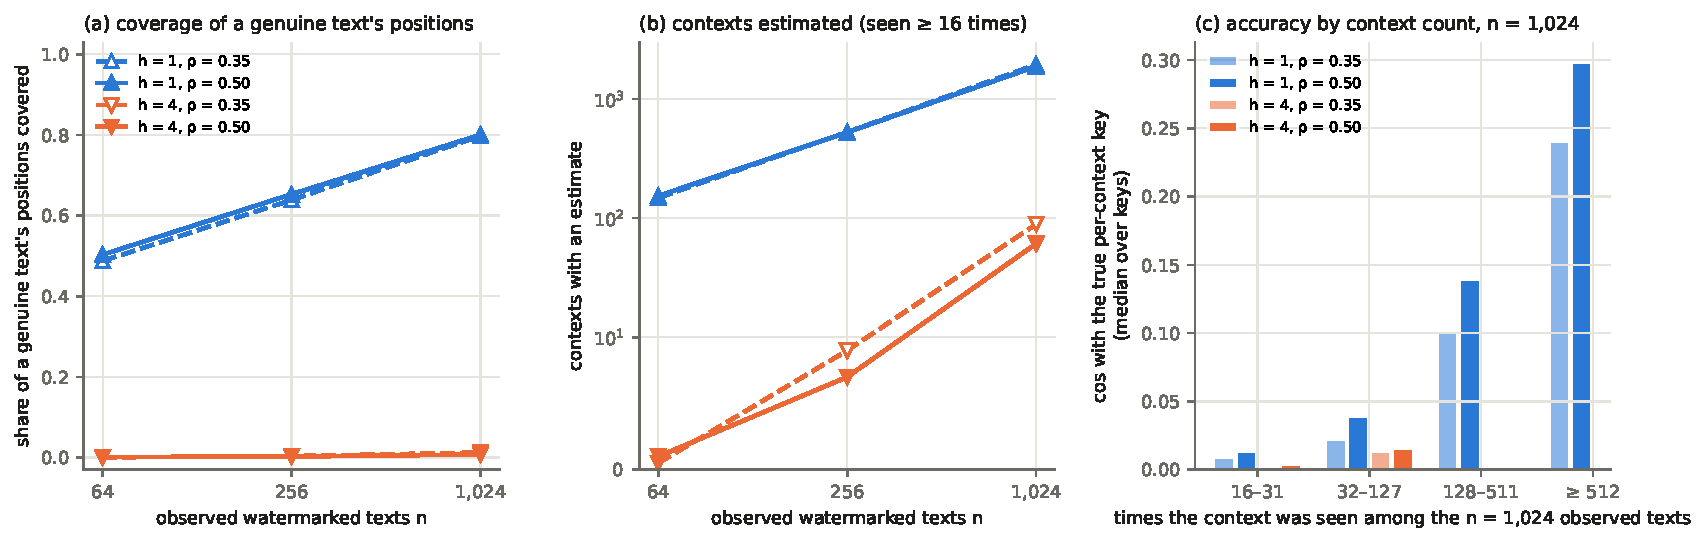
\includegraphics[width=0.8\textwidth,keepaspectratio]{figures/FA4.pdf}
\caption{\textbf{Figure A4.} The per-context attacker on the context-hashed arms: (a) the coverage of a genuine text's positions by estimated contexts and (b) the number of contexts estimated, against the budget n; (c) at n = 1,024, the cosine of the per-context estimates with their true directions by how often the context was seen (medians over 8 keys).}
\end{figure}

Figure A4 shows what this attacker gets from \(n\) texts: the coverage of a genuine text's positions, the number of contexts estimated and the accuracy of the estimates by how often a context was seen (Appendix G.4 reads it).

\hypertarget{the-rotation-attackers}{%
\subsection{The rotation attackers}\label{the-rotation-attackers}}

Against rotation among \(K = 8\) keys the observed texts are a mixture. The \textbf{naive} attacker runs Route A\ensuremath{'} on the mixture; averaging cancels the keys, and its estimate's best cosine with any key was at most 0.000 at \(\rho = 0.35\) and 0.000 at \(\rho = 0.50\) from 1,024 texts (Table A4d). The \textbf{clustering} attacker first clusters the standardised summed gradients by spherical \(k\)-means \citep{dhillon2001spherical} with \(K = 8\) (20 restarts, cosine objective, fixed seed), then runs Route A\ensuremath{'} within each cluster. Its recovery is read as the number of keys for which some cluster's estimate has cosine at least 0.5 with that key: 6 of 8 from 256 texts at \(\rho = 0.35\) and 7 of 8 from 64 texts at \(\rho = 0.50\). The \textbf{pre-registered forgery} used one cluster, the one with the largest standardised mean-gradient profile. At \(\rho = 0.50\) that cluster's estimate had cosine 0.954 with its key at \(n = 64\) and the forgeries were accepted at FA 95.0 {[}90.0, 99.0{]}\%; at \(\rho = 0.35\) the rule picked a small cluster whose estimate had cosine 0.000 with every key at \(n = 256\) (the largest cosine among the clusters was 0.983), so the forgeries failed (FA 2.0 {[}0.0, 5.0{]}\%) although the recovery had succeeded. The pre-registered verdict for rotation at \(\rho = 0.35\) therefore reads ``stealing blocked at n \textless= 1024'' and stands as written; the post-hoc addendum (App. G), labelled and not pre-registered, forged with every cluster's estimate. The lesson we draw for attack evaluations is methodological: pre-register the recovery metric and the forgery as separate readings, and let the attacker forge with every candidate or with its own best-by-objective candidate, never with a single heuristic pick.

{\scriptsize\setlength{\tabcolsep}{1.5pt}\begin{longtable}[]{@{}
  >{\raggedright\arraybackslash}p{(\columnwidth - 18\tabcolsep) * \real{0.0503}}
  >{\raggedright\arraybackslash}p{(\columnwidth - 18\tabcolsep) * \real{0.0653}}
  >{\raggedright\arraybackslash}p{(\columnwidth - 18\tabcolsep) * \real{0.1055}}
  >{\raggedright\arraybackslash}p{(\columnwidth - 18\tabcolsep) * \real{0.1156}}
  >{\raggedright\arraybackslash}p{(\columnwidth - 18\tabcolsep) * \real{0.1055}}
  >{\raggedright\arraybackslash}p{(\columnwidth - 18\tabcolsep) * \real{0.0905}}
  >{\raggedright\arraybackslash}p{(\columnwidth - 18\tabcolsep) * \real{0.1307}}
  >{\raggedright\arraybackslash}p{(\columnwidth - 18\tabcolsep) * \real{0.1156}}
  >{\raggedright\arraybackslash}p{(\columnwidth - 18\tabcolsep) * \real{0.1307}}
  >{\raggedright\arraybackslash}p{(\columnwidth - 18\tabcolsep) * \real{0.0905}}@{}}
\caption{\textbf{Table A4d.} Study 5: the clustering attacker on rotation among 8 keys (spherical k-means with K = 8 on the standardised summed gradients, then Route A\ensuremath{'} per cluster)}\tabularnewline
\toprule\noalign{}
\begin{minipage}[b]{\linewidth}\raggedright
\ensuremath{\rho}
\end{minipage} & \begin{minipage}[b]{\linewidth}\raggedright
n
\end{minipage} & \begin{minipage}[b]{\linewidth}\raggedright
clusters with \ensuremath{\geq} 2 texts
\end{minipage} & \begin{minipage}[b]{\linewidth}\raggedright
keys recovered (best cos \ensuremath{\geq} 0.5)
\end{minipage} & \begin{minipage}[b]{\linewidth}\raggedright
median best cos over clusters
\end{minipage} & \begin{minipage}[b]{\linewidth}\raggedright
largest best cos
\end{minipage} & \begin{minipage}[b]{\linewidth}\raggedright
forging cluster by the pre-registered rule (largest z-profile)
\end{minipage} & \begin{minipage}[b]{\linewidth}\raggedright
naive attacker: best cos with any key
\end{minipage} & \begin{minipage}[b]{\linewidth}\raggedright
forgery FA \%, clustering {[}95\% CI{]}
\end{minipage} & \begin{minipage}[b]{\linewidth}\raggedright
forgery FA \%, naive {[}95\% CI{]}
\end{minipage} \\
\midrule\noalign{}
\endfirsthead
\toprule\noalign{}
\begin{minipage}[b]{\linewidth}\raggedright
\ensuremath{\rho}
\end{minipage} & \begin{minipage}[b]{\linewidth}\raggedright
n
\end{minipage} & \begin{minipage}[b]{\linewidth}\raggedright
clusters with \ensuremath{\geq} 2 texts
\end{minipage} & \begin{minipage}[b]{\linewidth}\raggedright
keys recovered (best cos \ensuremath{\geq} 0.5)
\end{minipage} & \begin{minipage}[b]{\linewidth}\raggedright
median best cos over clusters
\end{minipage} & \begin{minipage}[b]{\linewidth}\raggedright
largest best cos
\end{minipage} & \begin{minipage}[b]{\linewidth}\raggedright
forging cluster by the pre-registered rule (largest z-profile)
\end{minipage} & \begin{minipage}[b]{\linewidth}\raggedright
naive attacker: best cos with any key
\end{minipage} & \begin{minipage}[b]{\linewidth}\raggedright
forgery FA \%, clustering {[}95\% CI{]}
\end{minipage} & \begin{minipage}[b]{\linewidth}\raggedright
forgery FA \%, naive {[}95\% CI{]}
\end{minipage} \\
\midrule\noalign{}
\endhead
\bottomrule\noalign{}
\endlastfoot
0.35 & 64 & 8 & 4 & 0.560 & 0.888 & 6 (size 3; cos 0.308; z-profile 9.09) & 0.000 & 8.0 {[}3.0, 14.0{]} & 0.0 {[}0.0, 0.0{]} \\
0.35 & 256 & 8 & 6 & 0.830 & 0.983 & 1 (size 17; cos 0.000; z-profile 8.21) & 0.000 & 2.0 {[}0.0, 5.0{]} & 1.0 {[}0.0, 3.0{]} \\
0.35 & 1,024 & 8 & 6 & 0.866 & 0.964 & 7 (size 92; cos 0.000; z-profile 9.75) & 0.000 & 0.0 {[}0.0, 0.0{]} & 1.0 {[}0.0, 3.0{]} \\
0.5 & 64 & 8 & 7 & 0.862 & 0.954 & 3 (size 8; cos 0.954; z-profile 6.38) & 0.000 & 95.0 {[}90.0, 99.0{]} & 0.0 {[}0.0, 0.0{]} \\
0.5 & 256 & 8 & 8 & 0.952 & 0.990 & 0 (size 32; cos 0.959; z-profile 6.50) & 0.355 & 95.0 {[}90.0, 99.0{]} & 12.0 {[}6.0, 18.0{]} \\
0.5 & 1,024 & 8 & 8 & 0.950 & 0.991 & 7 (size 128; cos 0.957; z-profile 6.56) & 0.000 & 96.0 {[}92.0, 99.0{]} & 0.0 {[}0.0, 0.0{]} \\
\end{longtable}}

\emph{The pre-registered forgery used the cluster with the largest standardised mean-gradient profile; at \ensuremath{\rho} = 0.35 that rule picked a small cluster whose estimate has cosine near 0 with every key, which is why the forgery acceptance is low although most keys were recovered (the labelled post-hoc addendum, Appendix G, forges with every cluster).}

\hypertarget{the-scrubbing-attackers}{%
\subsection{The scrubbing attackers}\label{the-scrubbing-attackers}}

\textbf{Paraphrase (P-Qwen, P-Phi).} The input is the continuation only, with the fixed paraphrase instruction identified in Section 4, sampled at temperature 0.7 and top-p 0.9 with at most 400 new tokens, in batches sorted by length. The attacker's self-check, computed with its own pool C data, keeps an attempt whose perplexity is at most \(\max(1.25 \times\) the original's, the 95th percentile over the human continuations of its 200 pool C prompts\()\), whose seq-rep-4 is at most \(\max(\)the original's, that 95th percentile\()\), whose length is at least 80\% of the original's and whose embedding cosine with the original exceeds the 95th percentile of its 200 pool C pairs; failing attempts are retried with new seeds up to three times, and if none passes the attacker keeps the attempt failing the fewest conditions.

\textbf{Key-guided word edits (E-true, E-est, E-rand).} The text is the first 256 tokens of the continuation. An edit replaces a whole word (an alphabetic token with a leading space followed by a word boundary) by one of the ten most likely whole-word alternatives at that position among the model's 40 most likely tokens that are at least a third as likely as the current word. The contribution of a candidate word \(y\) at position \(t\) to the detector's statistic is estimated by a symmetric difference, \(c_t(y) = [\log p_+(y) - \log p_-(y)] / 2s\), from two passes with \(\pm s \hat w\) added at the output of the estimate's layer (\(s = 2.0\); float32, because the bfloat16 difference failed a gradient check in the first pilot), with \(\hat w = \hat v \oslash \hat\sigma_{\hat\ell}\), the direction divided by the per-coordinate standard deviation of the gradient over the attacker's 200 reference texts. In each round the positions with the largest gain \(c_t(x_t) - \min_y c_t(y)\), at least two apart from each other and from earlier edits, receive their best candidate; a round edits 5\% of the tokens and the text is saved at 2, 5 and 10\%. E-true uses the true key at layer 14 but not the owner's reference texts (an insider bound); E-est uses Study 1 v0.2's Route A estimate at \(n = \text{1,024}\), its layer and vector as saved; E-rand uses random eligible positions and candidates with the same budgets.

\hypertarget{per-key-tables-and-calibration}{%
\section{Per-key tables and calibration}\label{per-key-tables-and-calibration}}

Every rate in the main text is a median over the 8 study keys with a cluster-bootstrap interval. A median can pass a rule while a few keys fail completely, so this appendix gives the per-unit view behind every median (Tables A6--A9) and the per-key calibration of every test used (Figure A1), together with the key-leakage lens of Study 3 (Figure A2). Per-key heterogeneity is a descriptive reading; the scheme's authors note it for steering directions in general (``Some vectors induce more severe degradations in generation quality, while others are more easily detectable'', p.~7) \citep{ardoin2026selfrecognition}.

\hypertarget{forgery-of-the-probe-per-key}{%
\subsection{Forgery of the probe, per key}\label{forgery-of-the-probe-per-key}}

{\scriptsize\setlength{\tabcolsep}{1.5pt}\begin{longtable}[]{@{}
  >{\raggedright\arraybackslash}p{(\columnwidth - 22\tabcolsep) * \real{0.0625}}
  >{\raggedright\arraybackslash}p{(\columnwidth - 22\tabcolsep) * \real{0.1250}}
  >{\raggedright\arraybackslash}p{(\columnwidth - 22\tabcolsep) * \real{0.0812}}
  >{\raggedright\arraybackslash}p{(\columnwidth - 22\tabcolsep) * \real{0.0812}}
  >{\raggedright\arraybackslash}p{(\columnwidth - 22\tabcolsep) * \real{0.0812}}
  >{\raggedright\arraybackslash}p{(\columnwidth - 22\tabcolsep) * \real{0.0812}}
  >{\raggedright\arraybackslash}p{(\columnwidth - 22\tabcolsep) * \real{0.0812}}
  >{\raggedright\arraybackslash}p{(\columnwidth - 22\tabcolsep) * \real{0.0812}}
  >{\raggedright\arraybackslash}p{(\columnwidth - 22\tabcolsep) * \real{0.0812}}
  >{\raggedright\arraybackslash}p{(\columnwidth - 22\tabcolsep) * \real{0.0812}}
  >{\raggedright\arraybackslash}p{(\columnwidth - 22\tabcolsep) * \real{0.1000}}
  >{\raggedright\arraybackslash}p{(\columnwidth - 22\tabcolsep) * \real{0.0625}}@{}}
\caption{\textbf{Table A6.} Study 1 v0.4: per-key fluent acceptance (FA, \%) by the owner's probe at its 1\% threshold, n = 256 forgeries, with the per-key quality bars}\tabularnewline
\toprule\noalign{}
\begin{minipage}[b]{\linewidth}\raggedright
\ensuremath{\rho}
\end{minipage} & \begin{minipage}[b]{\linewidth}\raggedright
texts
\end{minipage} & \begin{minipage}[b]{\linewidth}\raggedright
1001
\end{minipage} & \begin{minipage}[b]{\linewidth}\raggedright
1002
\end{minipage} & \begin{minipage}[b]{\linewidth}\raggedright
1003
\end{minipage} & \begin{minipage}[b]{\linewidth}\raggedright
1004
\end{minipage} & \begin{minipage}[b]{\linewidth}\raggedright
1005
\end{minipage} & \begin{minipage}[b]{\linewidth}\raggedright
1006
\end{minipage} & \begin{minipage}[b]{\linewidth}\raggedright
1007
\end{minipage} & \begin{minipage}[b]{\linewidth}\raggedright
1008
\end{minipage} & \begin{minipage}[b]{\linewidth}\raggedright
median
\end{minipage} & \begin{minipage}[b]{\linewidth}\raggedright
keys \ensuremath{\geq} the F1 bar (of 8)
\end{minipage} \\
\midrule\noalign{}
\endfirsthead
\toprule\noalign{}
\begin{minipage}[b]{\linewidth}\raggedright
\ensuremath{\rho}
\end{minipage} & \begin{minipage}[b]{\linewidth}\raggedright
texts
\end{minipage} & \begin{minipage}[b]{\linewidth}\raggedright
1001
\end{minipage} & \begin{minipage}[b]{\linewidth}\raggedright
1002
\end{minipage} & \begin{minipage}[b]{\linewidth}\raggedright
1003
\end{minipage} & \begin{minipage}[b]{\linewidth}\raggedright
1004
\end{minipage} & \begin{minipage}[b]{\linewidth}\raggedright
1005
\end{minipage} & \begin{minipage}[b]{\linewidth}\raggedright
1006
\end{minipage} & \begin{minipage}[b]{\linewidth}\raggedright
1007
\end{minipage} & \begin{minipage}[b]{\linewidth}\raggedright
1008
\end{minipage} & \begin{minipage}[b]{\linewidth}\raggedright
median
\end{minipage} & \begin{minipage}[b]{\linewidth}\raggedright
keys \ensuremath{\geq} the F1 bar (of 8)
\end{minipage} \\
\midrule\noalign{}
\endhead
\bottomrule\noalign{}
\endlastfoot
0.35 & genuine (oracle) & 51 & 40 & 16 & 11 & 38 & 16 & 19 & 57 & 28.5 & --- \\
0.35 & random key (generic steering) & 1 & 0 & 3 & 0 & 2 & 0 & 1 & 8 & 1.0 & 0 \\
0.35 & v0.4 Route A, n = 256 & 13 & 6 & 1 & 1 & 13 & 1 & 3 & 6 & 4.5 & 0 \\
0.35 & v0.4 Route B, n = 256 & 15 & 37 & 7 & 2 & 9 & 24 & 31 & 39 & 19.5 & 5 \\
0.35 & perplexity bar (the key's oracle 95th percentile) & 10.3 & 10.5 & 10.0 & 9.9 & 10.8 & 10.4 & 10.7 & 12.2 & 10.5 & --- \\
0.35 & seq-rep-4 bar (the key's oracle 95th percentile) & 0.020 & 0.083 & 0.033 & 0.029 & 0.077 & 0.072 & 0.032 & 0.040 & 0.036 & --- \\
0.50 & genuine (oracle) & 88 & 86 & 64 & 56 & 76 & 78 & 72 & 86 & 77.0 & --- \\
0.50 & random key (generic steering) & 10 & 13 & 10 & 2 & 10 & 12 & 6 & 14 & 10.0 & 0 \\
0.50 & v0.4 Route A, n = 256 & 16 & 20 & 32 & 56 & 36 & 4 & 11 & 76 & 26.0 & 2 \\
0.50 & v0.4 Route B, n = 256 & 25 & 73 & 27 & 2 & 26 & 27 & 8 & 51 & 26.5 & 2 \\
0.50 & perplexity bar (the key's oracle 95th percentile) & 13.9 & 15.7 & 14.2 & 11.9 & 15.3 & 13.1 & 12.9 & 17.4 & 14.1 & --- \\
0.50 & seq-rep-4 bar (the key's oracle 95th percentile) & 0.012 & 0.072 & 0.020 & 0.020 & 0.056 & 0.032 & 0.060 & 0.020 & 0.026 & --- \\
0.70 & genuine (oracle) & 90 & 90 & 95 & 89 & 91 & 90 & 90 & 90 & 90.0 & --- \\
0.70 & random key (generic steering) & 14 & 47 & 49 & 14 & 57 & 53 & 26 & 24 & 36.5 & 4 \\
0.70 & v0.4 Route A, n = 256 & 17 & 75 & 97 & 86 & 77 & 71 & 3 & 5 & 73.0 & 5 \\
0.70 & v0.4 Route B, n = 256 & 11 & 61 & 6 & 3 & 51 & 49 & 2 & 72 & 30.0 & 4 \\
0.70 & perplexity bar (the key's oracle 95th percentile) & 21.7 & 28.4 & 27.9 & 19.1 & 29.5 & 22.0 & 21.1 & 30.6 & 25.0 & --- \\
0.70 & seq-rep-4 bar (the key's oracle 95th percentile) & 0.008 & 0.210 & 0.016 & 0.020 & 0.051 & 0.032 & 0.091 & 0.016 & 0.026 & --- \\
\end{longtable}}

\emph{FA counts a text as accepted by the probe, with perplexity and seq-rep-4 at or below the key's oracle 95th percentiles (the bars in the last two rows of each strength). The F1 bar is half the oracle's median FA; the F1 verdicts (Table 3) use the median over keys with its cluster-bootstrap interval, so a set can be `not practical' or `inconclusive' while some keys exceed the bar.}

At \(\rho = 0.35\), where Route B's forgery is practical (Section 5.2), its fluent acceptance ranges from 2 to 39\% across keys and 5 of 8 keys are at or above the F1 bar of 14.3\%, so the verdict rests on a majority of keys rather than on all of them; Route A's acceptance there stays within 1--13\%. At \(\rho = 0.70\) Route A is bimodal: 5 keys are accepted half the time or more and 3 keys at most a fifth of the time, which is why its interval straddles the bar and the rule reads ``inconclusive'' (Table 3). The last two rows of each strength give the per-key quality bars: the perplexity bar is the key's own genuine 95th percentile and rises from 9.9--12.2 at \(\rho = 0.35\) to 19.1--30.6 at \(0.70\), the point Appendix E returns to.

\hypertarget{the-exact-test-per-key}{%
\subsection{The exact test, per key}\label{the-exact-test-per-key}}

{\scriptsize\setlength{\tabcolsep}{1.5pt}\begin{longtable}[]{@{}
  >{\raggedright\arraybackslash}p{(\columnwidth - 22\tabcolsep) * \real{0.0685}}
  >{\raggedright\arraybackslash}p{(\columnwidth - 22\tabcolsep) * \real{0.1370}}
  >{\raggedright\arraybackslash}p{(\columnwidth - 22\tabcolsep) * \real{0.0685}}
  >{\raggedright\arraybackslash}p{(\columnwidth - 22\tabcolsep) * \real{0.0685}}
  >{\raggedright\arraybackslash}p{(\columnwidth - 22\tabcolsep) * \real{0.0685}}
  >{\raggedright\arraybackslash}p{(\columnwidth - 22\tabcolsep) * \real{0.0685}}
  >{\raggedright\arraybackslash}p{(\columnwidth - 22\tabcolsep) * \real{0.0685}}
  >{\raggedright\arraybackslash}p{(\columnwidth - 22\tabcolsep) * \real{0.0685}}
  >{\raggedright\arraybackslash}p{(\columnwidth - 22\tabcolsep) * \real{0.0685}}
  >{\raggedright\arraybackslash}p{(\columnwidth - 22\tabcolsep) * \real{0.0685}}
  >{\raggedright\arraybackslash}p{(\columnwidth - 22\tabcolsep) * \real{0.1233}}
  >{\raggedright\arraybackslash}p{(\columnwidth - 22\tabcolsep) * \real{0.1233}}@{}}
\caption{\textbf{Table A7a.} Study 3: per-key acceptance by the exact test (S4, p \ensuremath{\leq} 0.01, \%) on the study keys, with the owner's probe's median beside it}\tabularnewline
\toprule\noalign{}
\begin{minipage}[b]{\linewidth}\raggedright
\ensuremath{\rho}
\end{minipage} & \begin{minipage}[b]{\linewidth}\raggedright
texts
\end{minipage} & \begin{minipage}[b]{\linewidth}\raggedright
1001
\end{minipage} & \begin{minipage}[b]{\linewidth}\raggedright
1002
\end{minipage} & \begin{minipage}[b]{\linewidth}\raggedright
1003
\end{minipage} & \begin{minipage}[b]{\linewidth}\raggedright
1004
\end{minipage} & \begin{minipage}[b]{\linewidth}\raggedright
1005
\end{minipage} & \begin{minipage}[b]{\linewidth}\raggedright
1006
\end{minipage} & \begin{minipage}[b]{\linewidth}\raggedright
1007
\end{minipage} & \begin{minipage}[b]{\linewidth}\raggedright
1008
\end{minipage} & \begin{minipage}[b]{\linewidth}\raggedright
median (exact)
\end{minipage} & \begin{minipage}[b]{\linewidth}\raggedright
the probe's median on the same texts
\end{minipage} \\
\midrule\noalign{}
\endfirsthead
\toprule\noalign{}
\begin{minipage}[b]{\linewidth}\raggedright
\ensuremath{\rho}
\end{minipage} & \begin{minipage}[b]{\linewidth}\raggedright
texts
\end{minipage} & \begin{minipage}[b]{\linewidth}\raggedright
1001
\end{minipage} & \begin{minipage}[b]{\linewidth}\raggedright
1002
\end{minipage} & \begin{minipage}[b]{\linewidth}\raggedright
1003
\end{minipage} & \begin{minipage}[b]{\linewidth}\raggedright
1004
\end{minipage} & \begin{minipage}[b]{\linewidth}\raggedright
1005
\end{minipage} & \begin{minipage}[b]{\linewidth}\raggedright
1006
\end{minipage} & \begin{minipage}[b]{\linewidth}\raggedright
1007
\end{minipage} & \begin{minipage}[b]{\linewidth}\raggedright
1008
\end{minipage} & \begin{minipage}[b]{\linewidth}\raggedright
median (exact)
\end{minipage} & \begin{minipage}[b]{\linewidth}\raggedright
the probe's median on the same texts
\end{minipage} \\
\midrule\noalign{}
\endhead
\bottomrule\noalign{}
\endlastfoot
0.25 & genuine (oracle) & 99 & 91 & 98 & 98 & 100 & 93 & 95 & 97 & 97.5 & 8.0 \\
0.25 & random key & 0 & 0 & 0 & 0 & 1 & 1 & 0 & 1 & 0.0 & 1.0 \\
0.25 & v0.2 Route B, n = 1,024 & 0 & 2 & 30 & 3 & 5 & 54 & 5 & 0 & 4.0 & 7.5 \\
0.25 & v0.2 Route A, n = 1,024 & 1 & 7 & 3 & 9 & 13 & 1 & 1 & 0 & 2.0 & 2.0 \\
0.35 & genuine (oracle) & 100 & 95 & 95 & 98 & 96 & 88 & 98 & 96 & 96.0 & 32.0 \\
0.35 & random key & 2 & 0 & 0 & 0 & 0 & 2 & 0 & 0 & 0.0 & 1.5 \\
0.35 & v0.2 Route B, n = 1,024 & 0 & 4 & 45 & 4 & 0 & 48 & 11 & 0 & 4.0 & 45.5 \\
0.35 & v0.4 Route A, n = 256 & 0 & 0 & 6 & 22 & 16 & 13 & 1 & 3 & 4.5 & 4.5 \\
0.35 & v0.4 Route B, n = 256 & 2 & 1 & 8 & 6 & 5 & 50 & 12 & 2 & 5.5 & 22.0 \\
0.50 & genuine (oracle) & 100 & 95 & 99 & 98 & 100 & 99 & 100 & 97 & 99.0 & 86.0 \\
0.50 & random key & 1 & 0 & 0 & 0 & 0 & 2 & 2 & 0 & 0.0 & 13.0 \\
0.50 & v0.2 Route B, n = 1,024 & 0 & 0 & 73 & 86 & 0 & 45 & 6 & 0 & 3.0 & 100.0 \\
0.50 & v0.4 Route A, n = 256 & 1 & 0 & 28 & 97 & 31 & 1 & 1 & 2 & 1.5 & 35.0 \\
0.50 & v0.4 Route B, n = 256 & 0 & 0 & 58 & 4 & 4 & 34 & 10 & 4 & 4.0 & 99.5 \\
0.70 & genuine (oracle) & 100 & 41 & 100 & 100 & 100 & 98 & 100 & 99 & 100.0 & 100.0 \\
0.70 & random key & 0 & 0 & 0 & 0 & 0 & 4 & 1 & 0 & 0.0 & 55.5 \\
0.70 & v0.2 Route B, n = 1,024 & 0 & 0 & 78 & 63 & 3 & 17 & 0 & 0 & 1.5 & 100.0 \\
0.70 & v0.4 Route A, n = 256 & 0 & 0 & 26 & 100 & 2 & 3 & 0 & 1 & 1.5 & 98.5 \\
0.70 & v0.4 Route B, n = 256 & 1 & 0 & 67 & 98 & 2 & 26 & 0 & 1 & 1.5 & 100.0 \\
\end{longtable}}

\emph{Every key is calibrated (Table A7b), so every key counts. The probe's per-key rates were not stored; its median is Study 1's on the same texts.}

{\scriptsize\setlength{\tabcolsep}{1.5pt}\begin{longtable}[]{@{}
  >{\raggedright\arraybackslash}p{(\columnwidth - 22\tabcolsep) * \real{0.1342}}
  >{\raggedright\arraybackslash}p{(\columnwidth - 22\tabcolsep) * \real{0.1342}}
  >{\raggedright\arraybackslash}p{(\columnwidth - 22\tabcolsep) * \real{0.0671}}
  >{\raggedright\arraybackslash}p{(\columnwidth - 22\tabcolsep) * \real{0.0671}}
  >{\raggedright\arraybackslash}p{(\columnwidth - 22\tabcolsep) * \real{0.0671}}
  >{\raggedright\arraybackslash}p{(\columnwidth - 22\tabcolsep) * \real{0.0671}}
  >{\raggedright\arraybackslash}p{(\columnwidth - 22\tabcolsep) * \real{0.0671}}
  >{\raggedright\arraybackslash}p{(\columnwidth - 22\tabcolsep) * \real{0.0671}}
  >{\raggedright\arraybackslash}p{(\columnwidth - 22\tabcolsep) * \real{0.0671}}
  >{\raggedright\arraybackslash}p{(\columnwidth - 22\tabcolsep) * \real{0.0671}}
  >{\raggedright\arraybackslash}p{(\columnwidth - 22\tabcolsep) * \real{0.1074}}
  >{\raggedright\arraybackslash}p{(\columnwidth - 22\tabcolsep) * \real{0.0872}}@{}}
\caption{\textbf{Table A7b.} Study 3: per-key false-positive rates at p \ensuremath{\leq} 0.01 (\%) on 1,000 unwatermarked model texts and 1,000 human continuations per key}\tabularnewline
\toprule\noalign{}
\begin{minipage}[b]{\linewidth}\raggedright
statistic
\end{minipage} & \begin{minipage}[b]{\linewidth}\raggedright
null texts
\end{minipage} & \begin{minipage}[b]{\linewidth}\raggedright
1001
\end{minipage} & \begin{minipage}[b]{\linewidth}\raggedright
1002
\end{minipage} & \begin{minipage}[b]{\linewidth}\raggedright
1003
\end{minipage} & \begin{minipage}[b]{\linewidth}\raggedright
1004
\end{minipage} & \begin{minipage}[b]{\linewidth}\raggedright
1005
\end{minipage} & \begin{minipage}[b]{\linewidth}\raggedright
1006
\end{minipage} & \begin{minipage}[b]{\linewidth}\raggedright
1007
\end{minipage} & \begin{minipage}[b]{\linewidth}\raggedright
1008
\end{minipage} & \begin{minipage}[b]{\linewidth}\raggedright
pooled
\end{minipage} & \begin{minipage}[b]{\linewidth}\raggedright
keys above 3\%
\end{minipage} \\
\midrule\noalign{}
\endfirsthead
\toprule\noalign{}
\begin{minipage}[b]{\linewidth}\raggedright
statistic
\end{minipage} & \begin{minipage}[b]{\linewidth}\raggedright
null texts
\end{minipage} & \begin{minipage}[b]{\linewidth}\raggedright
1001
\end{minipage} & \begin{minipage}[b]{\linewidth}\raggedright
1002
\end{minipage} & \begin{minipage}[b]{\linewidth}\raggedright
1003
\end{minipage} & \begin{minipage}[b]{\linewidth}\raggedright
1004
\end{minipage} & \begin{minipage}[b]{\linewidth}\raggedright
1005
\end{minipage} & \begin{minipage}[b]{\linewidth}\raggedright
1006
\end{minipage} & \begin{minipage}[b]{\linewidth}\raggedright
1007
\end{minipage} & \begin{minipage}[b]{\linewidth}\raggedright
1008
\end{minipage} & \begin{minipage}[b]{\linewidth}\raggedright
pooled
\end{minipage} & \begin{minipage}[b]{\linewidth}\raggedright
keys above 3\%
\end{minipage} \\
\midrule\noalign{}
\endhead
\bottomrule\noalign{}
\endlastfoot
S4 (primary) & unwatermarked model text (pool A), G2 & 0.7 & 0.1 & 0.8 & 0.6 & 1.7 & 1.0 & 1.3 & 0.3 & 0.81 & 0 \\
S4 (primary) & human continuations (pool A), H1 & 0.9 & 0.0 & 0.8 & 1.6 & 0.2 & 0.4 & 1.1 & 0.4 & 0.68 & 0 \\
S3 (secondary) & unwatermarked model text (pool A), G2 & 0.5 & 3.4 & 0.3 & 0.1 & 1.4 & 0.4 & 0.4 & 0.3 & 0.85 & 1 \\
S3 (secondary) & human continuations (pool A), H1 & 1.0 & 1.1 & 1.0 & 0.5 & 0.4 & 0.3 & 0.5 & 0.4 & 0.65 & 0 \\
\end{longtable}}

\emph{G2 excludes a key whose rate on model text exceeds 3\%; S3 (the unstandardised gradient) loses key 1002 by that rule, S4 keeps all eight.}

Every study key is calibrated under S4 (0.1--1.7\% on unwatermarked model text; at most 1.6\% on human continuations), while the unstandardised statistic S3 loses key 1002 at 3.4\% (Table A7b), which is what the power pilot's per-key diagnosis predicted (Appendix B). Two readings were moved here from Section 5.3 for length. The narrowest margin among the ``not practical'' forgery verdicts is Route A at \(\rho = 0.70\) and \(n = 64\), whose upper bound of 42.0\% sits just under the 45.0\% bar. And key 1002 at \(\rho = 0.70\) is attributed for only 41.0\% of its genuine texts where every other key reaches at least 98.0\%; its p-values sit just above the cut-off and its false-positive rate is the lowest of the eight (0.1\%), so its test is conservative in both directions (an exploratory reading from Study 3; unexplained; it changes no verdict, the level's median being 100.0\%). The same key is the weakest under the probe-free union test of rotation (Table A9) and the one that random edits scrub most often (Appendix D.3).

\begin{figure}[htbp]
\centering
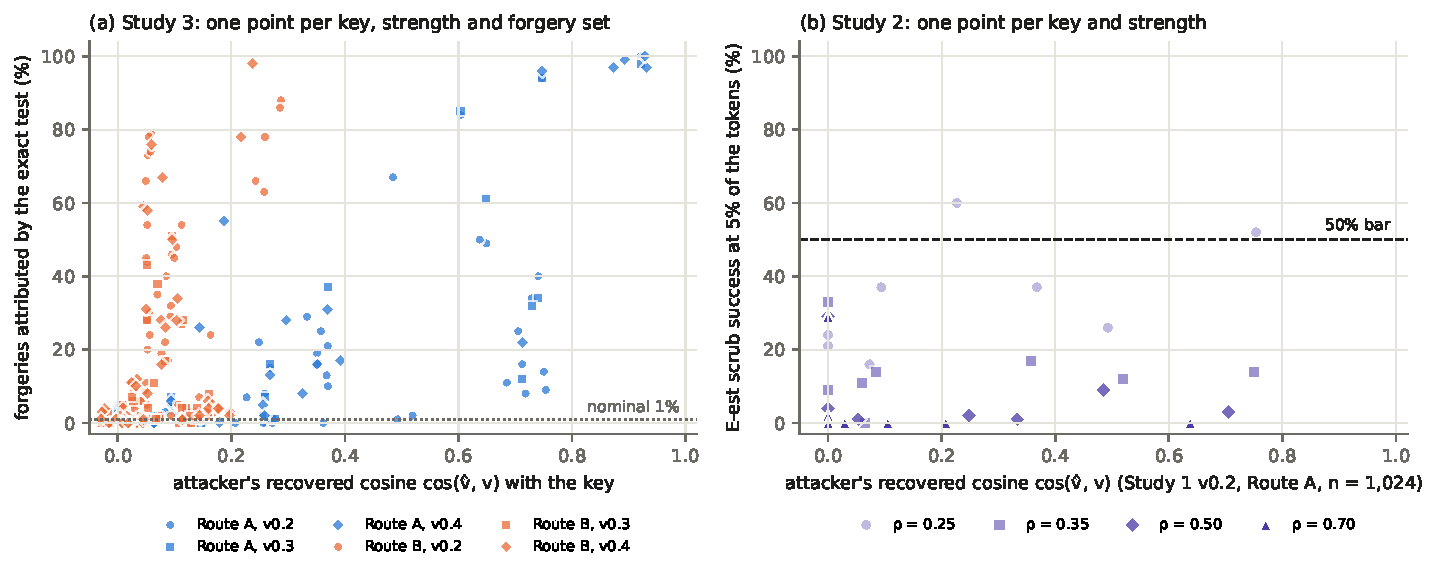
\includegraphics[width=0.8\textwidth,keepaspectratio]{figures/FA2.pdf}
\caption{\textbf{Figure A2.} Key leakage. (a) Study 3: each forgery set's exact-test attribution per key against the attacker's recovered cosine with that key, one point per key, strength and set (Routes A and B; attacker versions v0.2--v0.4). (b) Study 2: E-est's scrub success at 5\% of the tokens against the same cosine, one point per key and strength.}
\end{figure}

The key-leakage lens (Figure A2a; Table A7a) shows where forgeries pass the exact test: in 35 of 384 key--strength--forgery-set cells half or more of the forged texts are attributed, and attribution rises with the attacker's recovered cosine (Spearman 0.68 for Route A and 0.56 for Route B over all cells). For the v0.4 forgeries at \(n = 256\) the cells at or above 50\% are: v0.4 Route B at n = 256, key 1006 at \ensuremath{\rho} = 0.35 (50\%); v0.4 Route A at n = 256, key 1004 at \ensuremath{\rho} = 0.50 (97\%); v0.4 Route B at n = 256, key 1003 at \ensuremath{\rho} = 0.50 (58\%); v0.4 Route A at n = 256, key 1004 at \ensuremath{\rho} = 0.70 (100\%); v0.4 Route B at n = 256, key 1003 at \ensuremath{\rho} = 0.70 (67\%); v0.4 Route B at n = 256, key 1004 at \ensuremath{\rho} = 0.70 (98\%). Route A's forgeries pass where the attack recovered much of the key (key 1004 at \(\rho \geq 0.50\): cosine high, acceptance 97--100\%); some Route B forgeries pass at a cosine near zero (key 1003 and 1006), which we read, as Study 3 did, as the copied footprint reproducing enough of the key's effect on the output distribution for the gradient test to see it (an inference). The protection is therefore only as good as the key's secrecy: with at most 1,024 observed texts this leakage is uncommon for the v0.2--v0.4 attackers and is exactly what Route A\('\) then achieves for every key (Section 5.4).

\hypertarget{scrubbing-per-key}{%
\subsection{Scrubbing, per key}\label{scrubbing-per-key}}

{\scriptsize\setlength{\tabcolsep}{1.5pt}\begin{longtable}[]{@{}
  >{\raggedright\arraybackslash}p{(\columnwidth - 22\tabcolsep) * \real{0.0735}}
  >{\raggedright\arraybackslash}p{(\columnwidth - 22\tabcolsep) * \real{0.1471}}
  >{\raggedright\arraybackslash}p{(\columnwidth - 22\tabcolsep) * \real{0.0735}}
  >{\raggedright\arraybackslash}p{(\columnwidth - 22\tabcolsep) * \real{0.0735}}
  >{\raggedright\arraybackslash}p{(\columnwidth - 22\tabcolsep) * \real{0.0735}}
  >{\raggedright\arraybackslash}p{(\columnwidth - 22\tabcolsep) * \real{0.0735}}
  >{\raggedright\arraybackslash}p{(\columnwidth - 22\tabcolsep) * \real{0.0735}}
  >{\raggedright\arraybackslash}p{(\columnwidth - 22\tabcolsep) * \real{0.0735}}
  >{\raggedright\arraybackslash}p{(\columnwidth - 22\tabcolsep) * \real{0.0735}}
  >{\raggedright\arraybackslash}p{(\columnwidth - 22\tabcolsep) * \real{0.0735}}
  >{\raggedright\arraybackslash}p{(\columnwidth - 22\tabcolsep) * \real{0.1176}}
  >{\raggedright\arraybackslash}p{(\columnwidth - 22\tabcolsep) * \real{0.0735}}@{}}
\caption{\textbf{Table A8.} Study 2: per-key detection before scrubbing and per-key scrub success (\%) by method, 100 texts per key and strength}\tabularnewline
\toprule\noalign{}
\begin{minipage}[b]{\linewidth}\raggedright
\ensuremath{\rho}
\end{minipage} & \begin{minipage}[b]{\linewidth}\raggedright
reading
\end{minipage} & \begin{minipage}[b]{\linewidth}\raggedright
1001
\end{minipage} & \begin{minipage}[b]{\linewidth}\raggedright
1002
\end{minipage} & \begin{minipage}[b]{\linewidth}\raggedright
1003
\end{minipage} & \begin{minipage}[b]{\linewidth}\raggedright
1004
\end{minipage} & \begin{minipage}[b]{\linewidth}\raggedright
1005
\end{minipage} & \begin{minipage}[b]{\linewidth}\raggedright
1006
\end{minipage} & \begin{minipage}[b]{\linewidth}\raggedright
1007
\end{minipage} & \begin{minipage}[b]{\linewidth}\raggedright
1008
\end{minipage} & \begin{minipage}[b]{\linewidth}\raggedright
median
\end{minipage} & \begin{minipage}[b]{\linewidth}\raggedright
keys \ensuremath{\geq} 50\% (of 8)
\end{minipage} \\
\midrule\noalign{}
\endfirsthead
\toprule\noalign{}
\begin{minipage}[b]{\linewidth}\raggedright
\ensuremath{\rho}
\end{minipage} & \begin{minipage}[b]{\linewidth}\raggedright
reading
\end{minipage} & \begin{minipage}[b]{\linewidth}\raggedright
1001
\end{minipage} & \begin{minipage}[b]{\linewidth}\raggedright
1002
\end{minipage} & \begin{minipage}[b]{\linewidth}\raggedright
1003
\end{minipage} & \begin{minipage}[b]{\linewidth}\raggedright
1004
\end{minipage} & \begin{minipage}[b]{\linewidth}\raggedright
1005
\end{minipage} & \begin{minipage}[b]{\linewidth}\raggedright
1006
\end{minipage} & \begin{minipage}[b]{\linewidth}\raggedright
1007
\end{minipage} & \begin{minipage}[b]{\linewidth}\raggedright
1008
\end{minipage} & \begin{minipage}[b]{\linewidth}\raggedright
median
\end{minipage} & \begin{minipage}[b]{\linewidth}\raggedright
keys \ensuremath{\geq} 50\% (of 8)
\end{minipage} \\
\midrule\noalign{}
\endhead
\bottomrule\noalign{}
\endlastfoot
0.25 & detected before scrubbing (unscrubbed originals) & 99 & 91 & 98 & 98 & 100 & 93 & 95 & 97 & 97.5 & 8 \\
0.25 & P-Qwen success & 65 & 71 & 66 & 79 & 58 & 46 & 63 & 55 & 64.0 & 7 \\
0.25 & P-Phi success & 56 & 78 & 56 & 54 & 58 & 44 & 58 & 50 & 56.0 & 7 \\
0.25 & E-true 5\% success & 63 & 90 & 93 & 90 & 78 & 72 & 79 & 79 & 79.0 & 8 \\
0.25 & E-est 5\% success & 16 & 60 & 37 & 52 & 37 & 26 & 21 & 24 & 31.5 & 2 \\
0.25 & E-rand 5\% success & 6 & 28 & 14 & 21 & 19 & 15 & 18 & 24 & 18.5 & 0 \\
0.35 & detected before scrubbing (unscrubbed originals) & 100 & 95 & 95 & 98 & 96 & 88 & 98 & 96 & 96.0 & 8 \\
0.35 & P-Qwen success & 54 & 64 & 52 & 69 & 33 & 34 & 62 & 44 & 53.0 & 5 \\
0.35 & P-Phi success & 38 & 68 & 58 & 46 & 34 & 26 & 46 & 38 & 42.0 & 2 \\
0.35 & E-true 5\% success & 29 & 84 & 64 & 56 & 34 & 35 & 49 & 37 & 43.0 & 3 \\
0.35 & E-est 5\% success & 0 & 33 & 14 & 14 & 17 & 12 & 11 & 9 & 13.0 & 0 \\
0.35 & E-rand 5\% success & 0 & 8 & 7 & 6 & 8 & 9 & 5 & 5 & 6.5 & 0 \\
0.50 & detected before scrubbing (unscrubbed originals) & 100 & 95 & 99 & 98 & 100 & 99 & 100 & 97 & 99.0 & 8 \\
0.50 & P-Qwen success & 37 & 64 & 42 & 44 & 25 & 13 & 45 & 35 & 39.5 & 1 \\
0.50 & P-Phi success & 18 & 64 & 42 & 16 & 16 & 14 & 22 & 22 & 20.0 & 1 \\
0.50 & E-true 5\% success & 16 & 72 & 33 & 10 & 8 & 20 & 17 & 27 & 18.5 & 1 \\
0.50 & E-est 5\% success & 1 & 29 & 9 & 3 & 1 & 2 & 0 & 4 & 2.5 & 0 \\
0.50 & E-rand 5\% success & 1 & 12 & 0 & 3 & 1 & 3 & 0 & 4 & 2.0 & 0 \\
0.70 & detected before scrubbing (unscrubbed originals) & 100 & 41 & 100 & 100 & 100 & 98 & 100 & 99 & 100.0 & 7 \\
0.70 & P-Qwen success & 19 & 53 & 34 & 24 & 14 & 14 & 28 & 29 & 26.0 & 1 \\
0.70 & P-Phi success & 10 & 60 & 16 & 4 & 10 & 2 & 20 & 28 & 13.0 & 1 \\
0.70 & E-true 5\% success & 6 & 43 & 2 & 1 & 3 & 6 & 4 & 5 & 4.5 & 0 \\
0.70 & E-est 5\% success & 0 & 29 & 0 & 0 & 0 & 2 & 0 & 0 & 0.0 & 0 \\
0.70 & E-rand 5\% success & 0 & 35 & 0 & 0 & 1 & 0 & 0 & 0 & 0.0 & 0 \\
\end{longtable}}

\emph{Success: not attributed by the exact test at p \ensuremath{\leq} 0.01 and all four quality conditions pass (perplexity, seq-rep-4, length, embedding similarity against the owner's human-text bars). Every key is calibrated under both paraphrasers (Table A12), so every key counts; the verdicts (Table 5) use the median with its cluster-bootstrap interval.}

P-Qwen's ``effective'' verdict at \(\rho = 0.25\) rests on 7 of 8 keys at or above 50\% and at \(0.35\) on 5; P-Phi at \(0.35\) reaches the bar for 2 keys, the per-key picture behind its inconclusive interval. Key 1002 at \(\rho = 0.70\) was attributed before scrubbing for only 41.0\% of its texts (the same conservative key as above), and random 5\% edits then ``scrub'' it 35.0\% of the time where no other key exceeds 1.0\%, so one key's weak detection, not the edits, produces that cell. Figure A2b plots E-est's success against the accuracy of the v0.2 estimate it used: the estimate's cosine with the key never exceeds 0.75 and the correlation is weak (Spearman 0.13), consistent with the estimate carrying little of the key.

\hypertarget{the-defence-per-key}{%
\subsection{The defence, per key}\label{the-defence-per-key}}

{\scriptsize\setlength{\tabcolsep}{1.5pt}\begin{longtable}[]{@{}
  >{\raggedright\arraybackslash}p{(\columnwidth - 22\tabcolsep) * \real{0.1176}}
  >{\raggedright\arraybackslash}p{(\columnwidth - 22\tabcolsep) * \real{0.0588}}
  >{\raggedright\arraybackslash}p{(\columnwidth - 22\tabcolsep) * \real{0.1176}}
  >{\raggedright\arraybackslash}p{(\columnwidth - 22\tabcolsep) * \real{0.0765}}
  >{\raggedright\arraybackslash}p{(\columnwidth - 22\tabcolsep) * \real{0.0765}}
  >{\raggedright\arraybackslash}p{(\columnwidth - 22\tabcolsep) * \real{0.0765}}
  >{\raggedright\arraybackslash}p{(\columnwidth - 22\tabcolsep) * \real{0.0765}}
  >{\raggedright\arraybackslash}p{(\columnwidth - 22\tabcolsep) * \real{0.0765}}
  >{\raggedright\arraybackslash}p{(\columnwidth - 22\tabcolsep) * \real{0.0765}}
  >{\raggedright\arraybackslash}p{(\columnwidth - 22\tabcolsep) * \real{0.0765}}
  >{\raggedright\arraybackslash}p{(\columnwidth - 22\tabcolsep) * \real{0.0765}}
  >{\raggedright\arraybackslash}p{(\columnwidth - 22\tabcolsep) * \real{0.0941}}@{}}
\caption{\textbf{Table A9.} Study 5: the per-key view behind every median (keys 1001--1008; every key calibrated under every test)}\tabularnewline
\toprule\noalign{}
\begin{minipage}[b]{\linewidth}\raggedright
arm
\end{minipage} & \begin{minipage}[b]{\linewidth}\raggedright
\ensuremath{\rho}
\end{minipage} & \begin{minipage}[b]{\linewidth}\raggedright
reading
\end{minipage} & \begin{minipage}[b]{\linewidth}\raggedright
1001
\end{minipage} & \begin{minipage}[b]{\linewidth}\raggedright
1002
\end{minipage} & \begin{minipage}[b]{\linewidth}\raggedright
1003
\end{minipage} & \begin{minipage}[b]{\linewidth}\raggedright
1004
\end{minipage} & \begin{minipage}[b]{\linewidth}\raggedright
1005
\end{minipage} & \begin{minipage}[b]{\linewidth}\raggedright
1006
\end{minipage} & \begin{minipage}[b]{\linewidth}\raggedright
1007
\end{minipage} & \begin{minipage}[b]{\linewidth}\raggedright
1008
\end{minipage} & \begin{minipage}[b]{\linewidth}\raggedright
median
\end{minipage} \\
\midrule\noalign{}
\endfirsthead
\toprule\noalign{}
\begin{minipage}[b]{\linewidth}\raggedright
arm
\end{minipage} & \begin{minipage}[b]{\linewidth}\raggedright
\ensuremath{\rho}
\end{minipage} & \begin{minipage}[b]{\linewidth}\raggedright
reading
\end{minipage} & \begin{minipage}[b]{\linewidth}\raggedright
1001
\end{minipage} & \begin{minipage}[b]{\linewidth}\raggedright
1002
\end{minipage} & \begin{minipage}[b]{\linewidth}\raggedright
1003
\end{minipage} & \begin{minipage}[b]{\linewidth}\raggedright
1004
\end{minipage} & \begin{minipage}[b]{\linewidth}\raggedright
1005
\end{minipage} & \begin{minipage}[b]{\linewidth}\raggedright
1006
\end{minipage} & \begin{minipage}[b]{\linewidth}\raggedright
1007
\end{minipage} & \begin{minipage}[b]{\linewidth}\raggedright
1008
\end{minipage} & \begin{minipage}[b]{\linewidth}\raggedright
median
\end{minipage} \\
\midrule\noalign{}
\endhead
\bottomrule\noalign{}
\endlastfoot
fixed key (h = 0; S4, Study 3) & --- & FPR on pool A, \% (G2 \ensuremath{\leq} 3) & 0.7 & 0.1 & 0.8 & 0.6 & 1.7 & 1.0 & 1.3 & 0.3 & 0.8 \\
context-hashed, h = 1 & --- & FPR on pool A, \% (G2 \ensuremath{\leq} 3) & 0.9 & 0.8 & 1.0 & 1.0 & 0.3 & 1.4 & 0.4 & 0.8 & 0.8 \\
context-hashed, h = 4 & --- & FPR on pool A, \% (G2 \ensuremath{\leq} 3) & 1.5 & 0.5 & 0.9 & 0.7 & 1.1 & 1.1 & 1.2 & 0.6 & 1.0 \\
fixed key (h = 0) & 0.35 & S4 detection, \% & 100 & 95 & 95 & 98 & 96 & 88 & 98 & 96 & 96 \\
fixed key (h = 0) & 0.35 & genuine FA, \% & 92 & 86 & 86 & 89 & 87 & 83 & 89 & 86 & 86 \\
fixed key (h = 0) & 0.35 & Route A\ensuremath{'} cos(\ensuremath{\hat{v}}, v), known layer, n = 64 & 0.99 & 0.93 & 0.76 & 0.95 & 0.96 & 0.81 & 0.99 & 0.81 & 0.94 \\
fixed key (h = 0) & 0.35 & Route A\ensuremath{'} forgery FA, \%, n = 64 & 92 & 91 & 71 & 94 & 85 & 73 & 92 & 82 & 88 \\
fixed key (h = 0) & 0.35 & Route A\ensuremath{'} cos(\ensuremath{\hat{v}}, v), known layer, n = 1,024 & 0.98 & 0.95 & 0.83 & 0.96 & 0.97 & 0.93 & 0.99 & 0.81 & 0.95 \\
fixed key (h = 0) & 0.35 & Route A\ensuremath{'} forgery FA, \%, n = 1,024 & 79 & 80 & 82 & 89 & 88 & 88 & 89 & 75 & 85 \\
fixed key (h = 0) & 0.35 & Study 2 scrub success (P-Qwen), \% & 54 & 64 & 52 & 69 & 33 & 34 & 62 & 44 & 53 \\
context-hashed, h = 1 & 0.35 & keyed-test detection, \% & 89 & 93 & 93 & 94 & 90 & 93 & 90 & 92 & 92 \\
context-hashed, h = 1 & 0.35 & genuine FA, \% & 79 & 84 & 84 & 85 & 83 & 85 & 81 & 84 & 84 \\
context-hashed, h = 1 & 0.35 & control (random-key) FA, \% & 0 & 0 & 2 & 0 & 1 & 1 & 1 & 1 & 1 \\
context-hashed, h = 1 & 0.35 & per-context forgery FA, \%, n = 1,024 & 3 & 4 & 4 & 2 & 3 & 7 & 9 & 3 & 4 \\
context-hashed, h = 1 & 0.35 & attacker's count-weighted cos, n = 1,024 & 0.156 & 0.169 & 0.171 & 0.196 & 0.159 & 0.246 & 0.168 & 0.214 & 0.170 \\
context-hashed, h = 1 & 0.35 & coverage of a genuine text's positions, n = 1,024 & 0.793 & 0.803 & 0.804 & 0.807 & 0.795 & 0.780 & 0.777 & 0.800 & 0.798 \\
context-hashed, h = 1 & 0.35 & scrub success (P-Qwen), \% & 77 & 73 & 73 & 68 & 78 & 70 & 67 & 78 & 73 \\
context-hashed, h = 1 & 0.35 & d = success \ensuremath{-} the fixed key's, points & +23 & +9 & +21 & -1 & +45 & +36 & +5 & +34 & +22 \\
context-hashed, h = 1 & 0.35 & perplexity ratio to the fixed key (median) & 0.81 & 0.86 & 0.86 & 0.89 & 0.85 & 0.90 & 0.80 & 0.71 & 0.85 \\
context-hashed, h = 4 & 0.35 & keyed-test detection, \% & 91 & 88 & 90 & 87 & 92 & 90 & 90 & 88 & 90 \\
context-hashed, h = 4 & 0.35 & genuine FA, \% & 83 & 78 & 80 & 78 & 85 & 81 & 80 & 79 & 80 \\
context-hashed, h = 4 & 0.35 & control (random-key) FA, \% & 1 & 1 & 0 & 2 & 0 & 0 & 2 & 0 & 0 \\
context-hashed, h = 4 & 0.35 & per-context forgery FA, \%, n = 1,024 & 0 & 0 & 0 & 0 & 0 & 0 & 0 & 0 & 0 \\
context-hashed, h = 4 & 0.35 & attacker's count-weighted cos, n = 1,024 & 0.012 & 0.011 & 0.005 & 0.004 & 0.053 & 0.013 & 0.007 & 0.041 & 0.012 \\
context-hashed, h = 4 & 0.35 & coverage of a genuine text's positions, n = 1,024 & 0.010 & 0.013 & 0.009 & 0.012 & 0.010 & 0.014 & 0.016 & 0.013 & 0.013 \\
context-hashed, h = 4 & 0.35 & scrub success (P-Qwen), \% & 73 & 75 & 69 & 71 & 67 & 78 & 70 & 73 & 72 \\
context-hashed, h = 4 & 0.35 & d = success \ensuremath{-} the fixed key's, points & +19 & +11 & +17 & +2 & +34 & +44 & +8 & +29 & +18 \\
context-hashed, h = 4 & 0.35 & perplexity ratio to the fixed key (median) & 0.81 & 0.84 & 0.86 & 0.90 & 0.83 & 0.90 & 0.81 & 0.67 & 0.83 \\
rotation (K = 8) & 0.35 & union-test detection, \% & 100 & 87 & 87 & 95 & 92 & 87 & 95 & 94 & 93 \\
rotation (K = 8) & 0.35 & single-key detection of the same texts, \% & 100 & 95 & 95 & 98 & 96 & 88 & 98 & 96 & 96 \\
rotation (K = 8) & 0.35 & union-test scrub success on Study 2's paraphrases, \% & 72 & 73 & 68 & 77 & 47 & 50 & 81 & 57 & 70 \\
rotation (K = 8) & 0.35 & d = union-test success \ensuremath{-} the fixed key's, points & +18 & +9 & +16 & +8 & +14 & +16 & +19 & +13 & +15 \\
fixed key (h = 0) & 0.50 & S4 detection, \% & 100 & 95 & 99 & 98 & 100 & 99 & 100 & 97 & 99 \\
fixed key (h = 0) & 0.50 & genuine FA, \% & 90 & 89 & 91 & 91 & 90 & 89 & 90 & 87 & 90 \\
fixed key (h = 0) & 0.50 & Route A\ensuremath{'} cos(\ensuremath{\hat{v}}, v), known layer, n = 64 & 0.99 & 0.90 & 0.90 & 0.96 & 0.97 & 0.95 & 0.99 & 0.81 & 0.95 \\
fixed key (h = 0) & 0.50 & Route A\ensuremath{'} forgery FA, \%, n = 64 & 84 & 92 & 85 & 83 & 89 & 83 & 88 & 86 & 86 \\
fixed key (h = 0) & 0.50 & Route A\ensuremath{'} cos(\ensuremath{\hat{v}}, v), known layer, n = 1,024 & 0.99 & 0.90 & 0.90 & 0.96 & 0.97 & 0.94 & 0.98 & 0.81 & 0.95 \\
fixed key (h = 0) & 0.50 & Route A\ensuremath{'} forgery FA, \%, n = 1,024 & 86 & 89 & 78 & 83 & 93 & 80 & 89 & 91 & 88 \\
fixed key (h = 0) & 0.50 & Study 2 scrub success (P-Qwen), \% & 37 & 64 & 42 & 44 & 25 & 13 & 45 & 35 & 40 \\
context-hashed, h = 1 & 0.50 & keyed-test detection, \% & 97 & 93 & 94 & 96 & 97 & 97 & 95 & 99 & 96 \\
context-hashed, h = 1 & 0.50 & genuine FA, \% & 88 & 87 & 85 & 89 & 88 & 88 & 88 & 89 & 88 \\
context-hashed, h = 1 & 0.50 & control (random-key) FA, \% & 0 & 0 & 0 & 1 & 1 & 1 & 1 & 1 & 1 \\
context-hashed, h = 1 & 0.50 & per-context forgery FA, \%, n = 1,024 & 5 & 9 & 9 & 11 & 6 & 11 & 7 & 9 & 9 \\
context-hashed, h = 1 & 0.50 & attacker's count-weighted cos, n = 1,024 & 0.179 & 0.208 & 0.217 & 0.209 & 0.189 & 0.241 & 0.237 & 0.238 & 0.213 \\
context-hashed, h = 1 & 0.50 & coverage of a genuine text's positions, n = 1,024 & 0.808 & 0.808 & 0.792 & 0.796 & 0.795 & 0.804 & 0.795 & 0.810 & 0.800 \\
context-hashed, h = 1 & 0.50 & scrub success (P-Qwen), \% & 72 & 73 & 69 & 67 & 69 & 68 & 74 & 73 & 70 \\
context-hashed, h = 1 & 0.50 & d = success \ensuremath{-} the fixed key's, points & +35 & +9 & +27 & +23 & +44 & +55 & +29 & +38 & +32 \\
context-hashed, h = 1 & 0.50 & perplexity ratio to the fixed key (median) & 0.69 & 0.71 & 0.80 & 0.82 & 0.71 & 0.80 & 0.73 & 0.61 & 0.72 \\
context-hashed, h = 4 & 0.50 & keyed-test detection, \% & 96 & 95 & 90 & 95 & 96 & 94 & 97 & 97 & 96 \\
context-hashed, h = 4 & 0.50 & genuine FA, \% & 89 & 87 & 83 & 87 & 89 & 86 & 88 & 89 & 88 \\
context-hashed, h = 4 & 0.50 & control (random-key) FA, \% & 0 & 1 & 1 & 0 & 1 & 2 & 0 & 0 & 0 \\
context-hashed, h = 4 & 0.50 & per-context forgery FA, \%, n = 1,024 & 1 & 3 & 2 & 2 & 0 & 0 & 1 & 0 & 1 \\
context-hashed, h = 4 & 0.50 & attacker's count-weighted cos, n = 1,024 & 0.000 & 0.007 & 0.091 & 0.003 & 0.054 & 0.012 & 0.011 & 0.067 & 0.012 \\
context-hashed, h = 4 & 0.50 & coverage of a genuine text's positions, n = 1,024 & 0.007 & 0.009 & 0.009 & 0.008 & 0.007 & 0.007 & 0.007 & 0.008 & 0.008 \\
context-hashed, h = 4 & 0.50 & scrub success (P-Qwen), \% & 69 & 66 & 64 & 67 & 70 & 73 & 78 & 71 & 70 \\
context-hashed, h = 4 & 0.50 & d = success \ensuremath{-} the fixed key's, points & +32 & +2 & +22 & +23 & +45 & +60 & +33 & +36 & +32 \\
context-hashed, h = 4 & 0.50 & perplexity ratio to the fixed key (median) & 0.71 & 0.72 & 0.72 & 0.80 & 0.71 & 0.81 & 0.76 & 0.61 & 0.72 \\
rotation (K = 8) & 0.50 & union-test detection, \% & 99 & 80 & 99 & 97 & 100 & 98 & 100 & 95 & 98 \\
rotation (K = 8) & 0.50 & single-key detection of the same texts, \% & 100 & 95 & 99 & 98 & 100 & 99 & 100 & 97 & 99 \\
rotation (K = 8) & 0.50 & union-test scrub success on Study 2's paraphrases, \% & 46 & 75 & 59 & 62 & 34 & 28 & 63 & 44 & 52 \\
rotation (K = 8) & 0.50 & d = union-test success \ensuremath{-} the fixed key's, points & +9 & +11 & +17 & +18 & +9 & +15 & +18 & +9 & +13 \\
\end{longtable}}

\emph{The fixed key's detection and FA are Study 5's re-scoring of Study 1's texts with S4; its Study 2 scrub success is Study 2's locked value for the same key and strength (asserted equal). d is the keyed arm's scrub success minus the fixed key's, per key; D2 takes its median with a cluster-bootstrap interval. Rotation's texts are the fixed key's, so its quality is unchanged by construction and its paraphrases are Study 2's, scored by the union test.}

For the fixed key, Route A\('\) recovers every key at \(n = 64\) (cosine 0.76--0.99 at \(\rho = 0.35\)) and every key's forgeries at \(n =\) 1,024 exceed the bar (75--89\%; 8 of 8 keys). For the hashed arms no key's forgery acceptance at \(n =\) 1,024 exceeds 11\% (\(h = 1\), \(\rho = 0.50\)). The robustness cost varies: for \(h = 1\) at \(\rho = 0.35\) the per-key difference from the fixed key runs from -1 to +45 points with 5 keys at or above 20 points and 1 key at or below zero; for \(h = 4\) at \(0.35\) only 3 keys reach 20 points, which is the per-key reading behind the inconclusive D2 verdict. Perplexity ratios to the fixed key lie between 0.71 and 0.90 for \(h = 1\) at \(0.35\), below 1 for every key. Rotation's union test detects 80--100\% per key at \(\rho = 0.50\), key 1002 again lowest at 80\%.

\hypertarget{per-key-calibration-before-and-after-paraphrase-and-keying}{%
\subsection{Per-key calibration before and after paraphrase and keying}\label{per-key-calibration-before-and-after-paraphrase-and-keying}}

\begin{figure}[htbp]
\centering
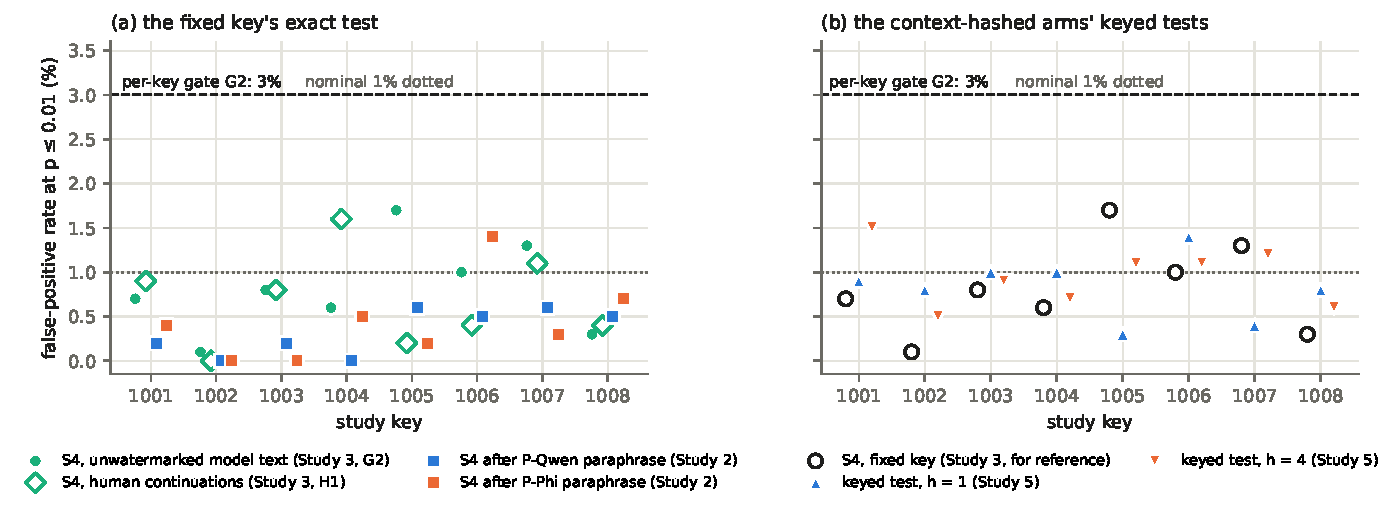
\includegraphics[width=0.8\textwidth,keepaspectratio]{figures/FA1.pdf}
\caption{\textbf{Figure A1.} Per-key false-positive rates at p \ensuremath{\leq} 0.01 on 1,000 null texts per key: (a) the fixed key's exact test on unwatermarked model text and human continuations (Study 3) and after paraphrase by P-Qwen and P-Phi (Study 2); (b) the keyed tests of the context-hashed arms (Study 5) beside the fixed key's. Dotted: the nominal 1\%; dashed: the 3\% per-key gate.}
\end{figure}

Every per-key false-positive rate of the primary test shown in Figure A1 sits under the 3\% gate (the highest, across the fixed key's test on model and human text, after both paraphrasers and under both keyed tests, is 1.7\%); the secondary statistic S3 left key 1002 at 3.4\% (Table A7b), and fresh keys exceed the gate after paraphrase (below), so no verdict excludes a key. The gate is what makes a test that is exact on average over keys usable with one key (Section 3): among 1,000 fresh keys drawn from the same distribution and tested on the paraphrased null texts, 6.5--7.8\% exceed 3\% (maxima 19.5--22.6\%) while the mean stays at 0.94--1.02\% (Table A12b).

\hypertarget{quality-conditions}{%
\section{Quality conditions}\label{quality-conditions}}

\hypertarget{three-fluency-definitions-and-what-each-admits}{%
\subsection{Three fluency definitions and what each admits}\label{three-fluency-definitions-and-what-each-admits}}

{\scriptsize\setlength{\tabcolsep}{1.5pt}\begin{longtable}[]{@{}
  >{\raggedright\arraybackslash}p{(\columnwidth - 18\tabcolsep) * \real{0.0495}}
  >{\raggedright\arraybackslash}p{(\columnwidth - 18\tabcolsep) * \real{0.1040}}
  >{\raggedright\arraybackslash}p{(\columnwidth - 18\tabcolsep) * \real{0.0495}}
  >{\raggedright\arraybackslash}p{(\columnwidth - 18\tabcolsep) * \real{0.1139}}
  >{\raggedright\arraybackslash}p{(\columnwidth - 18\tabcolsep) * \real{0.1040}}
  >{\raggedright\arraybackslash}p{(\columnwidth - 18\tabcolsep) * \real{0.1287}}
  >{\raggedright\arraybackslash}p{(\columnwidth - 18\tabcolsep) * \real{0.1287}}
  >{\raggedright\arraybackslash}p{(\columnwidth - 18\tabcolsep) * \real{0.1287}}
  >{\raggedright\arraybackslash}p{(\columnwidth - 18\tabcolsep) * \real{0.0644}}
  >{\raggedright\arraybackslash}p{(\columnwidth - 18\tabcolsep) * \real{0.1287}}@{}}
\caption{\textbf{Table A10.} Study 1: the same forgeries under three fluency definitions (median over 8 keys, \%); the genuine and random-key texts for reference}\tabularnewline
\toprule\noalign{}
\begin{minipage}[b]{\linewidth}\raggedright
\ensuremath{\rho}
\end{minipage} & \begin{minipage}[b]{\linewidth}\raggedright
route
\end{minipage} & \begin{minipage}[b]{\linewidth}\raggedright
n
\end{minipage} & \begin{minipage}[b]{\linewidth}\raggedright
forgeries
\end{minipage} & \begin{minipage}[b]{\linewidth}\raggedright
accepted by the probe
\end{minipage} & \begin{minipage}[b]{\linewidth}\raggedright
FA, perplexity only (v0.3's rule)
\end{minipage} & \begin{minipage}[b]{\linewidth}\raggedright
FA, perplexity and seq-rep-4 (v0.4's rule)
\end{minipage} & \begin{minipage}[b]{\linewidth}\raggedright
FA, perplexity and word rep-3
\end{minipage} & \begin{minipage}[b]{\linewidth}\raggedright
texts above the seq-rep-4 bar
\end{minipage} & \begin{minipage}[b]{\linewidth}\raggedright
texts under the perplexity bar
\end{minipage} \\
\midrule\noalign{}
\endfirsthead
\toprule\noalign{}
\begin{minipage}[b]{\linewidth}\raggedright
\ensuremath{\rho}
\end{minipage} & \begin{minipage}[b]{\linewidth}\raggedright
route
\end{minipage} & \begin{minipage}[b]{\linewidth}\raggedright
n
\end{minipage} & \begin{minipage}[b]{\linewidth}\raggedright
forgeries
\end{minipage} & \begin{minipage}[b]{\linewidth}\raggedright
accepted by the probe
\end{minipage} & \begin{minipage}[b]{\linewidth}\raggedright
FA, perplexity only (v0.3's rule)
\end{minipage} & \begin{minipage}[b]{\linewidth}\raggedright
FA, perplexity and seq-rep-4 (v0.4's rule)
\end{minipage} & \begin{minipage}[b]{\linewidth}\raggedright
FA, perplexity and word rep-3
\end{minipage} & \begin{minipage}[b]{\linewidth}\raggedright
texts above the seq-rep-4 bar
\end{minipage} & \begin{minipage}[b]{\linewidth}\raggedright
texts under the perplexity bar
\end{minipage} \\
\midrule\noalign{}
\endhead
\bottomrule\noalign{}
\endlastfoot
0.35 & genuine (oracle) & --- & --- & 32.0 & 29.0 & 28.5 & 29.0 & 5.0 & 90.0 \\
0.35 & random key & --- & --- & 1.5 & 1.5 & 1.0 & 1.5 & 7.5 & 89.5 \\
0.35 & Route A & 64 & v0.2 & 11.0 & 7.0 & 7.0 & 7.0 & 5.0 & 89.0 \\
0.35 & Route A & 64 & v0.3 & 9.5 & 4.5 & 4.5 & 4.5 & 6.0 & 91.0 \\
0.35 & Route A & 64 & v0.4 & 4.0 & 4.0 & 4.0 & 4.0 & 5.5 & 91.5 \\
0.35 & Route A & 256 & v0.2 & 3.5 & 3.0 & 3.0 & 3.0 & 6.5 & 90.0 \\
0.35 & Route A & 256 & v0.3 & 7.5 & 7.5 & 6.0 & 7.0 & 10.0 & 87.5 \\
0.35 & Route A & 256 & v0.4 & 4.5 & 4.5 & 4.5 & 4.5 & 10.5 & 87.0 \\
0.35 & Route B & 64 & v0.2 & 42.5 & 3.5 & 0.0 & 1.0 & 17.0 & 45.0 \\
0.35 & Route B & 64 & v0.3 & 20.5 & 16.0 & 8.0 & 7.0 & 16.0 & 65.0 \\
0.35 & Route B & 64 & v0.4 & 10.5 & 9.5 & 9.5 & 9.0 & 8.5 & 82.0 \\
0.35 & Route B & 256 & v0.2 & 56.0 & 11.0 & 9.0 & 9.5 & 18.0 & 39.5 \\
0.35 & Route B & 256 & v0.3 & 19.0 & 15.0 & 13.0 & 12.5 & 9.0 & 70.5 \\
0.35 & Route B & 256 & v0.4 & 22.0 & 20.0 & 19.5 & 19.0 & 6.5 & 85.0 \\
0.50 & genuine (oracle) & --- & --- & 86.0 & 81.0 & 77.0 & 76.0 & 5.0 & 90.0 \\
0.50 & random key & --- & --- & 13.0 & 11.0 & 10.0 & 10.0 & 12.0 & 82.0 \\
0.50 & Route A & 64 & v0.2 & 23.0 & 22.5 & 22.0 & 21.5 & 7.5 & 86.5 \\
0.50 & Route A & 64 & v0.3 & 21.0 & 15.5 & 10.5 & 10.0 & 15.5 & 79.5 \\
0.50 & Route A & 64 & v0.4 & 30.0 & 28.5 & 28.5 & 28.5 & 7.0 & 89.0 \\
0.50 & Route A & 256 & v0.2 & 20.0 & 14.0 & 13.0 & 14.0 & 8.0 & 87.5 \\
0.50 & Route A & 256 & v0.3 & 20.5 & 15.0 & 14.5 & 14.5 & 10.5 & 86.5 \\
0.50 & Route A & 256 & v0.4 & 35.0 & 28.0 & 26.0 & 24.0 & 6.0 & 92.0 \\
0.50 & Route B & 64 & v0.2 & 99.0 & 8.0 & 7.0 & 7.0 & 11.0 & 12.5 \\
0.50 & Route B & 64 & v0.3 & 58.5 & 37.0 & 24.5 & 24.0 & 24.5 & 47.5 \\
0.50 & Route B & 64 & v0.4 & 99.0 & 27.5 & 23.5 & 22.0 & 6.5 & 50.0 \\
0.50 & Route B & 256 & v0.2 & 99.5 & 5.0 & 3.0 & 4.0 & 13.0 & 3.0 \\
0.50 & Route B & 256 & v0.3 & 62.0 & 29.0 & 10.0 & 10.0 & 25.5 & 32.5 \\
0.50 & Route B & 256 & v0.4 & 99.5 & 33.0 & 26.5 & 25.5 & 2.5 & 53.5 \\
0.70 & genuine (oracle) & --- & --- & 100.0 & 95.0 & 90.0 & 90.0 & 5.0 & 90.0 \\
0.70 & random key & --- & --- & 55.5 & 47.5 & 36.5 & 37.5 & 22.5 & 73.0 \\
0.70 & Route A & 64 & v0.2 & 80.5 & 25.0 & 13.0 & 17.0 & 26.0 & 27.0 \\
0.70 & Route A & 64 & v0.3 & 75.5 & 62.5 & 15.0 & 24.0 & 45.0 & 45.0 \\
0.70 & Route A & 64 & v0.4 & 94.5 & 48.0 & 36.5 & 35.5 & 8.5 & 72.5 \\
0.70 & Route A & 256 & v0.2 & 90.5 & 52.5 & 19.5 & 24.0 & 17.0 & 52.5 \\
0.70 & Route A & 256 & v0.3 & 83.0 & 70.5 & 33.0 & 43.0 & 28.5 & 59.5 \\
0.70 & Route A & 256 & v0.4 & 98.5 & 77.5 & 73.0 & 72.0 & 3.5 & 89.0 \\
0.70 & Route B & 64 & v0.2 & 100.0 & 9.0 & 0.5 & 3.0 & 37.5 & 0.5 \\
0.70 & Route B & 64 & v0.3 & 94.0 & 69.0 & 2.5 & 4.5 & 76.0 & 2.5 \\
0.70 & Route B & 64 & v0.4 & 100.0 & 29.5 & 25.5 & 22.5 & 3.0 & 25.5 \\
0.70 & Route B & 256 & v0.2 & 100.0 & 21.5 & 1.0 & 6.0 & 28.5 & 1.0 \\
0.70 & Route B & 256 & v0.3 & 95.0 & 69.0 & 3.0 & 3.5 & 78.0 & 3.0 \\
0.70 & Route B & 256 & v0.4 & 100.0 & 34.0 & 30.0 & 29.0 & 2.0 & 30.0 \\
\end{longtable}}

\emph{v0.2's attacker had no quality check, v0.3's screened its candidate layers by perplexity, v0.4's by perplexity and repetition; every set is re-scored here under v0.4's locked bars (the key's oracle 95th-percentile perplexity and seq-rep-4). The perplexity-only column for the v0.3 forgeries equals v0.3's locked FA (asserted). Word rep-3 is the share of repeated word trigrams, an exploratory alternative to seq-rep-4.}

Study 1's three versions used three quality conditions for a forgery. v0.2 had none: a forgery counted if the probe accepted it. v0.3 added perplexity: a forged text had to be no less fluent than the owner's own watermarked text, measured by continuation perplexity under the unsteered model at or below the key's genuine 95th percentile. v0.4 added a repetition term on both sides, in the attacker's own check and in the evaluation: seq-rep-4 \citep{welleck2020unlikelihood}, the share of a text's token 4-grams that repeat an earlier 4-gram, at or below the key's genuine 95th percentile. Table A10 re-scores every forgery set of the three versions under all three definitions (and under a fourth, exploratory one with word trigrams, which differs from the seq-rep-4 definition by at most 10.0 points in any cell). Two things are visible. v0.2's Route B forgeries at \(\rho \geq 0.50\) are accepted by the probe at least 99.0\% of the time but at most 12.5\% of them pass the perplexity bar: the attacker had chosen layers 0--1 for most keys and the texts were broken multilingual token soup that the probe accepted (v0.2's exploratory reading). And v0.3's perplexity-screened Route B forgeries at \(\rho = 0.70\) reach a perplexity-only acceptance of 69.0\% at \(n = 256\) while 76.0--78.0\% of their texts lie above the repetition bar; under v0.4's definition their acceptance is 3.0\%. Perplexity alone admits loops, because a repeated fragment is highly predictable (Appendix H quotes one), a point the scheme's authors also make (``a highly repetitive, degenerate loop often yields low PPL'', p.~14) \citep{ardoin2026selfrecognition} and that SLAM's four-axis quality evaluation addresses differently \citep{harelcanada2026slam}.

\begin{figure}[htbp]
\centering
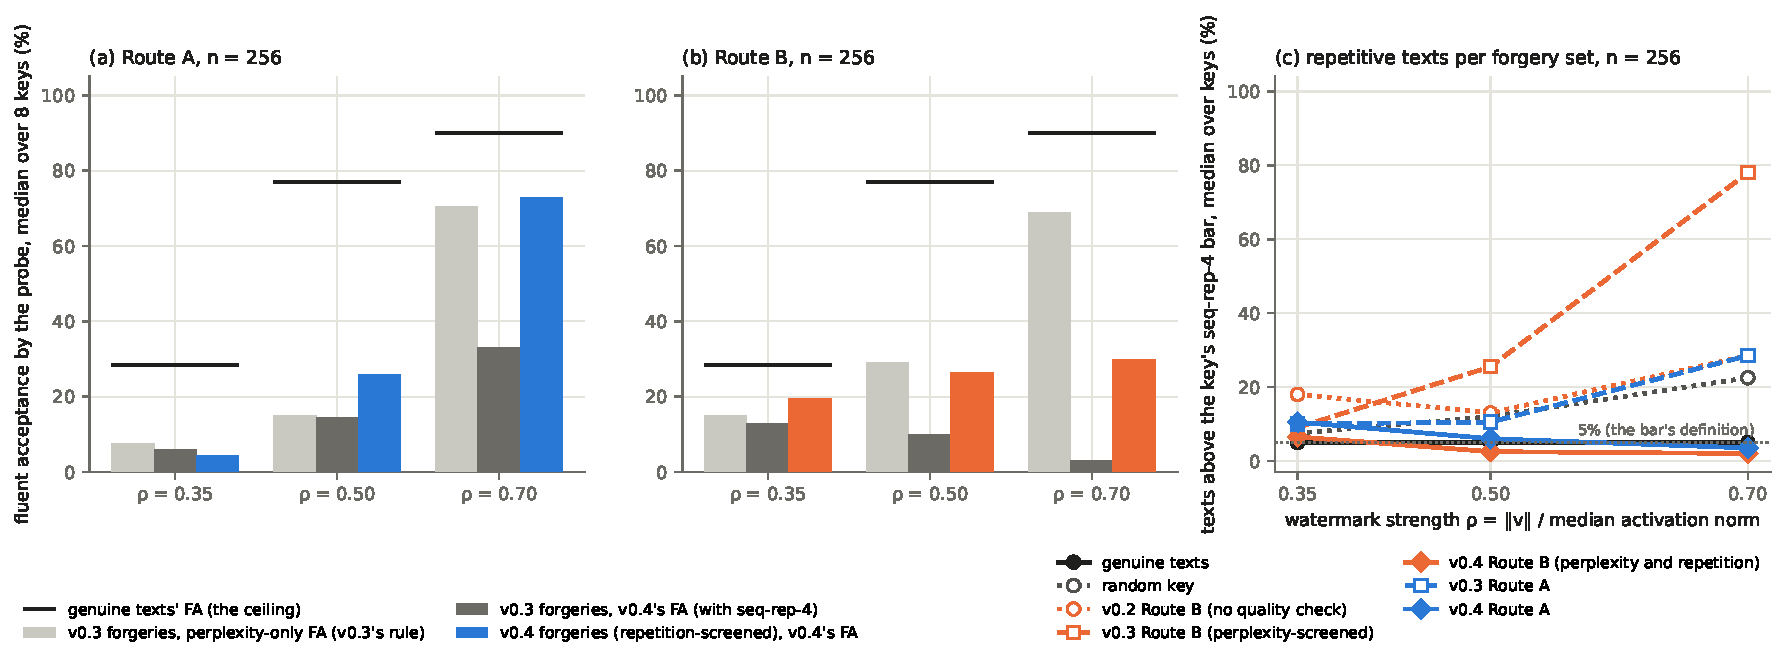
\includegraphics[width=0.8\textwidth,keepaspectratio]{figures/FA5.pdf}
\caption{\textbf{Figure A5.} What the repetition condition changes, n = 256: (a, b) the v0.3 forgeries' fluent acceptance under the perplexity-only rule and under v0.4's rule, and the v0.4 forgeries' acceptance, with the genuine texts' rate as the ceiling; (c) the share of texts above the key's seq-rep-4 bar per forgery set (medians over 8 keys).}
\end{figure}

Figure A5 shows the same movement at \(n = 256\): the repetition term removes most of v0.3's high-strength acceptance (panels a, b), and the share of repetitive texts in v0.4's screened forgeries falls to the genuine texts' level (panel c; the genuine texts' share is 5.0--5.0\% by the bar's construction), where v0.3's Route B reached 78.0\% at \(\rho = 0.70\).

\hypertarget{the-relative-bar-is-lenient-at-the-strongest-watermark}{%
\subsection{The relative bar is lenient at the strongest watermark}\label{the-relative-bar-is-lenient-at-the-strongest-watermark}}

Both of v0.4's bars are relative to the key's genuine watermarked texts, and those texts degrade as the watermark strengthens: the per-key perplexity bar rises from 9.9--12.2 at \(\rho = 0.35\) to 19.1--30.6 at \(0.70\) (Table A6). An exploratory reading after the v0.4 run (prompted by one accepted-and-fluent forgery that is word salad; Appendix H) found the median-perplexity genuine texts at \(\rho = 0.70\) themselves damaged: key 1001's drifts in topic, key 1002's is a repeated web-menu fragment (``Click here to switch between versions: standard-version \ldots{}''), and a higher-perplexity text of key 1001 jumps from politics into an embedded instruction. The word-salad forgery passes both bars (perplexity 27.3 against a bar of 28.4; seq-rep-4 0.016 against 0.210). ``No less fluent than the owner's own watermarked text'' is a fair bar for \emph{forgery}, since an owner cannot reject texts that look like its own output, but at \(\rho = 0.70\) it is a weak bar for \emph{quality}, and the fluent acceptance there should not be read as high-quality forgery (an inference, labelled). At \(\rho = 0.35\) the genuine bar is close to unsteered text and the condition is strict; that is the strength at which Route B's forgery is practical.

Studies 2 and 5 therefore used absolute bars set on the owner's human continuations (the 95th percentile: perplexity 25.4, seq-rep-4 0.048; embedding cosine with the original above 0.825), with two stricter readings reported beside them, the unwatermarked model texts' 95th percentile (perplexity 7.3) and the human median (12.9): under those, P-Qwen's success at \(\rho = 0.35\) falls from 53.0\% to 4.5\% and 16.0\% (Table A12a's companion values), a reminder that ``matched quality'' is a choice of bar.

\hypertarget{study-1-v0.2-in-full}{%
\subsection{Study 1 v0.2 in full}\label{study-1-v0.2-in-full}}

{\footnotesize\begin{longtable}[]{@{}
  >{\raggedright\arraybackslash}p{(\columnwidth - 6\tabcolsep) * \real{0.1282}}
  >{\raggedright\arraybackslash}p{(\columnwidth - 6\tabcolsep) * \real{0.2692}}
  >{\raggedright\arraybackslash}p{(\columnwidth - 6\tabcolsep) * \real{0.2692}}
  >{\raggedright\arraybackslash}p{(\columnwidth - 6\tabcolsep) * \real{0.3333}}@{}}
\caption{\textbf{Table A14a.} Study 1 v0.2: plain acceptance by the owner's probe at its 1\% threshold (median over 8 keys), without any quality condition}\tabularnewline
\toprule\noalign{}
\begin{minipage}[b]{\linewidth}\raggedright
\ensuremath{\rho}
\end{minipage} & \begin{minipage}[b]{\linewidth}\raggedright
texts
\end{minipage} & \begin{minipage}[b]{\linewidth}\raggedright
accepted by the probe (\%) {[}95\% CI{]}
\end{minipage} & \begin{minipage}[b]{\linewidth}\raggedright
median perplexity under the unsteered model
\end{minipage} \\
\midrule\noalign{}
\endfirsthead
\toprule\noalign{}
\begin{minipage}[b]{\linewidth}\raggedright
\ensuremath{\rho}
\end{minipage} & \begin{minipage}[b]{\linewidth}\raggedright
texts
\end{minipage} & \begin{minipage}[b]{\linewidth}\raggedright
accepted by the probe (\%) {[}95\% CI{]}
\end{minipage} & \begin{minipage}[b]{\linewidth}\raggedright
median perplexity under the unsteered model
\end{minipage} \\
\midrule\noalign{}
\endhead
\bottomrule\noalign{}
\endlastfoot
0.25 & genuine (oracle) & 8.0 {[}6.0, 17.0{]} & 6.5 \\
0.25 & random key & 1.0 {[}0.0, 2.0{]} & 6.5 \\
0.25 & Route A, n = 64 & 2.5 {[}0.0, 4.5{]} & 6.1 \\
0.25 & Route A, n = 256 & 1.5 {[}0.0, 3.5{]} & 6.0 \\
0.25 & Route A, n = 1,024 & 2.0 {[}0.0, 3.5{]} & 6.0 \\
0.25 & Route B, n = 64 & 3.0 {[}0.0, 5.5{]} & 6.8 \\
0.25 & Route B, n = 256 & 6.0 {[}2.0, 10.5{]} & 6.8 \\
0.25 & Route B, n = 1,024 & 7.5 {[}2.0, 29.5{]} & 7.2 \\
0.35 & genuine (oracle) & 32.0 {[}17.5, 52.5{]} & 7.7 \\
0.35 & random key & 1.5 {[}0.0, 4.5{]} & 7.7 \\
0.35 & Route A, n = 64 & 11.0 {[}2.5, 22.0{]} & 7.4 \\
0.35 & Route A, n = 256 & 3.5 {[}0.5, 14.5{]} & 7.0 \\
0.35 & Route A, n = 1,024 & 4.5 {[}1.0, 16.0{]} & 6.9 \\
0.35 & Route B, n = 64 & 42.5 {[}5.0, 68.0{]} & 10.4 \\
0.35 & Route B, n = 256 & 56.0 {[}14.0, 80.5{]} & 10.5 \\
0.35 & Route B, n = 1,024 & 45.5 {[}8.0, 87.5{]} & 10.3 \\
0.50 & genuine (oracle) & 86.0 {[}73.5, 94.5{]} & 10.5 \\
0.50 & random key & 13.0 {[}8.0, 18.5{]} & 10.5 \\
0.50 & Route A, n = 64 & 23.0 {[}6.5, 71.5{]} & 8.8 \\
0.50 & Route A, n = 256 & 20.0 {[}5.5, 35.5{]} & 8.8 \\
0.50 & Route A, n = 1,024 & 20.5 {[}8.5, 69.3{]} & 9.5 \\
0.50 & Route B, n = 64 & 99.0 {[}90.5, 100.0{]} & 17.2 \\
0.50 & Route B, n = 256 & 99.5 {[}96.0, 100.0{]} & 17.8 \\
0.50 & Route B, n = 1,024 & 100.0 {[}95.5, 100.0{]} & 18.2 \\
0.70 & genuine (oracle) & 100.0 {[}100.0, 100.0{]} & 16.8 \\
0.70 & random key & 55.5 {[}34.0, 83.0{]} & 16.5 \\
0.70 & Route A, n = 64 & 80.5 {[}24.0, 100.0{]} & 10.0 \\
0.70 & Route A, n = 256 & 90.5 {[}76.5, 100.0{]} & 13.7 \\
0.70 & Route A, n = 1,024 & 89.0 {[}69.5, 100.0{]} & 11.7 \\
0.70 & Route B, n = 64 & 100.0 {[}99.0, 100.0{]} & 30.6 \\
0.70 & Route B, n = 256 & 100.0 {[}100.0, 100.0{]} & 30.5 \\
0.70 & Route B, n = 1,024 & 100.0 {[}100.0, 100.0{]} & 31.1 \\
\end{longtable}}

\emph{Calibration: pooled false-positive rate 1.43\% on unwatermarked model text (G1), 3.6\% on human continuations (exploratory). Perplexity is the median over the set's texts under the unsteered model; a low value can also mean repetitive text (Appendix E).}

{\footnotesize\begin{longtable}[]{@{}
  >{\raggedright\arraybackslash}p{(\columnwidth - 12\tabcolsep) * \real{0.0581}}
  >{\raggedright\arraybackslash}p{(\columnwidth - 12\tabcolsep) * \real{0.1221}}
  >{\raggedright\arraybackslash}p{(\columnwidth - 12\tabcolsep) * \real{0.1512}}
  >{\raggedright\arraybackslash}p{(\columnwidth - 12\tabcolsep) * \real{0.1977}}
  >{\raggedright\arraybackslash}p{(\columnwidth - 12\tabcolsep) * \real{0.1977}}
  >{\raggedright\arraybackslash}p{(\columnwidth - 12\tabcolsep) * \real{0.1977}}
  >{\raggedright\arraybackslash}p{(\columnwidth - 12\tabcolsep) * \real{0.0756}}@{}}
\caption{\textbf{Table A14b.} Study 1 v0.2: key recovery against the budget n (medians over 8 keys) and the pre-registered verdicts}\tabularnewline
\toprule\noalign{}
\begin{minipage}[b]{\linewidth}\raggedright
\ensuremath{\rho}
\end{minipage} & \begin{minipage}[b]{\linewidth}\raggedright
n
\end{minipage} & \begin{minipage}[b]{\linewidth}\raggedright
Route A: median cos(\ensuremath{\hat{v}}, v)
\end{minipage} & \begin{minipage}[b]{\linewidth}\raggedright
Route A: layer 14 found (keys of 8)
\end{minipage} & \begin{minipage}[b]{\linewidth}\raggedright
Route A: median support hit (of k = 4)
\end{minipage} & \begin{minipage}[b]{\linewidth}\raggedright
Route B: median cos(\ensuremath{\hat{v}}, v)
\end{minipage} & \begin{minipage}[b]{\linewidth}\raggedright
Route B: layer 14 found (keys of 8)
\end{minipage} \\
\midrule\noalign{}
\endfirsthead
\toprule\noalign{}
\begin{minipage}[b]{\linewidth}\raggedright
\ensuremath{\rho}
\end{minipage} & \begin{minipage}[b]{\linewidth}\raggedright
n
\end{minipage} & \begin{minipage}[b]{\linewidth}\raggedright
Route A: median cos(\ensuremath{\hat{v}}, v)
\end{minipage} & \begin{minipage}[b]{\linewidth}\raggedright
Route A: layer 14 found (keys of 8)
\end{minipage} & \begin{minipage}[b]{\linewidth}\raggedright
Route A: median support hit (of k = 4)
\end{minipage} & \begin{minipage}[b]{\linewidth}\raggedright
Route B: median cos(\ensuremath{\hat{v}}, v)
\end{minipage} & \begin{minipage}[b]{\linewidth}\raggedright
Route B: layer 14 found (keys of 8)
\end{minipage} \\
\midrule\noalign{}
\endhead
\bottomrule\noalign{}
\endlastfoot
0.25 & 1 & 0.000 & 0 & 0.00 & 0.006 & 0 \\
0.25 & 4 & 0.000 & 0 & 0.00 & 0.021 & 0 \\
0.25 & 16 & 0.000 & 0 & 0.00 & 0.023 & 0 \\
0.25 & 64 & 0.000 & 0 & 0.00 & 0.042 & 3 \\
0.25 & 256 & 0.124 & 1 & 0.25 & 0.045 & 2 \\
0.25 & 1,024 & 0.160 & 2 & 0.25 & 0.054 & 2 \\
0.25 & verdicts & L1 working watermark: no & R1: (descriptive) fails at this budget & R2 A: (descriptive) inconclusive & R2 B: (descriptive) inconclusive & R3: no \\
0.35 & 1 & 0.000 & 1 & 0.00 & 0.001 & 0 \\
0.35 & 4 & 0.000 & 1 & 0.00 & 0.018 & 0 \\
0.35 & 16 & 0.000 & 0 & 0.00 & 0.028 & 2 \\
0.35 & 64 & 0.105 & 1 & 0.25 & 0.036 & 2 \\
0.35 & 256 & 0.079 & 2 & 0.25 & 0.050 & 2 \\
0.35 & 1,024 & 0.074 & 2 & 0.25 & 0.050 & 2 \\
0.35 & verdicts & L1 working watermark: yes & R1: fails at this budget & R2 A: inconclusive & R2 B: practical (n=64) & R3: no \\
0.50 & 1 & 0.000 & 0 & 0.00 & 0.013 & 0 \\
0.50 & 4 & 0.000 & 2 & 0.00 & 0.020 & 0 \\
0.50 & 16 & 0.032 & 3 & 0.12 & 0.043 & 2 \\
0.50 & 64 & 0.000 & 1 & 0.00 & 0.037 & 2 \\
0.50 & 256 & 0.000 & 2 & 0.00 & 0.046 & 2 \\
0.50 & 1,024 & 0.151 & 1 & 0.25 & 0.047 & 2 \\
0.50 & verdicts & L1 working watermark: yes & R1: fails at this budget & R2 A: not practical & R2 B: practical (n=64) & R3: no \\
0.70 & 1 & 0.000 & 0 & 0.00 & 0.027 & 0 \\
0.70 & 4 & 0.000 & 0 & 0.00 & 0.032 & 1 \\
0.70 & 16 & 0.000 & 0 & 0.00 & 0.048 & 2 \\
0.70 & 64 & 0.000 & 1 & 0.00 & 0.046 & 1 \\
0.70 & 256 & 0.000 & 2 & 0.00 & 0.044 & 1 \\
0.70 & 1,024 & 0.015 & 2 & 0.12 & 0.043 & 1 \\
0.70 & verdicts & L1 working watermark: yes & R1: fails at this budget & R2 A: not practical & R2 B: practical (n=64) & R3: yes \\
\end{longtable}}

\emph{Route A estimates the key as the mean activation difference between observed and unwatermarked texts at the attacker's chosen layer; Route B fits a probe and takes its direction. R1 asks, at some n, for a median cosine \ensuremath{\geq} 0.9 with the layer found for at least 7 of 8 keys (the smallest such n is n}), and reads `partial' if the median cosine at n = 1,024 is in {[}0.5, 0.9); it fails at every strength.*

Table A14 gives v0.2's plain acceptance by the probe for every forgery set and budget with the texts' median perplexity, and its key recovery against \(n\): Route A's median cosine with the key never exceeds 0.160 and its layer search finds layer 14 for at most 3 of 8 keys at any budget, Route B's cosine stays at most 0.054, and the pre-registered rules read L1 (a working watermark) no at \(\rho = 0.25\) and yes above it, R1 (recovery) failing at every strength, and R2 (forgery) practical for Route B at \(n = 64\) from \(\rho = 0.35\). The probe's false-positive rate on human continuations in that study was 3.6\% against its nominal 1\% on model text (exploratory), the first sign that it responds to off-distribution text rather than to the key.

{\footnotesize\begin{longtable}[]{@{}
  >{\raggedright\arraybackslash}p{(\columnwidth - 8\tabcolsep) * \real{0.0840}}
  >{\raggedright\arraybackslash}p{(\columnwidth - 8\tabcolsep) * \real{0.3361}}
  >{\raggedright\arraybackslash}p{(\columnwidth - 8\tabcolsep) * \real{0.1513}}
  >{\raggedright\arraybackslash}p{(\columnwidth - 8\tabcolsep) * \real{0.1345}}
  >{\raggedright\arraybackslash}p{(\columnwidth - 8\tabcolsep) * \real{0.2941}}@{}}
\caption{\textbf{Table A15.} Key recovery by the activation-mean estimator (Study 1 v0.2, rule R1) and what the repetition condition changed for v0.3's Route B forgeries at \ensuremath{\rho} = 0.70 (re-scored in v0.4)}\tabularnewline
\toprule\noalign{}
\begin{minipage}[b]{\linewidth}\raggedright
\ensuremath{\rho}
\end{minipage} & \begin{minipage}[b]{\linewidth}\raggedright
quantity
\end{minipage} & \begin{minipage}[b]{\linewidth}\raggedright
median cos(\ensuremath{\hat{v}}, v) at n = 64 / 256 / 1,024 (or FA, \%)
\end{minipage} & \begin{minipage}[b]{\linewidth}\raggedright
layer = 14 (keys of 8) at n = 64 / 256 / 1,024 (or share, \%)
\end{minipage} & \begin{minipage}[b]{\linewidth}\raggedright
verdict
\end{minipage} \\
\midrule\noalign{}
\endfirsthead
\toprule\noalign{}
\begin{minipage}[b]{\linewidth}\raggedright
\ensuremath{\rho}
\end{minipage} & \begin{minipage}[b]{\linewidth}\raggedright
quantity
\end{minipage} & \begin{minipage}[b]{\linewidth}\raggedright
median cos(\ensuremath{\hat{v}}, v) at n = 64 / 256 / 1,024 (or FA, \%)
\end{minipage} & \begin{minipage}[b]{\linewidth}\raggedright
layer = 14 (keys of 8) at n = 64 / 256 / 1,024 (or share, \%)
\end{minipage} & \begin{minipage}[b]{\linewidth}\raggedright
verdict
\end{minipage} \\
\midrule\noalign{}
\endhead
\bottomrule\noalign{}
\endlastfoot
0.25 & Route A key recovery (v0.2) & 0.00 / 0.12 / 0.16 & 0 / 1 / 2 & fails at this budget \\
0.35 & Route A key recovery (v0.2) & 0.10 / 0.08 / 0.07 & 1 / 2 / 2 & fails at this budget \\
0.5 & Route A key recovery (v0.2) & 0.00 / 0.00 / 0.15 & 1 / 2 / 1 & fails at this budget \\
0.7 & Route A key recovery (v0.2) & 0.00 / 0.00 / 0.01 & 1 / 2 / 2 & fails at this budget \\
0.7 & v0.3 Route B forgeries, n = 64: perplexity-only FA \ensuremath{\rightarrow} FA with the repetition term; share above the repetition bar & 69.0 \ensuremath{\rightarrow} 2.5 & 76.0 & v0.3 F1 Route B at 0.70: inconclusive; F3 at 0.70 under v0.3's rule: yes \\
0.7 & v0.3 Route B forgeries, n = 256: perplexity-only FA \ensuremath{\rightarrow} FA with the repetition term; share above the repetition bar & 69.0 \ensuremath{\rightarrow} 3.0 & 78.0 & v0.3 F1 Route B at 0.70: inconclusive; F3 at 0.70 under v0.3's rule: yes \\
\end{longtable}}

\emph{R1 asks for a median cosine of at least 0.9 with the layer found for at least 7 of 8 keys at some n \ensuremath{\leq} 1,024. `Share above the repetition bar' is the median over keys of the share of a condition's texts whose seq-rep-4 exceeds the key-level oracle's 95th percentile.}

\hypertarget{scrubbing-secondaries}{%
\section{Scrubbing secondaries}\label{scrubbing-secondaries}}

\hypertarget{the-edit-curve}{%
\subsection{The edit curve}\label{the-edit-curve}}

{\scriptsize\setlength{\tabcolsep}{1.5pt}\begin{longtable}[]{@{}
  >{\raggedright\arraybackslash}p{(\columnwidth - 22\tabcolsep) * \real{0.0543}}
  >{\raggedright\arraybackslash}p{(\columnwidth - 22\tabcolsep) * \real{0.1087}}
  >{\raggedright\arraybackslash}p{(\columnwidth - 22\tabcolsep) * \real{0.1087}}
  >{\raggedright\arraybackslash}p{(\columnwidth - 22\tabcolsep) * \real{0.0978}}
  >{\raggedright\arraybackslash}p{(\columnwidth - 22\tabcolsep) * \real{0.0978}}
  >{\raggedright\arraybackslash}p{(\columnwidth - 22\tabcolsep) * \real{0.0978}}
  >{\raggedright\arraybackslash}p{(\columnwidth - 22\tabcolsep) * \real{0.1087}}
  >{\raggedright\arraybackslash}p{(\columnwidth - 22\tabcolsep) * \real{0.0543}}
  >{\raggedright\arraybackslash}p{(\columnwidth - 22\tabcolsep) * \real{0.0543}}
  >{\raggedright\arraybackslash}p{(\columnwidth - 22\tabcolsep) * \real{0.1087}}
  >{\raggedright\arraybackslash}p{(\columnwidth - 22\tabcolsep) * \real{0.0543}}
  >{\raggedright\arraybackslash}p{(\columnwidth - 22\tabcolsep) * \real{0.0543}}@{}}
\caption{\textbf{Table A11.} Study 2: the edit curve (median over 8 keys, \%); the pre-registered judgement point is 5\%}\tabularnewline
\toprule\noalign{}
\begin{minipage}[b]{\linewidth}\raggedright
\ensuremath{\rho}
\end{minipage} & \begin{minipage}[b]{\linewidth}\raggedright
arm
\end{minipage} & \begin{minipage}[b]{\linewidth}\raggedright
success at 0\% (the originals' miss rate)
\end{minipage} & \begin{minipage}[b]{\linewidth}\raggedright
success 2\%
\end{minipage} & \begin{minipage}[b]{\linewidth}\raggedright
success 5\%
\end{minipage} & \begin{minipage}[b]{\linewidth}\raggedright
success 10\%
\end{minipage} & \begin{minipage}[b]{\linewidth}\raggedright
detected after 2\%
\end{minipage} & \begin{minipage}[b]{\linewidth}\raggedright
5\%
\end{minipage} & \begin{minipage}[b]{\linewidth}\raggedright
10\%
\end{minipage} & \begin{minipage}[b]{\linewidth}\raggedright
all four quality conditions pass, 2\%
\end{minipage} & \begin{minipage}[b]{\linewidth}\raggedright
5\%
\end{minipage} & \begin{minipage}[b]{\linewidth}\raggedright
10\%
\end{minipage} \\
\midrule\noalign{}
\endfirsthead
\toprule\noalign{}
\begin{minipage}[b]{\linewidth}\raggedright
\ensuremath{\rho}
\end{minipage} & \begin{minipage}[b]{\linewidth}\raggedright
arm
\end{minipage} & \begin{minipage}[b]{\linewidth}\raggedright
success at 0\% (the originals' miss rate)
\end{minipage} & \begin{minipage}[b]{\linewidth}\raggedright
success 2\%
\end{minipage} & \begin{minipage}[b]{\linewidth}\raggedright
success 5\%
\end{minipage} & \begin{minipage}[b]{\linewidth}\raggedright
success 10\%
\end{minipage} & \begin{minipage}[b]{\linewidth}\raggedright
detected after 2\%
\end{minipage} & \begin{minipage}[b]{\linewidth}\raggedright
5\%
\end{minipage} & \begin{minipage}[b]{\linewidth}\raggedright
10\%
\end{minipage} & \begin{minipage}[b]{\linewidth}\raggedright
all four quality conditions pass, 2\%
\end{minipage} & \begin{minipage}[b]{\linewidth}\raggedright
5\%
\end{minipage} & \begin{minipage}[b]{\linewidth}\raggedright
10\%
\end{minipage} \\
\midrule\noalign{}
\endhead
\bottomrule\noalign{}
\endlastfoot
0.25 & E-true (true key) & 2.5 & 35.5 & 79.0 & 81.0 & 64.0 & 21.0 & 0.5 & 100.0 & 99.0 & 81.5 \\
0.25 & E-est (Route A estimate) & 2.5 & 17.5 & 31.5 & 50.5 & 82.0 & 68.0 & 39.5 & 100.0 & 99.0 & 81.5 \\
0.25 & E-rand (random) & 2.5 & 8.0 & 18.5 & 31.0 & 92.0 & 81.5 & 62.5 & 100.0 & 99.5 & 89.5 \\
0.35 & E-true (true key) & 4.0 & 13.5 & 43.0 & 62.0 & 86.0 & 55.5 & 7.0 & 99.5 & 98.0 & 64.0 \\
0.35 & E-est (Route A estimate) & 4.0 & 9.5 & 13.0 & 24.0 & 90.5 & 85.5 & 65.5 & 99.5 & 98.5 & 66.0 \\
0.35 & E-rand (random) & 4.0 & 5.0 & 6.5 & 10.5 & 95.0 & 93.0 & 85.0 & 100.0 & 99.0 & 76.0 \\
0.50 & E-true (true key) & 1.0 & 3.0 & 18.5 & 28.0 & 96.5 & 80.5 & 19.5 & 99.0 & 95.5 & 29.5 \\
0.50 & E-est (Route A estimate) & 1.0 & 3.0 & 2.5 & 6.0 & 97.0 & 97.0 & 88.0 & 100.0 & 93.5 & 32.0 \\
0.50 & E-rand (random) & 1.0 & 1.5 & 2.0 & 3.0 & 98.5 & 98.0 & 96.0 & 99.5 & 96.0 & 42.5 \\
0.70 & E-true (true key) & 0.0 & 1.0 & 4.5 & 3.0 & 98.5 & 89.5 & 40.0 & 89.5 & 41.5 & 3.5 \\
0.70 & E-est (Route A estimate) & 0.0 & 0.5 & 0.0 & 1.0 & 99.0 & 99.0 & 94.5 & 88.5 & 38.5 & 3.5 \\
0.70 & E-rand (random) & 0.0 & 0.5 & 0.0 & 0.0 & 99.5 & 98.5 & 97.5 & 91.5 & 39.0 & 3.5 \\
\end{longtable}}

\emph{Detection: attributed by the exact test at p \ensuremath{\leq} 0.01. Quality: perplexity, seq-rep-4, length and embedding similarity against the owner's human-text bars; at 10\% the perplexity condition fails for most texts at \ensuremath{\rho} \ensuremath{\geq} 0.50, which is why removal of the evidence there does not count as success.}

\begin{figure}[htbp]
\centering
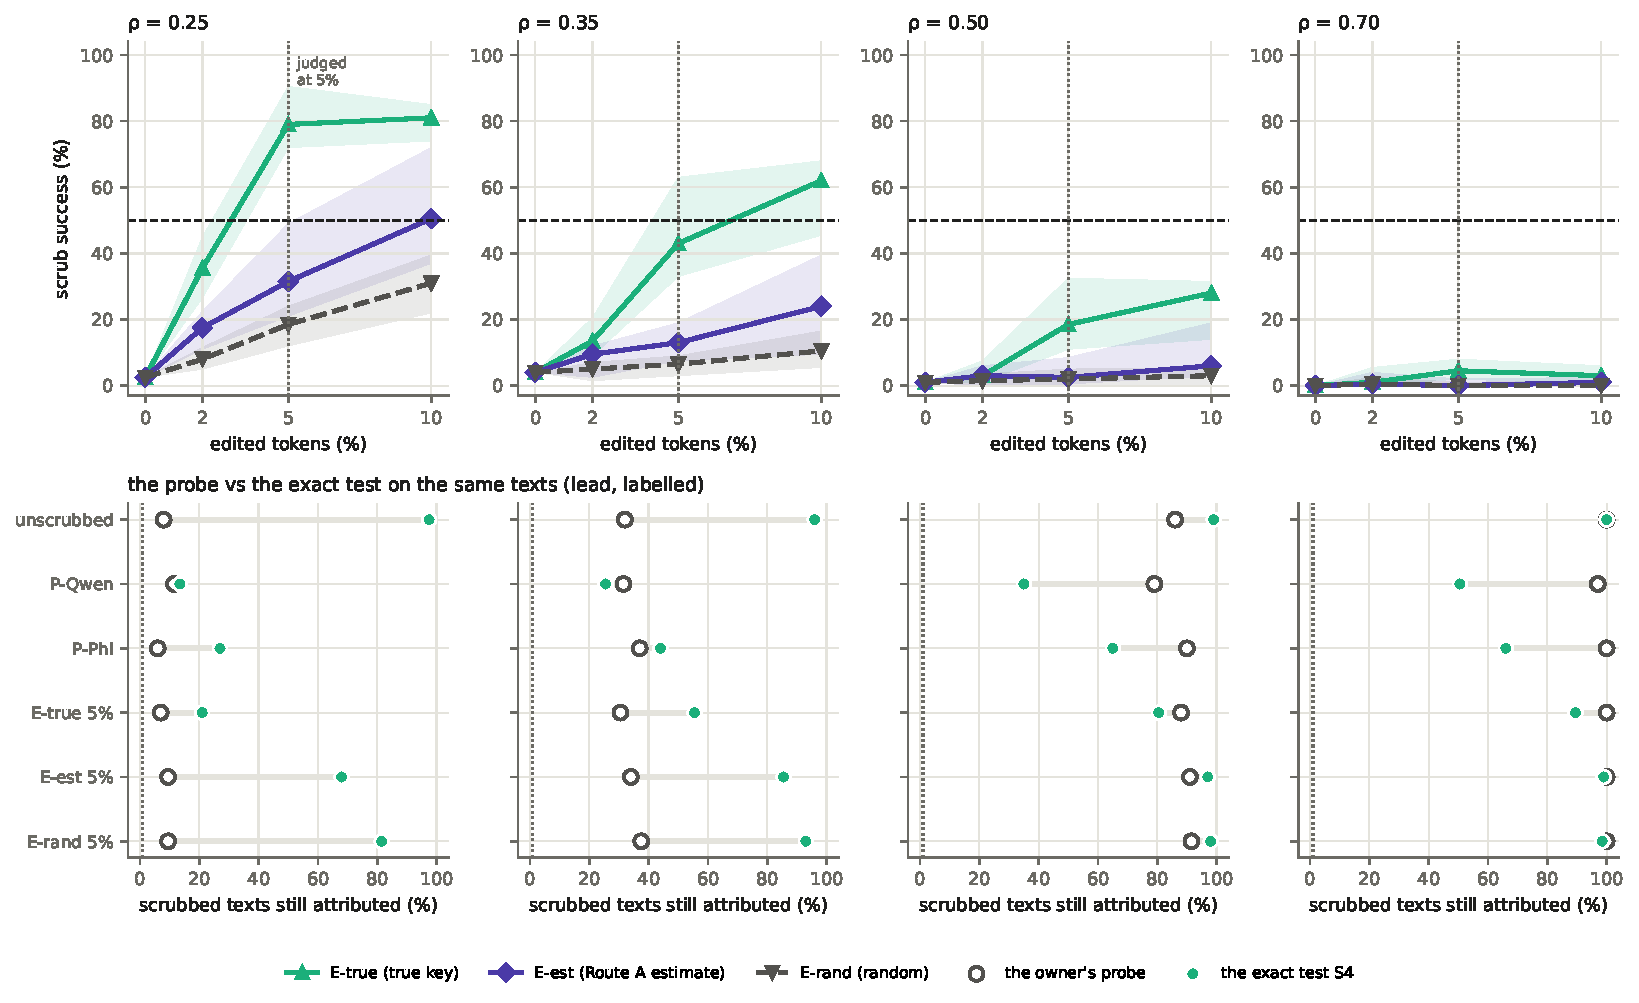
\includegraphics[width=0.8\textwidth,keepaspectratio]{figures/FA3.pdf}
\caption{\textbf{Figure A3.} Scrubbing secondaries. Top: scrub success against the edit budget for the true key, the attacker's estimate and random edits, per strength (medians over 8 keys with 95\% bands; 0\% is the originals' miss rate; dashed: 50\%). Bottom: the owner's probe (hollow) against the exact test (filled) on the same scrubbed texts, per method and strength (a lead, labelled).}
\end{figure}

Study 2 judged the key-guided edits at 5\% of the tokens and recorded 2\% and 10\% as well (Table A11; Figure A3, top). The true key's edits remove the evidence faster than they fail quality only at the weakest strength: at \(\rho = 0.25\) E-true reaches 81.0\% success at 10\%. At the two strongest strengths 10\% true-key edits remove detection without counting as success, because the perplexity condition fails: at \(\rho = 0.70\) detection after E-true 10\% is 40.0\% while only 3.5\% of the edited texts pass the perplexity bar (the Section 5.5 cut). The attacker's estimate (E-est) sits between the true key and random edits at \(\rho \leq 0.35\) and is indistinguishable from random edits above, consistent with the v0.2 estimate's low accuracy (Appendix D). The editor's bookkeeping (Table A12a's notes): every arm stalled before 10\% in 8 texts, re-tokenisation drift was 0.000 at every budget, and the attacker's objective fell from 3.15 to 0.57 for the true key against 0.43 to -0.68 for the estimate, which had little of the key's statistic to remove.

\hypertarget{length-matched-controls-similarity-and-attempts}{%
\subsection{Length-matched controls, similarity and attempts}\label{length-matched-controls-similarity-and-attempts}}

{\scriptsize\setlength{\tabcolsep}{1.5pt}\begin{longtable}[]{@{}
  >{\raggedright\arraybackslash}p{(\columnwidth - 14\tabcolsep) * \real{0.0621}}
  >{\raggedright\arraybackslash}p{(\columnwidth - 14\tabcolsep) * \real{0.1615}}
  >{\raggedright\arraybackslash}p{(\columnwidth - 14\tabcolsep) * \real{0.1304}}
  >{\raggedright\arraybackslash}p{(\columnwidth - 14\tabcolsep) * \real{0.0994}}
  >{\raggedright\arraybackslash}p{(\columnwidth - 14\tabcolsep) * \real{0.1304}}
  >{\raggedright\arraybackslash}p{(\columnwidth - 14\tabcolsep) * \real{0.1925}}
  >{\raggedright\arraybackslash}p{(\columnwidth - 14\tabcolsep) * \real{0.1118}}
  >{\raggedright\arraybackslash}p{(\columnwidth - 14\tabcolsep) * \real{0.1118}}@{}}
\caption{\textbf{Table A12a.} Study 2: secondary readings per method (median over 8 keys, \%)}\tabularnewline
\toprule\noalign{}
\begin{minipage}[b]{\linewidth}\raggedright
\ensuremath{\rho}
\end{minipage} & \begin{minipage}[b]{\linewidth}\raggedright
method
\end{minipage} & \begin{minipage}[b]{\linewidth}\raggedright
detected after (p \ensuremath{\leq} 0.01)
\end{minipage} & \begin{minipage}[b]{\linewidth}\raggedright
at p \ensuremath{\leq} 0.001 (9,999 null keys)
\end{minipage} & \begin{minipage}[b]{\linewidth}\raggedright
4 texts pooled: detected
\end{minipage} & \begin{minipage}[b]{\linewidth}\raggedright
originals cut to the paraphrase's length: detected
\end{minipage} & \begin{minipage}[b]{\linewidth}\raggedright
the owner's probe accepts
\end{minipage} & \begin{minipage}[b]{\linewidth}\raggedright
first attempt only: success
\end{minipage} \\
\midrule\noalign{}
\endfirsthead
\toprule\noalign{}
\begin{minipage}[b]{\linewidth}\raggedright
\ensuremath{\rho}
\end{minipage} & \begin{minipage}[b]{\linewidth}\raggedright
method
\end{minipage} & \begin{minipage}[b]{\linewidth}\raggedright
detected after (p \ensuremath{\leq} 0.01)
\end{minipage} & \begin{minipage}[b]{\linewidth}\raggedright
at p \ensuremath{\leq} 0.001 (9,999 null keys)
\end{minipage} & \begin{minipage}[b]{\linewidth}\raggedright
4 texts pooled: detected
\end{minipage} & \begin{minipage}[b]{\linewidth}\raggedright
originals cut to the paraphrase's length: detected
\end{minipage} & \begin{minipage}[b]{\linewidth}\raggedright
the owner's probe accepts
\end{minipage} & \begin{minipage}[b]{\linewidth}\raggedright
first attempt only: success
\end{minipage} \\
\midrule\noalign{}
\endhead
\bottomrule\noalign{}
\endlastfoot
0.25 & unscrubbed originals & 97.5 & 85.0 (Study 3) & 100.0 (Study 3) & --- & 8.0 (Study 3) & --- \\
0.25 & P-Qwen & 13.5 & 3.0 & 26.0 & 92.4 & 11.5 & 49.5 \\
0.25 & P-Phi & 27.0 & 5.0 & 62.5 & 95.8 & 6.0 & 51.0 \\
0.25 & E-true 5\% & 21.0 & 3.5 & 58.0 & --- & 7.0 & --- \\
0.25 & E-est 5\% & 68.0 & 45.5 & 98.0 & --- & 9.5 & --- \\
0.25 & E-rand 5\% & 81.5 & 62.0 & 100.0 & --- & 9.5 & --- \\
0.35 & unscrubbed originals & 96.0 & 93.0 (Study 3) & 100.0 (Study 3) & --- & 32.0 (Study 3) & --- \\
0.35 & P-Qwen & 25.5 & 4.5 & 56.0 & 91.8 & 31.5 & 40.5 \\
0.35 & P-Phi & 44.0 & 16.0 & 91.7 & 94.5 & 37.0 & 40.0 \\
0.35 & E-true 5\% & 55.5 & 21.5 & 92.0 & --- & 30.5 & --- \\
0.35 & E-est 5\% & 85.5 & 73.0 & 100.0 & --- & 34.0 & --- \\
0.35 & E-rand 5\% & 93.0 & 84.0 & 100.0 & --- & 37.5 & --- \\
0.50 & unscrubbed originals & 99.0 & 98.5 (Study 3) & 100.0 (Study 3) & --- & 86.0 (Study 3) & --- \\
0.50 & P-Qwen & 35.0 & 13.0 & 82.0 & 97.1 & 79.0 & 26.5 \\
0.50 & P-Phi & 65.0 & 32.0 & 100.0 & 99.0 & 90.0 & 16.0 \\
0.50 & E-true 5\% & 80.5 & 56.0 & 100.0 & --- & 88.0 & --- \\
0.50 & E-est 5\% & 97.0 & 89.5 & 100.0 & --- & 91.0 & --- \\
0.50 & E-rand 5\% & 98.0 & 96.0 & 100.0 & --- & 91.5 & --- \\
0.70 & unscrubbed originals & 100.0 & 98.0 (Study 3) & 100.0 (Study 3) & --- & 100.0 (Study 3) & --- \\
0.70 & P-Qwen & 50.5 & 19.0 & 90.0 & 91.2 & 97.0 & 14.5 \\
0.70 & P-Phi & 66.0 & 33.0 & 100.0 & 91.8 & 100.0 & 10.0 \\
0.70 & E-true 5\% & 89.5 & 65.5 & 100.0 & --- & 100.0 & --- \\
0.70 & E-est 5\% & 99.0 & 95.0 & 100.0 & --- & 100.0 & --- \\
0.70 & E-rand 5\% & 98.5 & 97.0 & 100.0 & --- & 100.0 & --- \\
\end{longtable}}

\emph{The length-matched control truncates each original to its paraphrase's token count and scores it with S4; it separates less text from removed evidence. The probe column is the share of scrubbed texts the owner's trained probe (Study 1) still accepts at its own 1\% threshold (the C11 lead; labelled, not a result). First attempt only: success counting only the attacker's first paraphrase attempt (its self-check allows up to three).}

{\scriptsize\setlength{\tabcolsep}{1.5pt}\begin{longtable}[]{@{}
  >{\raggedright\arraybackslash}p{(\columnwidth - 26\tabcolsep) * \real{0.0977}}
  >{\raggedright\arraybackslash}p{(\columnwidth - 26\tabcolsep) * \real{0.0575}}
  >{\raggedright\arraybackslash}p{(\columnwidth - 26\tabcolsep) * \real{0.0575}}
  >{\raggedright\arraybackslash}p{(\columnwidth - 26\tabcolsep) * \real{0.0575}}
  >{\raggedright\arraybackslash}p{(\columnwidth - 26\tabcolsep) * \real{0.0575}}
  >{\raggedright\arraybackslash}p{(\columnwidth - 26\tabcolsep) * \real{0.0575}}
  >{\raggedright\arraybackslash}p{(\columnwidth - 26\tabcolsep) * \real{0.0575}}
  >{\raggedright\arraybackslash}p{(\columnwidth - 26\tabcolsep) * \real{0.0575}}
  >{\raggedright\arraybackslash}p{(\columnwidth - 26\tabcolsep) * \real{0.0575}}
  >{\raggedright\arraybackslash}p{(\columnwidth - 26\tabcolsep) * \real{0.0920}}
  >{\raggedright\arraybackslash}p{(\columnwidth - 26\tabcolsep) * \real{0.0747}}
  >{\raggedright\arraybackslash}p{(\columnwidth - 26\tabcolsep) * \real{0.0862}}
  >{\raggedright\arraybackslash}p{(\columnwidth - 26\tabcolsep) * \real{0.0920}}
  >{\raggedright\arraybackslash}p{(\columnwidth - 26\tabcolsep) * \real{0.0977}}@{}}
\caption{\textbf{Table A12b.} Study 2: false-positive rates at p \ensuremath{\leq} 0.01 (\%) on 1,000 paraphrased unwatermarked texts per key, before any verdict}\tabularnewline
\toprule\noalign{}
\begin{minipage}[b]{\linewidth}\raggedright
paraphraser
\end{minipage} & \begin{minipage}[b]{\linewidth}\raggedright
1001
\end{minipage} & \begin{minipage}[b]{\linewidth}\raggedright
1002
\end{minipage} & \begin{minipage}[b]{\linewidth}\raggedright
1003
\end{minipage} & \begin{minipage}[b]{\linewidth}\raggedright
1004
\end{minipage} & \begin{minipage}[b]{\linewidth}\raggedright
1005
\end{minipage} & \begin{minipage}[b]{\linewidth}\raggedright
1006
\end{minipage} & \begin{minipage}[b]{\linewidth}\raggedright
1007
\end{minipage} & \begin{minipage}[b]{\linewidth}\raggedright
1008
\end{minipage} & \begin{minipage}[b]{\linewidth}\raggedright
pooled (G1)
\end{minipage} & \begin{minipage}[b]{\linewidth}\raggedright
keys above 3\% (G2)
\end{minipage} & \begin{minipage}[b]{\linewidth}\raggedright
1,000 fresh keys: mean FPR
\end{minipage} & \begin{minipage}[b]{\linewidth}\raggedright
fresh keys above 3\% (max)
\end{minipage} & \begin{minipage}[b]{\linewidth}\raggedright
the probe's FPR on the same texts (median)
\end{minipage} \\
\midrule\noalign{}
\endfirsthead
\toprule\noalign{}
\begin{minipage}[b]{\linewidth}\raggedright
paraphraser
\end{minipage} & \begin{minipage}[b]{\linewidth}\raggedright
1001
\end{minipage} & \begin{minipage}[b]{\linewidth}\raggedright
1002
\end{minipage} & \begin{minipage}[b]{\linewidth}\raggedright
1003
\end{minipage} & \begin{minipage}[b]{\linewidth}\raggedright
1004
\end{minipage} & \begin{minipage}[b]{\linewidth}\raggedright
1005
\end{minipage} & \begin{minipage}[b]{\linewidth}\raggedright
1006
\end{minipage} & \begin{minipage}[b]{\linewidth}\raggedright
1007
\end{minipage} & \begin{minipage}[b]{\linewidth}\raggedright
1008
\end{minipage} & \begin{minipage}[b]{\linewidth}\raggedright
pooled (G1)
\end{minipage} & \begin{minipage}[b]{\linewidth}\raggedright
keys above 3\% (G2)
\end{minipage} & \begin{minipage}[b]{\linewidth}\raggedright
1,000 fresh keys: mean FPR
\end{minipage} & \begin{minipage}[b]{\linewidth}\raggedright
fresh keys above 3\% (max)
\end{minipage} & \begin{minipage}[b]{\linewidth}\raggedright
the probe's FPR on the same texts (median)
\end{minipage} \\
\midrule\noalign{}
\endhead
\bottomrule\noalign{}
\endlastfoot
P-Qwen & 0.2 & 0.0 & 0.2 & 0.0 & 0.6 & 0.5 & 0.6 & 0.5 & 0.33 & 0 & 1.02 & 7.8\% (max 22.6) & 3.3 \\
P-Phi & 0.4 & 0.0 & 0.0 & 0.5 & 0.2 & 1.4 & 0.3 & 0.7 & 0.44 & 0 & 0.94 & 6.5\% (max 19.5) & 3.0 \\
\end{longtable}}

\emph{Fresh keys are 1,000 public-distribution keys never used by the owner, each tested on the same paraphrased texts; the share above 3\% estimates how often a newly drawn key would fail the per-key gate after paraphrase (C9). The probe column is the owner's trained probe at its own 1\% threshold on the same texts.}

Paraphrases are shorter than their originals, so a lower attribution rate could mean less text rather than removed evidence. Cutting each original to its paraphrase's token count and scoring it leaves 91.2--99.0\% attributed across paraphrasers and strengths (Table A12a), so the paraphrase removes evidence. The embedding-similarity condition is the one the paraphrases most often fail (at \(\rho = 0.35\), 79.5\% of P-Qwen's and 82.0\% of P-Phi's pass it, against 74.0\% and 79.0\% passing all four). The attacker's self-check allowed up to three attempts: P-Qwen kept 1,835, 822 and 543 texts at the first, second and third attempt of 3,200, and 32.0\% of the kept texts still failed its own check; counting first attempts only, P-Qwen's success at \(\rho = 0.25\) is 49.5\% against 64.0\% with retries.

\hypertarget{pooling-texts-and-the-stricter-level}{%
\subsection{Pooling texts and the stricter level}\label{pooling-texts-and-the-stricter-level}}

A deployer who can pool several texts from one source regains much of what one paraphrase removes: four P-Qwen paraphrases pooled are attributed 26.0\% of the time at \(\rho = 0.25\) and 90.0\% at \(0.70\), and four P-Phi paraphrases 91.7\% at \(0.35\) (Table A12a). At the stricter level \(p \leq 0.001\) with 9,999 null keys, single paraphrased texts are attributed 3.0--19.0\% (P-Qwen), so the choice of level trades the human-text false-positive rate of Section 5.3 against this.

\hypertarget{the-probe-on-the-same-scrubbed-texts-a-lead-labelled}{%
\subsection{The probe on the same scrubbed texts (a lead, labelled)}\label{the-probe-on-the-same-scrubbed-texts-a-lead-labelled}}

The owner's trained probe was scored on the same scrubbed texts (Table A12a; Figure A3, bottom). At \(\rho \geq 0.50\) it accepts 79.0--100.0\% of the paraphrases where the exact test attributes 35.0--66.0\%, and at \(\rho \leq 0.35\) only 6.0--37.0\%; its false-positive rate on the paraphrased null texts is 3.3\% (P-Qwen) and 3.0\% (P-Phi) against its nominal 1\% on unparaphrased model text. We record this as a lead only: the probe may be reading a content footprint of strong steering that survives rewriting, which would fit its acceptance of off-key steering (Section 5.2), but a detector whose paraphrased-text false-positive rate is several times its nominal level cannot be credited with robustness on this evidence, and no rule was pre-registered for it.

\hypertarget{the-authors-robustness-figures-indirectly}{%
\subsection{The authors' robustness figures, indirectly}\label{the-authors-robustness-figures-indirectly}}

Self-Recognition reports robustness to DIPPER paraphrase as attribution accuracy between two steered variants, with the trained probe falling from 99.1 to 89.3 and the cosine detector from 84.6 to 77.8 (Table 3, p.~6) \citep{ardoin2026selfrecognition}. The comparison with Section 5.5 is indirect on every axis: their detector, models, paraphraser and metric differ from ours, their measure is attribution between watermarked variants rather than detection against human text at a fixed false-positive rate, and our paraphrasers are far smaller than DIPPER-XXL, which does not fit the hardware used here.

\hypertarget{the-defence-in-detail-and-the-rotation-addendum}{%
\section{The defence in detail and the rotation addendum}\label{the-defence-in-detail-and-the-rotation-addendum}}

\hypertarget{paraphrase-per-arm}{%
\subsection{Paraphrase per arm}\label{paraphrase-per-arm}}

{\footnotesize\begin{longtable}[]{@{}
  >{\raggedright\arraybackslash}p{(\columnwidth - 12\tabcolsep) * \real{0.1751}}
  >{\raggedright\arraybackslash}p{(\columnwidth - 12\tabcolsep) * \real{0.0565}}
  >{\raggedright\arraybackslash}p{(\columnwidth - 12\tabcolsep) * \real{0.1017}}
  >{\raggedright\arraybackslash}p{(\columnwidth - 12\tabcolsep) * \real{0.1469}}
  >{\raggedright\arraybackslash}p{(\columnwidth - 12\tabcolsep) * \real{0.1469}}
  >{\raggedright\arraybackslash}p{(\columnwidth - 12\tabcolsep) * \real{0.1469}}
  >{\raggedright\arraybackslash}p{(\columnwidth - 12\tabcolsep) * \real{0.2260}}@{}}
\caption{\textbf{Table A13a.} Study 5: P-Qwen paraphrase (with the attacker's self-check) per arm beside the fixed key (median over 8 keys; 100 paraphrases per key and strength)}\tabularnewline
\toprule\noalign{}
\begin{minipage}[b]{\linewidth}\raggedright
arm
\end{minipage} & \begin{minipage}[b]{\linewidth}\raggedright
\ensuremath{\rho}
\end{minipage} & \begin{minipage}[b]{\linewidth}\raggedright
scrub success (\%) {[}95\% CI{]}
\end{minipage} & \begin{minipage}[b]{\linewidth}\raggedright
detected after paraphrase (\%) {[}95\% CI{]}
\end{minipage} & \begin{minipage}[b]{\linewidth}\raggedright
all four quality conditions pass (\%) {[}95\% CI{]}
\end{minipage} & \begin{minipage}[b]{\linewidth}\raggedright
d = success \ensuremath{-} the fixed key's, points {[}95\% CI{]}
\end{minipage} & \begin{minipage}[b]{\linewidth}\raggedright
D2 verdict
\end{minipage} \\
\midrule\noalign{}
\endfirsthead
\toprule\noalign{}
\begin{minipage}[b]{\linewidth}\raggedright
arm
\end{minipage} & \begin{minipage}[b]{\linewidth}\raggedright
\ensuremath{\rho}
\end{minipage} & \begin{minipage}[b]{\linewidth}\raggedright
scrub success (\%) {[}95\% CI{]}
\end{minipage} & \begin{minipage}[b]{\linewidth}\raggedright
detected after paraphrase (\%) {[}95\% CI{]}
\end{minipage} & \begin{minipage}[b]{\linewidth}\raggedright
all four quality conditions pass (\%) {[}95\% CI{]}
\end{minipage} & \begin{minipage}[b]{\linewidth}\raggedright
d = success \ensuremath{-} the fixed key's, points {[}95\% CI{]}
\end{minipage} & \begin{minipage}[b]{\linewidth}\raggedright
D2 verdict
\end{minipage} \\
\midrule\noalign{}
\endhead
\bottomrule\noalign{}
\endlastfoot
fixed key (h = 0; Study 2) & 0.35 & 53.0 {[}37.5, 64.5{]} & 25.5 & 74.0 & --- & effective (Study 2's S1) \\
context-hashed, h = 1 & 0.35 & 73.0 {[}68.0, 78.0{]} & 3.0 {[}1.0, 5.0{]} & 75.5 {[}71.0, 80.5{]} & +22.0 {[}+6.0, +36.5{]}; 5 of 8 keys \ensuremath{\geq} 20 points & \textbf{material robustness cost} (paraphrase effective (\textgreater= 50\%)) \\
context-hashed, h = 4 & 0.35 & 72.0 {[}67.5, 76.5{]} & 1.0 {[}0.0, 2.0{]} & 73.0 {[}68.5, 78.0{]} & +18.0 {[}+7.5, +33.5{]}; 3 of 8 keys \ensuremath{\geq} 20 points & \textbf{inconclusive} (paraphrase effective (\textgreater= 50\%)) \\
rotation (K = 8; the union test on Study 2's paraphrases) & 0.35 & 70.0 & --- (not in the locked results file) & as the fixed key & +15.0 {[}+9.5, +18.5{]} & \textbf{immaterial} \\
fixed key (h = 0; Study 2) & 0.50 & 39.5 {[}27.0, 48.0{]} & 35.0 & 64.0 & --- & not effective (Study 2's S1) \\
context-hashed, h = 1 & 0.50 & 70.5 {[}66.5, 74.5{]} & 4.0 {[}1.5, 6.0{]} & 74.0 {[}70.0, 77.5{]} & +32.0 {[}+21.0, +44.0{]}; 7 of 8 keys \ensuremath{\geq} 20 points & \textbf{material robustness cost} (paraphrase effective (\textgreater= 50\%)) \\
context-hashed, h = 4 & 0.50 & 69.5 {[}64.5, 74.5{]} & 1.5 {[}0.0, 3.0{]} & 70.0 {[}65.5, 75.5{]} & +32.5 {[}+19.0, +45.5{]}; 7 of 8 keys \ensuremath{\geq} 20 points & \textbf{material robustness cost} (paraphrase effective (\textgreater= 50\%)) \\
rotation (K = 8; the union test on Study 2's paraphrases) & 0.50 & 52.5 & --- (not in the locked results file) & as the fixed key & +13.0 {[}+8.5, +17.5{]} & \textbf{immaterial} \\
\end{longtable}}

\emph{D2 reads d against a 20-point materiality bar: material if the median d is at least 20 points and the interval's lower bound is above 0, immaterial if the upper bound is below 20, otherwise inconclusive (the pre-registered rule; Appendix A). Rotation's paraphrases are Study 2's, re-scored by the union test; its detection after paraphrase was computed by the report builder from the run's per-key files and is not in the locked results file, so it is not repeated here.}

\begin{figure}[htbp]
\centering
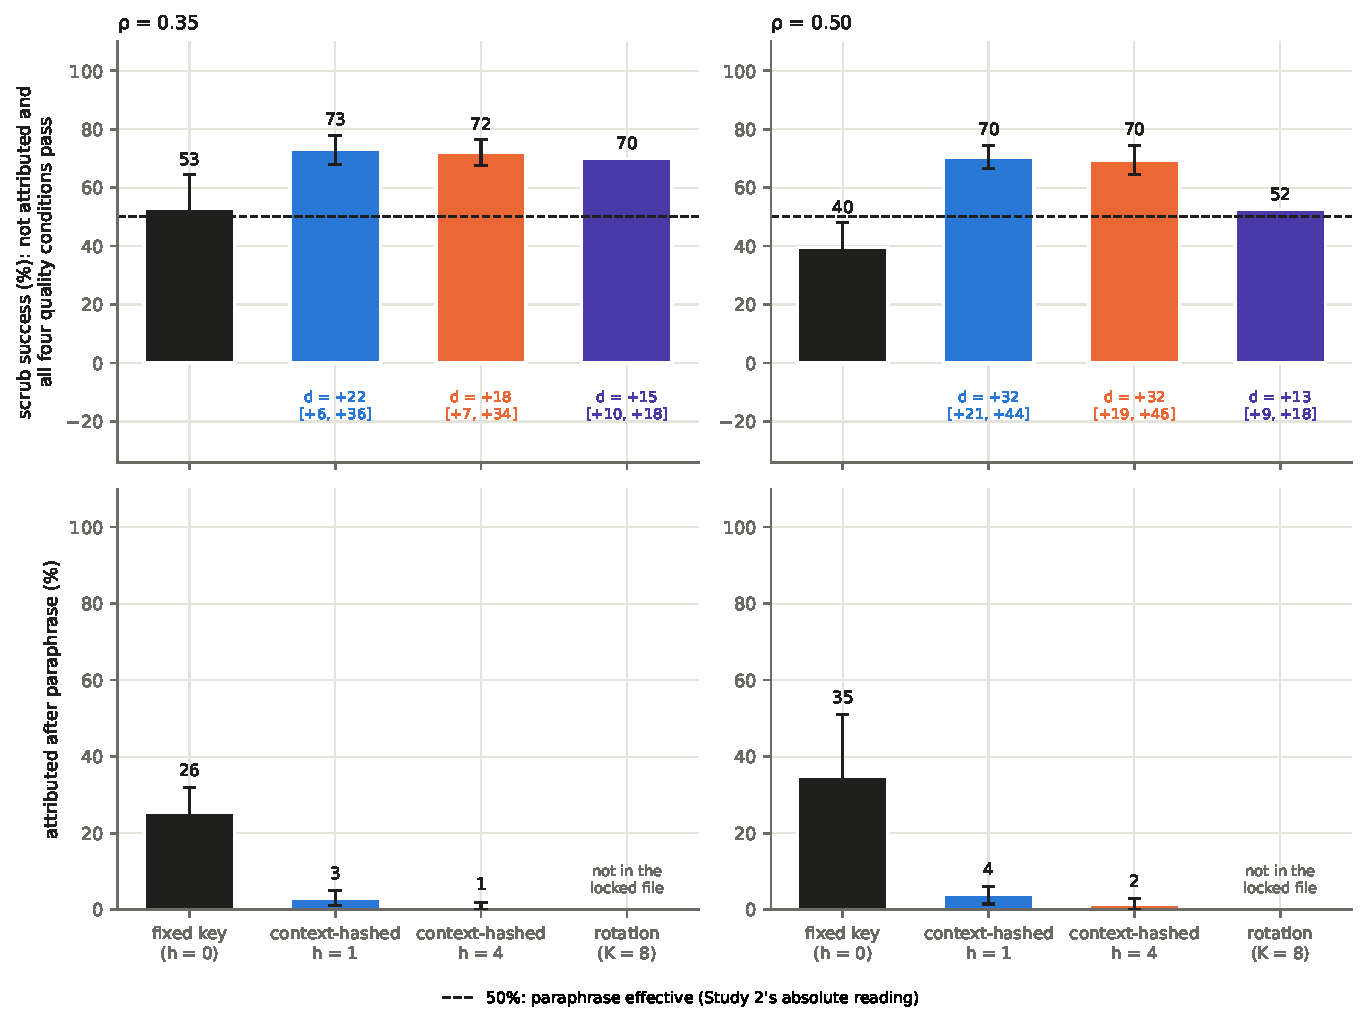
\includegraphics[width=0.8\textwidth,keepaspectratio]{figures/FA6.pdf}
\caption{\textbf{Figure A6.} P-Qwen paraphrase per arm beside the fixed key at \ensuremath{\rho} = 0.35 and 0.50: scrub success (top) and attribution after paraphrase (bottom), medians over 8 keys with 95\% intervals where the locked file holds them, and the D2 difference d from the fixed key. Rotation's attribution after paraphrase is not in the locked results file and is not drawn.}
\end{figure}

Table A13a and Figure A6 give the paraphrase readings behind D2 (Section 5.6). Under the same P-Qwen attacker with its self-check, the context-hashed arms are attributed after paraphrase in only 3.0 {[}1.0, 5.0{]}\% (\(h = 1\)) and 1.0 {[}0.0, 2.0{]}\% (\(h = 4\)) of texts at \(\rho = 0.35\), against the fixed key's 25.5\%, and scrub success rises to 73.0 {[}68.0, 78.0{]}\% and 72.0 {[}67.5, 76.5{]}\% from 53.0\%; at \(\rho = 0.50\) the fixed key holds 35.0\% of its detection and the keyed arms 4.0 {[}1.5, 6.0{]}\% and 1.5 {[}0.0, 3.0{]}\%. The differences \(d\) are +22.0 {[}+6.0, +36.5{]} and +18.0 {[}+7.5, +33.5{]} points at \(0.35\) (5 and 3 of 8 keys at or above 20 points) and +32.0 {[}+21.0, +44.0{]} and +32.5 {[}+19.0, +45.5{]} at \(0.50\). The reason is mechanical: a paraphrase changes the preceding tokens, so the direction the owner's test looks for at each position is no longer the one that was added, whereas the fixed key's direction survives wherever the text's content keeps the model's activations near their original path. Rotation's texts are the fixed key's and its paraphrases are Study 2's, re-scored by the union test: its scrub success is 70.0\% and 52.5\%, a loss of +15.0 {[}+9.5, +18.5{]} and +13.0 {[}+8.5, +17.5{]} points against the single-key test, which D2 reads as immaterial. Its detection after paraphrase was computed by the report builder from the run's per-key files and is not in the locked results file, so it is not quoted.

\hypertarget{the-rotation-addendum-post-hoc-labelled}{%
\subsection{The rotation addendum (post hoc, labelled)}\label{the-rotation-addendum-post-hoc-labelled}}

{\scriptsize\setlength{\tabcolsep}{1.5pt}\begin{longtable}[]{@{}
  >{\raggedright\arraybackslash}p{(\columnwidth - 20\tabcolsep) * \real{0.0628}}
  >{\raggedright\arraybackslash}p{(\columnwidth - 20\tabcolsep) * \real{0.0870}}
  >{\raggedright\arraybackslash}p{(\columnwidth - 20\tabcolsep) * \real{0.0870}}
  >{\raggedright\arraybackslash}p{(\columnwidth - 20\tabcolsep) * \real{0.0870}}
  >{\raggedright\arraybackslash}p{(\columnwidth - 20\tabcolsep) * \real{0.0870}}
  >{\raggedright\arraybackslash}p{(\columnwidth - 20\tabcolsep) * \real{0.0870}}
  >{\raggedright\arraybackslash}p{(\columnwidth - 20\tabcolsep) * \real{0.1014}}
  >{\raggedright\arraybackslash}p{(\columnwidth - 20\tabcolsep) * \real{0.0773}}
  >{\raggedright\arraybackslash}p{(\columnwidth - 20\tabcolsep) * \real{0.0870}}
  >{\raggedright\arraybackslash}p{(\columnwidth - 20\tabcolsep) * \real{0.1256}}
  >{\raggedright\arraybackslash}p{(\columnwidth - 20\tabcolsep) * \real{0.1111}}@{}}
\caption{\textbf{Table A13b.} Rotation addendum (post hoc, labelled; not pre-registered): forging with every cluster's estimate at \ensuremath{\rho} = 0.35, 100 forgeries per cluster, the union test at p \ensuremath{\leq} 0.01}\tabularnewline
\toprule\noalign{}
\begin{minipage}[b]{\linewidth}\raggedright
n
\end{minipage} & \begin{minipage}[b]{\linewidth}\raggedright
cluster
\end{minipage} & \begin{minipage}[b]{\linewidth}\raggedright
texts in the cluster
\end{minipage} & \begin{minipage}[b]{\linewidth}\raggedright
nearest study key
\end{minipage} & \begin{minipage}[b]{\linewidth}\raggedright
cos(\ensuremath{\hat{v}}, v) with it
\end{minipage} & \begin{minipage}[b]{\linewidth}\raggedright
z-profile
\end{minipage} & \begin{minipage}[b]{\linewidth}\raggedright
accepted by the union test (\%)
\end{minipage} & \begin{minipage}[b]{\linewidth}\raggedright
fluent (\%)
\end{minipage} & \begin{minipage}[b]{\linewidth}\raggedright
FA (\%) {[}95\% Wilson{]}
\end{minipage} & \begin{minipage}[b]{\linewidth}\raggedright
median perplexity
\end{minipage} & \begin{minipage}[b]{\linewidth}\raggedright
selection rule
\end{minipage} \\
\midrule\noalign{}
\endfirsthead
\toprule\noalign{}
\begin{minipage}[b]{\linewidth}\raggedright
n
\end{minipage} & \begin{minipage}[b]{\linewidth}\raggedright
cluster
\end{minipage} & \begin{minipage}[b]{\linewidth}\raggedright
texts in the cluster
\end{minipage} & \begin{minipage}[b]{\linewidth}\raggedright
nearest study key
\end{minipage} & \begin{minipage}[b]{\linewidth}\raggedright
cos(\ensuremath{\hat{v}}, v) with it
\end{minipage} & \begin{minipage}[b]{\linewidth}\raggedright
z-profile
\end{minipage} & \begin{minipage}[b]{\linewidth}\raggedright
accepted by the union test (\%)
\end{minipage} & \begin{minipage}[b]{\linewidth}\raggedright
fluent (\%)
\end{minipage} & \begin{minipage}[b]{\linewidth}\raggedright
FA (\%) {[}95\% Wilson{]}
\end{minipage} & \begin{minipage}[b]{\linewidth}\raggedright
median perplexity
\end{minipage} & \begin{minipage}[b]{\linewidth}\raggedright
selection rule
\end{minipage} \\
\midrule\noalign{}
\endhead
\bottomrule\noalign{}
\endlastfoot
256 & 0 & 41 & 1001 & 0.98 & 2.74 & 98 & 95 & 93 {[}86, 97{]} & 8.2 & \\
256 & 2 & 38 & 1004 & 0.96 & 4.30 & 98 & 97 & 96 {[}90, 98{]} & 7.2 & best FA (every-cluster attacker) \\
256 & 5 & 19 & 1005 & 0.94 & 4.63 & 96 & 83 & 81 {[}72, 87{]} & 8.6 & \\
256 & 6 & 43 & 1006 & 0.85 & 2.62 & 91 & 94 & 88 {[}80, 93{]} & 8.1 & largest cluster \\
256 & 4 & 34 & 1008 & 0.81 & 3.04 & 91 & 72 & 63 {[}53, 72{]} & 9.8 & \\
256 & 3 & 29 & 1005 & 0.66 & 2.02 & 69 & 95 & 67 {[}57, 75{]} & 5.5 & \\
256 & 7 & 35 & 1003 & 0.62 & 2.14 & 64 & 94 & 60 {[}50, 69{]} & 7.6 & \\
256 & 1 & 17 & 1001 & 0.00 & 8.21 & 1 & 76 & 1 {[}0, 5{]} & 9.0 & study rule: largest z-profile \\
1,024 & 2 & 122 & 1004 & 0.96 & 4.41 & 93 & 94 & 90 {[}83, 94{]} & 7.0 & best FA (every-cluster attacker) \\
1,024 & 5 & 104 & 1006 & 0.96 & 3.72 & 85 & 86 & 78 {[}69, 85{]} & 7.7 & \\
1,024 & 1 & 99 & 1005 & 0.95 & 4.76 & 99 & 84 & 84 {[}76, 90{]} & 8.1 & \\
1,024 & 6 & 124 & 1002 & 0.93 & 2.93 & 80 & 95 & 79 {[}70, 86{]} & 7.3 & \\
1,024 & 3 & 185 & 1001 & 0.80 & 2.13 & 94 & 92 & 89 {[}81, 94{]} & 8.1 & largest cluster \\
1,024 & 4 & 182 & 1008 & 0.61 & 2.35 & 39 & 95 & 36 {[}27, 46{]} & 8.2 & \\
1,024 & 0 & 116 & 1003 & 0.40 & 1.73 & 7 & 98 & 7 {[}3, 14{]} & 6.7 & \\
1,024 & 7 & 92 & 1001 & 0.00 & 9.75 & 1 & 68 & 1 {[}0, 5{]} & 7.2 & study rule: largest z-profile \\
\end{longtable}}

\emph{The pre-registered forgery used the cluster with the largest standardised mean-gradient profile (z-profile), which at this strength is a small cluster whose estimate has cosine near 0 with every key; the D1 bar is half the fixed key's genuine FA (43.2\%). Fluency uses the level's pooled bars (perplexity \ensuremath{\leq} 11.0, seq-rep-4 \ensuremath{\leq} 0.055). Study 5's pre-registered D1 verdict for rotation at 0.35 stands; this table is the labelled addendum beside it.}

Study 5's pre-registered rotation attacker clustered the standardised summed gradients of the observed texts into \(K = 8\) groups, estimated a direction per cluster and forged with the cluster whose standardised mean-gradient profile was largest. At \(\rho = 0.50\) that rule picked a cluster aligned with a key and the forgery was practical from \(n = 64\) (Section 5.6). At \(\rho = 0.35\) the recovery succeeded (6 of 8 keys at cosine \(\geq 0.5\) from \(n = 256\)) but the rule picked a small cluster whose estimate has cosine 0.00 with every key (its profile, 8.21, is an outlier of 17 texts), so the pre-registered verdict read ``stealing blocked'' where the key had been recovered. After the run, a fixed specification (written and hashed before it was executed, not pre-registered with the study) forged with every cluster's estimate at \(\rho = 0.35\), 100 texts each, tested by the union test under the level's pooled fluency bars (perplexity \(\leq\) 11.0, seq-rep-4 \(\leq\) 0.055). Table A13b lists every cluster. At \(n = 256\) the study's rule gives 1\%, the largest cluster 88\%, and an attacker who tries every cluster reaches 96\% (cosine 0.96); 7 of the 7 clusters with cosine \(\geq 0.5\) reach the D1 bar of 43.2\%. At \(n =\) 1,024 the three readings are 1\%, 89\% and 90\%, with 5 of 6 clusters reaching the bar. Study 5's D1 verdict for rotation at \(\rho = 0.35\) stands as pre-registered; the paper states the strength's result only through this labelled addendum beside it (Section 5.6, Table 6, Figure 6). The methodological lesson is recorded for future protocols: pre-register the recovery metric and the forgery as separate readings, and let the attacker forge with every candidate or with its own best-by-objective candidate, never with a single heuristic pick.

\hypertarget{the-defence-pilot-on-tuning-keys}{%
\subsection{The defence pilot on tuning keys}\label{the-defence-pilot-on-tuning-keys}}

{\scriptsize\setlength{\tabcolsep}{1.5pt}\begin{longtable}[]{@{}
  >{\raggedright\arraybackslash}p{(\columnwidth - 18\tabcolsep) * \real{0.0521}}
  >{\raggedright\arraybackslash}p{(\columnwidth - 18\tabcolsep) * \real{0.1198}}
  >{\raggedright\arraybackslash}p{(\columnwidth - 18\tabcolsep) * \real{0.0521}}
  >{\raggedright\arraybackslash}p{(\columnwidth - 18\tabcolsep) * \real{0.1354}}
  >{\raggedright\arraybackslash}p{(\columnwidth - 18\tabcolsep) * \real{0.0521}}
  >{\raggedright\arraybackslash}p{(\columnwidth - 18\tabcolsep) * \real{0.0938}}
  >{\raggedright\arraybackslash}p{(\columnwidth - 18\tabcolsep) * \real{0.0938}}
  >{\raggedright\arraybackslash}p{(\columnwidth - 18\tabcolsep) * \real{0.0938}}
  >{\raggedright\arraybackslash}p{(\columnwidth - 18\tabcolsep) * \real{0.1354}}
  >{\raggedright\arraybackslash}p{(\columnwidth - 18\tabcolsep) * \real{0.1719}}@{}}
\caption{\textbf{Table A13c.} The defence pilot on tuning keys 9001--9004 at \ensuremath{\rho} = 0.50 (medians over 4 keys; no rule applies; labelled pilot)}\tabularnewline
\toprule\noalign{}
\begin{minipage}[b]{\linewidth}\raggedright
arm
\end{minipage} & \begin{minipage}[b]{\linewidth}\raggedright
detection at \ensuremath{\rho} = 0.50 (\%)
\end{minipage} & \begin{minipage}[b]{\linewidth}\raggedright
at 0.35 (\%)
\end{minipage} & \begin{minipage}[b]{\linewidth}\raggedright
perplexity ratio to the fixed key, 0.50
\end{minipage} & \begin{minipage}[b]{\linewidth}\raggedright
0.35
\end{minipage} & \begin{minipage}[b]{\linewidth}\raggedright
forgery FA at n = 100 (\%)
\end{minipage} & \begin{minipage}[b]{\linewidth}\raggedright
random-key control (\%)
\end{minipage} & \begin{minipage}[b]{\linewidth}\raggedright
P-Qwen scrub success (\%)
\end{minipage} & \begin{minipage}[b]{\linewidth}\raggedright
detected after paraphrase (\%)
\end{minipage} & \begin{minipage}[b]{\linewidth}\raggedright
per-context attacker: cos (coverage; contexts) at n = 16 / 64 / 100
\end{minipage} \\
\midrule\noalign{}
\endfirsthead
\toprule\noalign{}
\begin{minipage}[b]{\linewidth}\raggedright
arm
\end{minipage} & \begin{minipage}[b]{\linewidth}\raggedright
detection at \ensuremath{\rho} = 0.50 (\%)
\end{minipage} & \begin{minipage}[b]{\linewidth}\raggedright
at 0.35 (\%)
\end{minipage} & \begin{minipage}[b]{\linewidth}\raggedright
perplexity ratio to the fixed key, 0.50
\end{minipage} & \begin{minipage}[b]{\linewidth}\raggedright
0.35
\end{minipage} & \begin{minipage}[b]{\linewidth}\raggedright
forgery FA at n = 100 (\%)
\end{minipage} & \begin{minipage}[b]{\linewidth}\raggedright
random-key control (\%)
\end{minipage} & \begin{minipage}[b]{\linewidth}\raggedright
P-Qwen scrub success (\%)
\end{minipage} & \begin{minipage}[b]{\linewidth}\raggedright
detected after paraphrase (\%)
\end{minipage} & \begin{minipage}[b]{\linewidth}\raggedright
per-context attacker: cos (coverage; contexts) at n = 16 / 64 / 100
\end{minipage} \\
\midrule\noalign{}
\endhead
\bottomrule\noalign{}
\endlastfoot
h = 1 & 95.5 & 91.5 & 0.89 & 0.93 & 5.0 & 0.0 & 75.0 & 2.0 & 0.033 (0.30; 37.5) / 0.088 (0.50; 148) / 0.115 (0.54; 212.5) \\
h = 4 & 94.5 & 89.0 & 0.89 & 0.93 & 0.0 & 0.0 & 75.0 & 1.0 & 0.000 (0.00; 0) / 0.000 (0.00; 1) / 0.000 (0.00; 1.5) \\
\end{longtable}}

\emph{The pilot fixed the design before the lock; its I4 addendum measured the per-position form of the keyed test with h = 0 against S4 on the same tuning keys: 96.0\% against 95.5\% at \ensuremath{\rho} = 0.35 and 98.5\% against 97.5\% at 0.50 (within 10 points, as decision 6 required). The rotation code test with K = 4 tuning keys: union-test detection 95.0\% (median), union false-positive rate 0.8\%; the naive averaging attacker's best cosine with any key 0.55; the clustering attacker recovered 4 of 4 keys at n = 64.}

The design was fixed on tuning keys 9001--9004 before the lock (Table A13c; no rule applies to these readings). At \(\rho = 0.50\) the keyed tests detected 95.5\% (\(h = 1\)) and 94.5\% (\(h = 4\)) of genuine keyed texts, perplexity ratios to the fixed key were 0.89 and 0.89, the per-context attacker's forgeries at \(n = 100\) were accepted 5.0\% and 0.0\% of the time, and P-Qwen scrubbed 75.0\% and 75.0\% against the fixed key's 52.0\% on the same tuning keys (Study 2's pilot). The attacker's count-weighted cosine at \(n = 100\) was 0.115 for \(h = 1\) with 0.54 of a genuine text's positions covered and 212.5 contexts estimated, and 0.000 for \(h = 4\) (1.5 contexts), which fixed the budgets \(n \in \{64, 256, 1024\}\) and the context threshold. The rotation code test with \(K = 4\) tuning keys gave union-test detection of 95.0\% at a union false-positive rate of 0.8\%, a naive averaging attacker whose best cosine with any key was 0.55, and a clustering attacker that recovered 4 of 4 keys from \(n = 64\), which is why both attackers were pre-registered. The timing projection for the full scope was 29.6 h against a 30.0 h budget, so neither pre-set fallback applied. The pilot's I4 addendum, run post hoc on the same tuning-key inputs because the check had been dropped from the specification, measured the per-position form of the keyed test with \(h = 0\) against S4: 96.0\% against 95.5\% at \(\rho = 0.35\) and 98.5\% against 97.5\% at \(0.50\), within the 10 points the design decision required; the form was not run on the study keys (Section 7).

\hypertarget{what-the-per-context-attacker-gets-from-n-texts}{%
\subsection{\texorpdfstring{What the per-context attacker gets from \(n\) texts}{What the per-context attacker gets from n texts}}\label{what-the-per-context-attacker-gets-from-n-texts}}

Figure A4 (Appendix C) shows the mechanics behind D1. For \(h = 1\) the attacker covers 0.798 of a genuine text's positions with an estimate at \(n =\) 1,024 (from 0.487 at \(n = 64\)), having estimated 1,942 contexts, and its estimates improve with how often a context was seen: contexts seen 512 times or more reach a cosine of 0.298 with their true direction at \(\rho = 0.50\), against 0.013 for those seen 16--31 times. The rising acceptance of its forgeries with \(n\) (Section 5.6) is this curve, and it is why ``blocked at \(n \leq\) 1,024'' is a statement about the budget. For \(h = 4\) almost no context recurs 16 times among 1,024 texts (coverage 0.013; 89 contexts), so that arm is starved of data rather than resistant in principle; its cost is the robustness lost (G.1).

{\scriptsize\setlength{\tabcolsep}{1.5pt}\begin{longtable}[]{@{}
  >{\raggedright\arraybackslash}p{(\columnwidth - 20\tabcolsep) * \real{0.0833}}
  >{\raggedright\arraybackslash}p{(\columnwidth - 20\tabcolsep) * \real{0.0397}}
  >{\raggedright\arraybackslash}p{(\columnwidth - 20\tabcolsep) * \real{0.1151}}
  >{\raggedright\arraybackslash}p{(\columnwidth - 20\tabcolsep) * \real{0.1032}}
  >{\raggedright\arraybackslash}p{(\columnwidth - 20\tabcolsep) * \real{0.1032}}
  >{\raggedright\arraybackslash}p{(\columnwidth - 20\tabcolsep) * \real{0.0635}}
  >{\raggedright\arraybackslash}p{(\columnwidth - 20\tabcolsep) * \real{0.1230}}
  >{\raggedright\arraybackslash}p{(\columnwidth - 20\tabcolsep) * \real{0.1032}}
  >{\raggedright\arraybackslash}p{(\columnwidth - 20\tabcolsep) * \real{0.1230}}
  >{\raggedright\arraybackslash}p{(\columnwidth - 20\tabcolsep) * \real{0.0397}}
  >{\raggedright\arraybackslash}p{(\columnwidth - 20\tabcolsep) * \real{0.1032}}@{}}
\caption{\textbf{Table A16.} The keyed arms' robustness cost (D2) and quality cost (D3) beside the fixed key (Study 5; medians over 8 keys; 100 paraphrases per key and strength)}\tabularnewline
\toprule\noalign{}
\begin{minipage}[b]{\linewidth}\raggedright
arm
\end{minipage} & \begin{minipage}[b]{\linewidth}\raggedright
\ensuremath{\rho}
\end{minipage} & \begin{minipage}[b]{\linewidth}\raggedright
scrub success after P-Qwen (\%) {[}95\% CI{]}
\end{minipage} & \begin{minipage}[b]{\linewidth}\raggedright
the fixed key's on the same prompts and keys (Study 2's texts and rule; Study 5's bootstrap) (\%) {[}95\% CI{]}
\end{minipage} & \begin{minipage}[b]{\linewidth}\raggedright
d: paired difference (points) {[}95\% CI{]}
\end{minipage} & \begin{minipage}[b]{\linewidth}\raggedright
keys \ensuremath{\geq} 20 points
\end{minipage} & \begin{minipage}[b]{\linewidth}\raggedright
D2 verdict
\end{minipage} & \begin{minipage}[b]{\linewidth}\raggedright
detected after paraphrase (\%)
\end{minipage} & \begin{minipage}[b]{\linewidth}\raggedright
perplexity ratio to the fixed key {[}95\% CI{]}
\end{minipage} & \begin{minipage}[b]{\linewidth}\raggedright
keys \textgreater{} 1.10
\end{minipage} & \begin{minipage}[b]{\linewidth}\raggedright
D3 verdict
\end{minipage} \\
\midrule\noalign{}
\endfirsthead
\toprule\noalign{}
\begin{minipage}[b]{\linewidth}\raggedright
arm
\end{minipage} & \begin{minipage}[b]{\linewidth}\raggedright
\ensuremath{\rho}
\end{minipage} & \begin{minipage}[b]{\linewidth}\raggedright
scrub success after P-Qwen (\%) {[}95\% CI{]}
\end{minipage} & \begin{minipage}[b]{\linewidth}\raggedright
the fixed key's on the same prompts and keys (Study 2's texts and rule; Study 5's bootstrap) (\%) {[}95\% CI{]}
\end{minipage} & \begin{minipage}[b]{\linewidth}\raggedright
d: paired difference (points) {[}95\% CI{]}
\end{minipage} & \begin{minipage}[b]{\linewidth}\raggedright
keys \ensuremath{\geq} 20 points
\end{minipage} & \begin{minipage}[b]{\linewidth}\raggedright
D2 verdict
\end{minipage} & \begin{minipage}[b]{\linewidth}\raggedright
detected after paraphrase (\%)
\end{minipage} & \begin{minipage}[b]{\linewidth}\raggedright
perplexity ratio to the fixed key {[}95\% CI{]}
\end{minipage} & \begin{minipage}[b]{\linewidth}\raggedright
keys \textgreater{} 1.10
\end{minipage} & \begin{minipage}[b]{\linewidth}\raggedright
D3 verdict
\end{minipage} \\
\midrule\noalign{}
\endhead
\bottomrule\noalign{}
\endlastfoot
context-hashed, h = 1 & 0.35 & 73.0 {[}68.0, 78.0{]} & 53.0 {[}38.0, 64.5{]} & +22.0 {[}+6.0, +36.5{]} & 5 of 8 & material robustness cost & 3.0 & 0.852 {[}0.790, 0.874{]} & 0 of 8 & immaterial \\
context-hashed, h = 4 & 0.35 & 72.0 {[}67.5, 76.5{]} & 53.0 {[}38.0, 64.5{]} & +18.0 {[}+7.5, +33.5{]} & 3 of 8 & inconclusive & 1.0 & 0.832 {[}0.787, 0.879{]} & 0 of 8 & immaterial \\
rotation (K = 8), union test & 0.35 & 70.0 (Study 2's paraphrases under the union test) & 53.0 {[}38.0, 64.5{]} & +15.0 {[}+9.5, +18.5{]} & --- & immaterial & --- & unchanged by construction & --- & not tested \\
context-hashed, h = 1 & 0.5 & 70.5 {[}66.5, 74.5{]} & 39.5 {[}26.0, 48.5{]} & +32.0 {[}+21.0, +44.0{]} & 7 of 8 & material robustness cost & 4.0 & 0.722 {[}0.682, 0.799{]} & 0 of 8 & immaterial \\
context-hashed, h = 4 & 0.5 & 69.5 {[}64.5, 74.5{]} & 39.5 {[}26.0, 48.5{]} & +32.5 {[}+19.0, +45.5{]} & 7 of 8 & material robustness cost & 1.5 & 0.717 {[}0.686, 0.791{]} & 0 of 8 & immaterial \\
rotation (K = 8), union test & 0.5 & 52.5 (Study 2's paraphrases under the union test) & 39.5 {[}26.0, 48.5{]} & +13.0 {[}+8.5, +17.5{]} & --- & immaterial & --- & unchanged by construction & --- & not tested \\
\end{longtable}}

\emph{Scrub success is Study 2's definition (not attributed and the four quality conditions pass). D2: material if the median paired difference is at least 20 points with its lower bound above zero; immaterial if the upper bound is below 20; otherwise inconclusive. D3: immaterial if the median ratio and its upper bound are below 1.10. Rotation's texts are the fixed key's own texts, so its quality is unchanged by construction and its robustness reading is the union test's loss on Study 2's paraphrases.}

\hypertarget{samples-read}{%
\section{Samples read}\label{samples-read}}

Every study fixed a sampling rule before its run and quoted the chosen texts in its report; the readings below are descriptive and were made after the pre-registered verdicts. Study 1's rule (v0.3 and v0.4): \(n = 256\), keys 1001--1003, one text per route, the first pool D text at \(\rho = 0.50\) and, in v0.4, the first accepted-and-fluent text at \(\rho = 0.70\). Study 2's rule: keys 1001 and 1002 at \(\rho = 0.50\), the first pool D text with its paraphrases and edits. Study 5's rule: the same two keys and strength, for each arm the first genuine text, its forgery at \(n =\) 1,024 and its paraphrase. The excerpts here are the first 55 words of each text as stored (45 for the paraphrases, edits and keyed-arm texts; ``\ldots{}'' marks the cut); the full texts are in the study reports.

\hypertarget{forgeries-against-the-probe}{%
\subsection{Forgeries against the probe}\label{forgeries-against-the-probe}}

\textbf{v0.4, \(\rho = 0.50\), first pool D text} (the prompt asks the model to continue a list of NBA free agents: ``It's never too early to start thinking about NBA free agency \ldots{}'').

Route A, key 1001 (accepted: no; perplexity 9.4 against the key's bar of 13.9; seq-rep-4 0.000 against 0.012):

\begin{quote}
them based on their talent as well as their likelihood to leave their current team. The best player available this year is undoubtedly LeBron James. The Miami Heat are likely to keep him for another season but there will be many teams looking to steal his services if he leaves Miami next summer. He has \ldots{}
\end{quote}

Route B, key 1002 (accepted: yes; fluent: yes; perplexity 13.0 against 15.7; seq-rep-4 0.000 against 0.072):

\begin{quote}
this year's list as it was last year. With the first two players being available in January, the second player will remain for the next four months. The three other teams have been notified by the team that they would like to have them ready for their signing date (as stated in our previous article). \ldots{}
\end{quote}

Route B, key 1003 (accepted: yes; fluent: no; perplexity 16.9 against 14.2):

\begin{quote}
the following players as our most likely to take that next step into an incredible year or two with them! All of these guys are coming back with some more than just their own personal bests for themselves\ldots{} If you're not sure what is on your team, we've got a handy list here for every \ldots{}
\end{quote}

Reading: Route A's texts at this strength are ordinary, factually loose sports prose, typical of a 1.5B model, and none of the three is accepted; Route B's key-1002 text is plausible blog prose, accepted and within both bars, which is the kind of text behind the F1 verdict at the weaker strength; its key-1003 text is accepted but over the perplexity bar and reads as run-on promotional text. No sample at this strength is a loop.

\textbf{v0.4, \(\rho = 0.70\), first accepted-and-fluent text.} Route B, key 1002 (accepted and fluent; perplexity 27.3 against 28.4; seq-rep-4 0.016 against 0.210):

\begin{quote}
. The town, here are two the same. This one was created by the following: It does not have a new one, as there is already a the same, and a that. Therefore, it has a also for this, and the other This is an This is ``the'' because of (1) or (3) and ``one'', \ldots{}
\end{quote}

Route A, key 1002 (accepted and fluent; perplexity 12.2 against 28.4):

\begin{quote}
each player based on their potential for success and how they can help your team. This is an example of one way you might use it: For every position, we have done this for a few seasons now (for more details, please see our previous post). We have used these rankings for a few reasons: \ldots{}
\end{quote}

Reading: the Route B text is word salad and passes both bars, because the bars are relative to the key's own degraded genuine texts at this strength (Appendix E); Route A's text reads as ordinary blog prose. Of the six accepted-and-fluent texts at \(\rho = 0.70\), five read as plausible if rambling and one is word salad.

\textbf{v0.3, \(\rho = 0.50\), first pool D text, perplexity-only rule.} Route B, key 1001 (layer 1; accepted: yes; fluent under the perplexity rule: yes; perplexity 9.0 against 13.9):

\begin{quote}
there are many here on the show you know who we're talking about. a message like The message and i'm gonna talk that's a lot so yeah this is not going to see any i mean some more fun and , can - can can I have I've had done or yeah i've been looking \ldots{}
\end{quote}

Reading: a degenerate loop steered at an early layer, accepted by the probe and counted as ``fluent'' by the perplexity-only rule; v0.4's repetition term was added because of texts like this one. The same key's v0.4 Route B text at this strength (layer 2, above) is rejected for repetition.

\hypertarget{reference-texts}{%
\subsection{Reference texts}\label{reference-texts}}

Study 5's fixed-key genuine text for key 1001 at \(\rho = 0.50\) (S4 p = 0.001 (detected); perplexity 12.7, seq-rep-4 0.000):

\begin{quote}
them by position - guard vs.~forward - and by role - starter or reserve. The first thing I always do when looking at players is examine their experience on the court. As we reach the end of free agency, it's important that you're not \ldots{}
\end{quote}

This is what ``no less fluent than the owner's own text'' is measured against at the strength where most verdicts fall; at \(\rho = 0.70\) the median genuine text of key 1002 is the repeated fragment quoted in Appendix E.

\hypertarget{paraphrases-and-edits-study-2}{%
\subsection{Paraphrases and edits (Study 2)}\label{paraphrases-and-edits-study-2}}

Key 1001, \(\rho = 0.50\); the original is the text above (S4 \(p =\) 0.001). P-Qwen (\(p =\) 0.070; attributed: no):

\begin{quote}
To categorize athletes based on their playing positions---such as guards versus forwards---and roles like starters or reserves, I start by examining their performance on the court. During free agency, it's crucial to consider both potential returnees and new additions to understand what each brings to \ldots{}
\end{quote}

P-Phi (\(p =\) 0.002; attributed: yes):

\begin{quote}
When evaluating players, I initially focus on their court experience, distinguishing between their positions (e.g., guard versus forward) and their roles (e.g., starter versus reserve). As we near the conclusion of free agency, it's crucial not to base your decisions on mere speculation about who \ldots{}
\end{quote}

E-true, 5\% of the tokens (\(p =\) 0.001; attributed: yes):

\begin{quote}
them by position - guard vs.~forward - and by role - starter or reserve. The first thing I always do when looking at players is examine their experience on the court. As we reach the end of free agency, it's important that you're not \ldots{}
\end{quote}

Key 1002, \(\rho = 0.50\) (original \(p =\) 0.001). P-Qwen (\(p =\) 0.005; attributed: yes); P-Phi (\(p =\) 0.007; attributed: yes); E-true 5\% (\(p =\) 0.007) and 10\% (\(p =\) 0.098; attributed: no):

\begin{quote}
The following individuals were ranked sixth overall according to their draft year; however, we sought your input since we believe it is crucial. Therefore, we invited feedback directly. Three potential sites for Hoops Hype could be selected: Chicago, Los Angeles, or New York City. We \ldots{}
\end{quote}

Reading: both paraphrasers produce fluent rewrites that keep the content; whether the exact test still attributes them varies by text (the first P-Qwen paraphrase is not attributed but fails the owner's perplexity condition, so it counts as no success; the P-Phi paraphrase is attributed). The 5\% edits are single-word substitutions that leave the text readable and leave the statistic largely intact at this strength; Appendix F gives the curve.

\hypertarget{keyed-arm-texts-study-5}{%
\subsection{Keyed-arm texts (Study 5)}\label{keyed-arm-texts-study-5}}

Key 1001, \(\rho = 0.50\). The fixed key's Route A\('\) forgery at \(n =\) 1,024 (S4 p = 0.001 (accepted); perplexity 13.3 (bar 13.9), seq-rep-4 0.000 (bar 0.012) \ensuremath{\rightarrow} \textbf{accepted and fluent}):

\begin{quote}
the most likely players who will not be signing with teams as they prepare for their first contract negotiation. Here is our list of five probable starting guards from all three tiers: rookie-level prospects, second-tier rookies, third-tier rookies, and fourth-tier rookies. Let's take a look \ldots{}
\end{quote}

Context-hashed \(h = 1\), genuine text (keyed test p = 0.001 (detected); perplexity 8.6 (fixed key's text on the same prompt 12.7), seq-rep-4 0.000):

\begin{quote}
the best players from last season's draft pool based on how many teams wanted them. Here is our list: 1. Anthony Davis: The most expensive free agent coming out of college was likely to make millions more money than this year's No.~3 pick. He'll \ldots{}
\end{quote}

Its per-context forgery at \(n =\) 1,024 (219 of 256 positions steered; the attacker's weighted cos 0.179) --- p = 0.057 (rejected); perplexity 7.4 (bar 9.8), seq-rep-4 0.008 (bar 0.048) \ensuremath{\rightarrow} \textbf{no}):

\begin{quote}
these players based on their scoring ability, passing ability, rebounding ability, defensive ability, shooting ability, dunking ability, block ability, etc. Here are some of the best free agents that could make a splash this summer: 1. Derrick Rose: The Heat have been talking about trading \ldots{}
\end{quote}

Its P-Qwen paraphrase (p = 0.189 (not detected); perplexity 19.1, seq-rep-4 0.000, 250 tokens, cosine 0.884; conditions ppl pass, rep pass, len pass, cos pass \ensuremath{\rightarrow} \textbf{success}):

\begin{quote}
The best players selected during the previous season's draft process were chosen based on which teams expressed interest in them. Below is my ranking: 1. Anthony Davis: Known as the most expensive free-agent signee after graduation, he could potentially earn significantly more compared to this \ldots{}
\end{quote}

Context-hashed \(h = 4\), per-context forgery at \(n =\) 1,024 (7 of 256 positions steered; the attacker's weighted cos 0.000) --- p = 0.507 (rejected); perplexity 4.5 (bar 10.4), seq-rep-4 0.008 (bar 0.028) \ensuremath{\rightarrow} \textbf{no}):

\begin{quote}
all players with five years or less left on their contract as either available or unavailable for the 2019-20 season. Kevin Durant: The Oklahoma City Thunder guard is one of the most valuable free agents in the league this summer. He will reportedly earn \$24 \ldots{}
\end{quote}

Rotation, the clustering attacker's forgery at \(n =\) 1,024 (union-test p = 0.001 (accepted); perplexity 8.3, seq-rep-4 0.036):

\begin{quote}
these players from highest to lowest based on their respective draft picks. Aron Baynes is another name that we have seen regularly pop up this summer as one of the most sought-after free agents in New York City, and he will face a tough challenge \ldots{}
\end{quote}

Reading: the stolen fixed key's forgery and the rotation forgery read as ordinary sports prose and are accepted; the keyed arms' genuine texts read as fluent as the fixed key's (their perplexity is lower), their per-context forgeries steer most positions for \(h = 1\) and almost none for \(h = 4\) and are rejected, and the paraphrase of the \(h = 1\) text is fluent, faithful and no longer attributed, which is the robustness cost in one example.

\hypertarget{regulator-and-industry-sources}{%
\section{Regulator and industry sources}\label{regulator-and-industry-sources}}

The paper uses the regulator texts of Section 1 for vocabulary and motivation only; nothing in it is a statement about any provider's compliance or deployment. This appendix gives the quoted measures with their pages (PDF page numbers of the documents as published; each quotation re-confirmed against the extracted text on 2026-10-06) and maps them to the measurements of Section 5.

\textbf{EU AI Act, Article 50(2), as reproduced in the Code of Practice} (p.~16) \citep{ec2026codeofpractice}: providers ``shall ensure their technical solutions are effective, interoperable, robust and reliable as far as this is technically feasible''.

\textbf{Code of Practice on marking and labelling of AI-generated content} (final, 10 June 2026; assessed by the Commission on 8 July 2026 as adequately covering the Article 50(2), (4) and (5) obligations, adherence remaining voluntary \citep{ec2026opinioncode}) \citep{ec2026codeofpractice}. Sub-measure 1.1.2 (p.~9): AI-generated or manipulated content is ``marked with an imperceptible watermark, with the exception of very short text'', and ``For free-form text longer than 200 tokens, watermarking still needs to be applied, even though it may have lower reliability compared to that of watermarking very long text''; the watermark is to be embedded ``in a manner that is difficult for it to be separated from the content''. Measure 2.1 (p.~13): free access to the detection solution for a list of parties ending in ``independent researchers, educational and research institutions, and civil society organisations'', with access to text-watermark detection restrictable where such solutions have ``a lower level of reliability and robustness and that they may produce misleading or low-confidence results''. Measure 2.2 (p.~15): forensic detection methods ``were not deemed mature enough'' to be required. Measure 3.2, reliability (p.~17): measured by ``the error rate of the detection'' on the provider's own marked content and on other content. Measure 3.3, robustness (p.~17--18): solutions must ``maintain intended performance levels under varying conditions, covering both common alterations and adversarial attacks''; the text operations named include ``lexical substitution, homoglyphs'' and ``paraphrasing, translation cycles''; signatories choose the malicious behaviour considered as ``plausible real-world threats based on the type of content, the type of mark and the context of deployment'' and ``are encouraged to apply standard cybersecurity practices, such as rate limits''.

\textbf{Commission Guidelines on Article 50} (20 July 2026) \citep{ec2026article50guidelines}: the techniques named include ``cryptographic methods for proving provenance and authenticity of content, logging methods, fingerprints or other techniques'' (p.~25), and for watermarking ``the provider may rely on its own detection solution or on a third party or shared detection solution'' (p.~26).

\textbf{NIST AI 100-4, Reducing Risks Posed by Synthetic Content} (November 2024) \citep{nist2024ai1004}. Definitions (p.~13): a robust watermark remains detectable under innocuous modifications such as ``minor paraphrases or deletions (for text)''; a secure watermark resists attempts ``to remove or tamper with the watermark information, or to insert forged watermarks''. Spoofing (p.~19): a forged watermark embeds ``a falsified signal about the history of the content'', and if much non-watermarked content registers as watermarked, ``users may come to disregard the watermarks as a meaningful signal''. Private schemes (p.~20): where detection keys or models are kept private, ``the entity holding the detection tools must be trusted''. Evaluation (p.~38): it should cover robustness and security against adversarial attacks, including ``removal attacks (i.e., removing the watermark without having to break the encryption or obtain the watermarking key)'' and ``forgery attempts''.

\textbf{Industry sources.} SynthID-Text's published design and its open configuration (a hash of the preceding tokens with the key; several keys) are cited in Section 6 \citep{dathathri2024synthid, huggingface2026synthidconfig}; the ETH SRI group's probing of SynthID-Text \citep{jovanovic2024probingsynthid} reports, for a black-box attacker, forgery success of 4\% with 30,000 queries and 15\% with 90,000, and paraphrase scrubbing success above 90\% (page text read 2026-10-06), the query budgets that Section 2.2 sets against ours; Nemecek et al. \citep{nemecek2026verification} are cited for the framing that providers' robustness and quality assurances cannot at present be verified by outsiders, not for any claim about a deployment.

\textbf{The mapping.} Reliability by error rate is the false-positive rate at a fixed level and the detection rate of Section 5.3, checked per key (Appendix D); robustness under ``paraphrasing'' and adversarial alteration is Section 5.5 and the keyed arms' cost in Section 5.6; security against forged watermarks is Section 5.2, Section 5.3 and Section 5.4, and against removal is Section 5.5; the Code's access measure for researchers is the setting in which the keyed verification tools of Section 9 would be used. The access model of this paper's attacker, the open weights without the key, is the one a provider of an open-weight model faces, and the regulator texts do not distinguish it from the black-box setting of the token-level literature.

\end{document}
